\documentclass[
	12pt,					% tamanho da fonte
	openright,				% capítulos começam em pág ímpar (insere página vazia caso preciso)
	oneside,				% para impressão em recto e verso (twoside). Oposto a (oneside)
	a4paper,				% tamanho do papel.
	chapter=TITLE,			% títulos de capítulos convertidos em letras maiúsculas
	section=TITLE,			% títulos de seções convertidos em letras maiúsculas
	sumario=abnt-6027-2012,
	english,				% idioma adicional para hifenização
	brazil,					% o último idioma é o principal do documento
	fleqn,					% equações alinhadas a esquerda (UDESC/CCT)+
	]{abntex2}

% ----------------------------------------------------------
% Pacotes básicos
% ----------------------------------------------------------
% \usepackage{Pacotes/abntex2}
\usepackage{amsmath, amssymb, amsfonts, amsthm, mathtools}
\usepackage{mathptmx} 							% Usa a fonte Times New Roman	 (UDESC/CCT)
\usepackage[T1]{fontenc}						% Seleção de códigos de fonte.
\usepackage[utf8]{inputenc}						% Codificação do documento (conversão automática dos acentos)
\usepackage{lastpage}							% Usado pela Ficha catalográfica
\usepackage{indentfirst}						% Indenta o primeiro parágrafo de cada seção.
\usepackage[dvipsnames,table]{xcolor}			% Controle das cores
\usepackage{graphicx}							% Inclusão de gráficos
\usepackage{microtype} 							% para melhorias de justificação
\usepackage[brazilian,hyperpageref]{backref}	% Paginas com as citações na bibl
\usepackage[alf,abnt-emphasize=bf,abnt-full-initials=yes]{abntex2cite}					% Citações padrão ABNT
\usepackage{adjustbox}							% Pacote de ajuste de boxes
\usepackage{subcaption}							% Inclusão de Subfiguras e sublegendas
\usepackage{enumitem}							% Personalização de listas
\usepackage[section]{placeins}					% Manter as figuras delimitadas na respectiva seção com a opção [section]
\usepackage{multirow}							% Multi colunas nas tabelas
\usepackage{array,tabularx} 					% Pacotes de tabelas
\usepackage{booktabs}							% Pacote de tabela profissional
\usepackage{rotating}							% Rotacionar figuras e tabelas
\usepackage{xfrac}								% Fazer frações n/d em linha
\usepackage{bm}									% Negrito em modo matemático
\usepackage{xstring}							% Manipulação de strings
\usepackage{chngcntr}							% Pacte usado para deixar numeração de equações sequencial (UDESC/CCT)
\usepackage{xspace}								% Espaçamento após comandos
\usepackage{bussproofs}							% Provas em estilo de árvore
\usepackage{hyperref}							% Suporte para hiperlinks
\usepackage{listings, lstCoq}					% Highlighting de código Coq
\usepackage{tikz}								% Imagens e Diagramas
\usepackage{ulem}								% Texto strikethrough
\usepackage{calrsfs}

\definecolor{darkgreen}{rgb}{0,0.6,0}
\definecolor{darkorange}{rgb}{0.8,0.4,0.2}
\definecolor{darkred}{rgb}{0.8,0,0}

\usetikzlibrary{arrows.meta,positioning,matrix}

\counterwithout{equation}{chapter}
% fonte: https://latex.org/forum/viewtopic.php?t=15392

% Comando para deixar numeração das equações contínua (1), (2), (3)... ao invés de organizar por capítulos (1.1)(1.2)... (2.1)(2.2)
%\renewcommand{\theequation}{\arabic{equation}}

%\numberwithin{equation}{section}


% Cabeçalho somente com numeração de página 10pt
\makepagestyle{PagNumReduzida}
\makeevenhead{PagNumReduzida}{\ABNTEXfontereduzida\thepage}{}{}
\makeoddhead{PagNumReduzida}{}{}{\ABNTEXfontereduzida\thepage}
%fonte: https://github.com/abntex/abntex2/wiki/HowToCustomizarCabecalhoRodape
%fonte: Manual memoir seção 7.3 pg. 111 pdf http://linorg.usp.br/CTAN/macros/latex/contrib/memoir/memman.pdf

% Personalização das opções das listas
\setlist[itemize]{leftmargin=\parindent}

% Citação online --- MODIFICAR ---
\newcommand{\citeshort}[1]{\citeauthoronline{#1} (\citeyear{#1})}

\newcommand{\me}{Elaborado pelo autor.}

% Configuração do pgfplots
% \pgfplotsset{compat=newest} %compat=1.14
% \pgfplotsset{plot coordinates/math parser=false}
% \newlength\figureheight
% \newlength\figurewidth

% Libraries do TiKz
% \usetikzlibrary{quotes,angles,arrows}
% \usetikzlibrary{through,calc,math}
% \usetikzlibrary{graphs,backgrounds,fit}
% \usetikzlibrary{shapes,positioning,patterns,shadows}
% \usetikzlibrary{decorations.pathreplacing}
% \usetikzlibrary{shapes.geometric}
% \usetikzlibrary{arrows.meta}
% \usetikzlibrary{external}

%\tikzexternalize[]
%\tikzexternalenable
%\tikzexternalize
%\tikzexternaldisable
%\tikzset{external/force remake}
%\tikzexternalize[shell escape=-enable-write18]

% Personalização das legendas
\usepackage[format = plain, %hang
			justification = centering,
			labelsep = endash,
			singlelinecheck = false,
			skip = 6pt,
			listformat = simple]{caption}

% Personalizações de tipo de colunas de tabelas
\newcolumntype{L}[1]{>{\raggedright\let\newline\\\arraybackslash\hspace{0pt}}m{#1}}
\newcolumntype{C}[1]{>{\centering\let\newline\\\arraybackslash\hspace{0pt}}m{#1}}
\newcolumntype{R}[1]{>{\raggedleft\let\newline\\\arraybackslash\hspace{0pt}}m{#1}}

% Personalizações de cores da UDESC
\definecolor{CapaAmareloUDESC}{RGB}{243,186,83}		% Especialização
\definecolor{CapaVerdeUDESC}{RGB}{0,112,52}			% Mestrado
\definecolor{CapaVermelhoUDESC}{RGB}{171,35,21}		% Doutorado
\definecolor{CapaAzulUDESC}{RGB}{38,54,118} 		% Pós-Doutorado

% CONFIGURAÇÕES DE PACOTES
% Configurações do pacote backref
% Usado sem a opção hyperpageref de backref
\renewcommand{\backrefpagesname}{Citado na(s) página(s):~}
% Texto padrão antes do número das páginas
\renewcommand{\backref}{}
% Define os textos da citação
\renewcommand*{\backrefalt}[4]{
	\ifcase #1 %
	Nenhuma citação no texto.%
	\or
	Citado na página #2.%
	\else
	Citado #1 vezes nas páginas #2.%
	\fi}%

% alterando o aspecto da cor azul
%\definecolor{blue}{RGB}{41,5,195}

% informações do PDF
\makeatletter
\hypersetup{
	%pagebackref=true,
	pdftitle={\@title},
	pdfauthor={\@author},
	pdfsubject={\imprimirpreambulo},
	pdfcreator={LaTeX with abnTeX2},
	pdfkeywords={abnt}{latex}{abntex}{abntex2}{trabalho academico},
	colorlinks=true,       		% false: boxed links; true: colored links
	linkcolor=blue,          	% color of internal links
	citecolor=blue,        	% color of links to bibliography
	filecolor=blue,      		% color of file links
	urlcolor=blue,			% color of external links
	bookmarksdepth=4
}
\makeatother


% \makeatletter
% \newcommand{\includetikz}[1]{%
% 	\tikzsetnextfilename{#1}%
% 	\input{#1.tex}%
% }
% \makeatother

% ---
% Possibilita criação de Quadros e Lista de quadros.
% Ver https://github.com/abntex/abntex2/issues/176
%
\newcommand{\quadroname}{Quadro}
\newcommand{\listofquadrosname}{Lista de quadros}

\newfloat[chapter]{quadro}{loq}{\quadroname}
\newlistof{listofquadros}{loq}{\listofquadrosname}
\newlistentry{quadro}{loq}{0}

% configurações para atender às regras da ABNT
\setfloatadjustment{quadro}{\centering}
\counterwithout{quadro}{chapter}
\renewcommand{\cftquadroname}{\quadroname\space}
\renewcommand*{\cftquadroaftersnum}{\hfill--\hfill}

\setfloatlocations{quadro}{hbtp} % Ver https://github.com/abntex/abntex2/issues/176
% ---


% Espaçamento depois do título
\setlength{\afterchapskip}{0.7\baselineskip}
% O tamanho do parágrafo é dado por:
\setlength{\parindent}{1.25cm}
% Controle do espaçamento entre um parágrafo e outro:
\setlength{\parskip}{0.0cm}  % tente também \onelineskip
%\SingleSpacing % Espaçamento simples
\OnehalfSpacing % Espaçamento 1,5 (UDESC/CCT)
%\DoubleSpacing	% Espaçamento duplo

% ---
% Margens - NBR 14724/2011 - 5.1 Formato
% ---
\setlrmarginsandblock{3cm}{2cm}{*}
\setulmarginsandblock{3cm}{2cm}{*}
\checkandfixthelayout[fixed]
% ---


% To use externalize consider
%https://tex.stackexchange.com/questions/182783/tikzexternalize-not-compatible-with-miktex-2-9-abntex2-package
%Lauro Cesar digged into the problem until he came with a solution for me to test. And it Works!
%
%According to this link:
%
%The package calc changed the commands \setcounter and friends to be fragile.
% So you have to make them robust. The example below uses etoolbox with \robustify:
%
\usepackage{etoolbox}
\robustify\setcounter
\robustify\addtocounter
\robustify\setlength
\robustify\addtolength


%% How to silence memoir class warning against the use of caption package?
%% https://tex.stackexchange.com/questions/391993/how-to-silence-memoir-class-warning-against-the-use-of-caption-package
%\usepackage{silence}
%\WarningFilter*{memoir}{You are using the caption package with the memoir class}
%\WarningFilter*{Class memoir Warning}{You are using the caption package with the memoir class}

% --------------------------------------------------------
% INICIO DAS CUSTOMIZACOES PARA A UDESC
% --------------------------------------------------------

% --------------------------------------------------------
% Fontes padroes de part, chapter, section, subsection e subsubsection
% --------------------------------------------------------
% --- Chapter ---
\renewcommand{\ABNTEXchapterfont}{\fontseries{b}} %\bfseries
\renewcommand{\ABNTEXchapterfontsize}{\normalsize}
% --- Part ---
\renewcommand{\ABNTEXpartfont}{\ABNTEXchapterfont}
\renewcommand{\ABNTEXpartfontsize}{\LARGE}
% --- Section ---
\renewcommand{\ABNTEXsectionfont}{\normalfont}
\renewcommand{\ABNTEXsectionfontsize}{\normalsize}
% --- SubSection ---
\renewcommand{\ABNTEXsubsectionfont}{\fontseries{b}} %\bfseries
\renewcommand{\ABNTEXsubsectionfontsize}{\normalsize}
% --- SubSubSection ---
\renewcommand{\ABNTEXsubsubsectionfont}{\itshape}
\renewcommand{\ABNTEXsubsubsectionfontsize}{\normalsize}

\renewcommand{\ABNTEXsubsubsubsectionfont}{\normalfont}
\renewcommand{\ABNTEXsubsubsubsectionfontsize}{\normalsize}
% ---

% --------------------------------------------------------
% Fontes das entradas do sumario
% --------------------------------------------------------

\renewcommand{\cftpartfont}{\ABNTEXpartfont\selectfont}
\renewcommand{\cftpartpagefont}{\normalsize\selectfont}

\renewcommand{\cftchapterfont}{\ABNTEXchapterfont\selectfont}
\renewcommand{\cftchapterpagefont}{\normalsize\selectfont}

\renewcommand{\cftsectionfont}{\ABNTEXsectionfont\selectfont}
\renewcommand{\cftsectionpagefont}{\normalsize\selectfont}

\renewcommand{\cftsubsectionfont}{\ABNTEXsubsectionfont\selectfont}
\renewcommand{\cftsubsectionpagefont}{\normalsize\selectfont}

\renewcommand{\cftsubsubsectionfont}{\normalfont\itshape\selectfont}
\renewcommand{\cftsubsubsectionpagefont}{\normalsize\selectfont}

\renewcommand{\cftparagraphfont}{\normalfont\selectfont}
\renewcommand{\cftparagraphpagefont}{\normalsize\selectfont}

% --------------------------------------------------------
% Usando os pacotes hyperref, uppercase...
% Para deixar a section do toc uppercase precisa de:
% --------------------------------------------------------
\usepackage{textcase}

\makeatletter

\let\oldcontentsline\contentsline
\def\contentsline#1#2{%
	\expandafter\ifx\csname l@#1\endcsname\l@section
	\expandafter\@firstoftwo
	\else
	\expandafter\@secondoftwo
	\fi
	{%
		\oldcontentsline{#1}{\MakeTextUppercase{#2}}%
	}{%
		\oldcontentsline{#1}{#2}%
	}%
}
\makeatother

% --------------------------------------------------------
% Renomenando as entradas de APÊNDICES E ANEXOS
% --------------------------------------------------------

\renewcommand{\apendicesname}{AP\^ENDICES}
\renewcommand{\anexosname}{ANEXOS}


% Manipulação de Strings
%\RequirePackage{xstring}

% Comando para inverter sobrenome e nome
\newcommand{\invertname}[1]{%
	\StrBehind{#1}{{}}, \StrBefore{#1}{{}}%
}%


% --------------------------------------------------------
% Alterando os estilos de Caption e Fonte
% --------------------------------------------------------
\makeatletter
% Define o comando \fonte que respeita as configurações de caption do memoir ou do caption
\renewcommand{\fonte}[2][\fontename]{%
	\M@gettitle{#2}%
	\memlegendinfo{#2}%
	\par
	\begingroup
	\@parboxrestore
	\if@minipage
	\@setminipage
	\fi
	\ABNTEXfontereduzida
	\configureseparator
	\captiondelim{\ABNTEXcaptionfontedelim}
	\@makecaption{#1}{\ignorespaces #2}\par
	\endgroup}


\captionstyle[\raggedright]{\raggedright}

\makeatother

\setlength{\cftbeforechapterskip}{0pt plus 0pt}
\renewcommand*{\insertchapterspace}{}

\newlength{\mylen}	% New length to use with spacing
\setlength{\mylen}{1pt}

\setlength{\cftbeforechapterskip}{\mylen}
\setlength{\cftbeforesectionskip}{\mylen}
\setlength{\cftbeforesubsectionskip}{\mylen}
\setlength{\cftbeforesubsubsectionskip}{\mylen}
\setlength{\cftbeforesubsubsubsectionskip}{\mylen}


% ---
% Ajuste das listas de abreviaturas e siglas ; e símbolos [Personalizada para UDESC com espaçamento 1,5]
% ---

% ---
% Redefinição da Lista de abreviaturas e siglas [Personalizada para UDESC com espaçamento 1,5]
\renewenvironment{siglas}{%
	\pretextualchapter{\listadesiglasname}
	\begin{symbols}
		\setlength{\itemsep}{0pt}	% Ajuste para Espaçamento 1,5 (UDESC/CCT)
	}{%
	\end{symbols}
	\cleardoublepage
}
% ---

% ---
% Redefinição da Lista de símbolos [Personalizada para UDESC com espaçamento 1,5]
\renewenvironment{simbolos}{%
	\pretextualchapter{\listadesimbolosname}
	\begin{symbols}
		\setlength{\itemsep}{0pt}	% Ajuste para Espaçamento 1,5 (UDESC/CCT)
	}{%
	\end{symbols}
	\cleardoublepage
}
% ---

% ---
% FIM DAS CUSTOMIZAÇÕES PARA A  Universidade do Estado de Santa Catarina - UDESC/CCT
% ---	% Inclui pacotes básicos

\graphicspath{{Texto/Figuras/}}
\renewcommand{\orientadorname}{Orientadora:}

% O pacote bm torna a fonte do mathcal feia, a linha abaixo desfaz isso
% (Se tirar o bm caga tudo, então ele fica)
\DeclareMathAlphabet{\mathcal}{OMS}{cmsy}{m}{n}
% Definindo fonte caligráfica e negrita
\DeclareMathAlphabet\mathbfcal{OMS}{cmsy}{b}{n}

% -----------------------------------------------------------------
% Informações de dados para CAPA e FOLHA DE ROSTO
% -----------------------------------------------------------------
\titulo{Implementação de uma biblioteca da Lógica de Inconsistência Formal LFI1 em CoqImplementação de uma biblioteca da Lógica de Inconsistência Formal LFI1 em Coq}%


\autor{Helena Vargas {}Tannuri}%
\orientador{Karina Girardi {}Roggia}%
\coorientador{Miguel Alfredo {}Nunes}%

\instituicao{Universidade do Estado de Santa Catarina, Centro de Ciências Tecnológicas, Bacharelado em Ciência da Computação}%

\tipotrabalho{Trabalho de Conclusão de Curso}

\preambulo{Trabalho de conclusão de curso submetido à Universidade do Estado de Santa Catarina
como parte dos requisitos para a obtenção do grau de Bacharel em Ciência da Computação}

\local{Joinville}%

\data{\the\year}%

\makeindex

% -----------------------------------------------------------------
% Início do documento
% -----------------------------------------------------------------
\begin{document}

\selectlanguage{brazil}

% Teoremas e Provas

% Estilo padrão, i.e., texto itálico
\newtheorem{teorema}   {Teorema}
\newtheorem{proposicao}{Proposição}
\newtheorem{lema}      {Lema}
\newtheorem{corolario} {Corolário}
\renewcommand{\proofname}{Prova}
\renewcommand\qedsymbol{$\blacksquare$}

% Estilo simples, i.e., texto normal
\theoremstyle{definition}
\newtheorem{definicao}{Definição}
\newtheorem{exemplo}  {Exemplo}

\AtEndEnvironment{teorema}  {\qed}%
\AtEndEnvironment{proposicao}  {\qed}%
% \AtEndEnvironment{lema}     {\qed}%
% \AtEndEnvironment{definicao}{\qed}%
% \AtEndEnvironment{exemplo}  {\qed}%

%% Grego
\newcommand{\uglyphi}{\phi} % mantendo o \phi velho
\renewcommand \phi{\varphi}

% Grego Minúsculo
\newcommand{\PHI}{\(\phi\)\xspace}
\newcommand{\PSI}{\(\psi\)\xspace}
\newcommand{\PI}{\(\pi\)\xspace}
\newcommand{\OPI}{\(\overline{\pi}\)\xspace}
\newcommand{\mOPI}{\overline{\pi}\xspace}
\newcommand{\ALPHA}{\(\alpha\)\xspace}
\newcommand{\BETA}{\(\beta\)\xspace}
\newcommand{\DELTA}{\(\delta\)\xspace}

% Grego Maiúsculo
\newcommand{\GAMMA}{\(\Gamma\)\xspace}
\newcommand{\DDELTA}{\(\Delta\)\xspace}
\newcommand{\SIGMA}{\(\Sigma\)\xspace}
\newcommand{\THETA}{\(\Theta\)\xspace}
\newcommand{\LAMBDA}{\(\Lambda\)\xspace}
\newcommand{\LAMBDAlm}{\(\Lambda_{\mathsf{LM}}\)\xspace}
\newcommand{\Lambdalm}{\Lambda_{\mathsf{LM}}}

% Modalidades e símbolos matemáticos
\let \emptyset \varnothing
\newcommand{\BOX}{\(\Box\)\xspace}
\newcommand{\BOXi}[1]{\(\Box_{#1}\)\xspace}
\newcommand{\DIA}{\(\Diamond\)\xspace}
\newcommand{\DIAi}[1]{\(\Diamond_{#1}\)\xspace}

\newcommand{\VVDASH}{\(\Vdash\)\xspace}
\newcommand{\VDDASH}{\(\vDash\)\xspace}
\newcommand{\VDASH}{\(\vdash\)\xspace}

\newcommand{\ODOT}{\(\odot\)\xspace}
\newcommand{\OPLUS}{\(\oplus\)\xspace}
\newcommand{\OTIMES}{\(\otimes\)\xspace}
\newcommand{\OMINUS}{\(\ominus\)\xspace}

\newcommand{\tofrom}{\leftrightarrow}

\newcommand{\eqdef}{\mathrel{\overset{\makebox[0pt]{\mbox{\normalfont\tiny\sffamily def}}}{=}}}

% Fontes
\newcommand{\Mathcal}[1]{\(\mathcal{#1}\)\xspace}
\newcommand{\Mathcali}[2]{\(\mathcal{#1}_{#2}\)\xspace}
\newcommand{\MathcalI}[2]{\(\mathcal{#1}^{#2}\)\xspace}
\newcommand{\Mathcalii}[3]{\(\mathcal{#1}{#2}_{#3}\)\xspace}

\newcommand{\Mathfrak}[1]{\(\mathfrak{#1}\)\xspace}
\newcommand{\Mathfraki}[2]{\(\mathfrak{#1}_{#2}\)\xspace}
\newcommand{\MathfrakI}[2]{\(\mathfrak{#1}^{#2}\)\xspace}

\newcommand{\Mathbb}[1]{\(\mathbb{#1}\)\xspace}
\newcommand{\Mathbbi}[2]{\(\mathbb{#1}_{#2}\)\xspace}
\newcommand{\MathbbI}[2]{\(\mathbb{#1}{#2}\)\xspace}

% Comentários
\newcommand{\cortar}[1]{\textcolor{red}{\sout{#1}}}
\newcommand{\ignore}[1]{\textcolor{blue}{\textbf{IGNOREM:} #1}}
\newcommand{\miguel}[1]{\textcolor{violet}{\textbf{MIGUEL:} #1}}
\newcommand{\kaqui}[1]{\textcolor{magenta}{\textbf{KAQUI:} #1}}
\newcommand{\paulo}[1]{\textcolor{WildStrawberry}{\textbf{PAULO:} #1}}

% Outros
\newcommand{\linguagem}[1]{\(\mathsf{LM}_{#1}\)\xspace}
\newcommand{\Linguagem}[1]{\mathsf{LM}_{#1}\xspace}
\newcommand{\funcao}[1]{\operatorname{#1}\xspace}
\newcommand{\inlinecoq}[1]{\lstinline[columns=fixed,language=coq]{#1}}

\newcommand{\Odot}  {\mathbin{\odot}}
\newcommand{\Oplus} {\mathbin{\oplus}}
\newcommand{\Otimes}{\mathbin{\otimes}}

% Abreviações
\newcommand{\Ltac}{\Mathcal{L}\unskip tac}
\newcommand{\CalcLambda}{Cálculo-\(\lambda\)\xspace}
\newcommand{\CalcsLambda}{Cálculos-\(\lambda\)\xspace}
\newcommand{\SisT}{\(\textbf{KT} \Odot \textbf{K4}\)\xspace}

\newcommand{\CLST}{Cálculo-\(\lambda\) Simplesmente Tipado\xspace}
\newcommand{\TTML}{Teoria de Tipos de Martin-Löf\xspace}
\newcommand{\CCH}{Correspondência de Curry-Howard\xspace}

\newcommand{\PIMODELOS}{\PI-Modelos\xspace}
\newcommand{\PIMODELO} {\PI-Modelo\xspace}
\newcommand{\PImodelos}{\PI-modelos\xspace}
\newcommand{\PImodelo} {\PI-modelo\xspace}

\newcommand{\PIFRAMES}{\PI-Frames\xspace}
\newcommand{\PIFRAME} {\PI-Frame\xspace}
\newcommand{\PIframes}{\PI-frames\xspace}
\newcommand{\PIframe} {\PI-frame\xspace}

\newcommand{\OPIMODELOS}{\OPI-Modelos\xspace}
\newcommand{\OPIMODELO} {\OPI-Modelo\xspace}
\newcommand{\OPImodelos}{\OPI-modelos\xspace}
\newcommand{\OPImodelo} {\OPI-modelo\xspace}

\newcommand{\OPIFRAMES}{\OPI-Frames\xspace}
\newcommand{\OPIFRAME} {\OPI-Frame\xspace}
\newcommand{\OPIframes}{\OPI-frames\xspace}
\newcommand{\OPIframe} {\OPI-frame\xspace}

\newcommand{\Modeloinicial}{\(\mathbfcal{I}\)\xspace}
\newcommand{\modeloinicial}{\mathbfcal{I}\xspace}

\newcommand{\Mundoinicial}{\textbf{\textit{i}}\xspace}
\newcommand{\mundoinicial}{\textbf{\textit{i}}\xspace}

\newcommand{\Mundobase}{\textit{w}\textsubscript{\Mathcal{M}}\xspace}
\newcommand{\mundobase}{w_{\mathcal{M}}\xspace}

\newcommand{\ElementoMaximo}{\MathcalI{S}{+}\xspace}
\newcommand{\elementomaximo}{\mathcal{S}^{+}\xspace}

% Referência de Environments
\newcommand{\SubCaso}[2]{\ref{#1}.\ref{#2}}

% Citações
\newcommand{\cciteshort}[2]{\citeshort{#1} e~\citeshort{#2}}
\newcommand{\ccciteshort}[3]{\citeshort{#1}, ~\citeshort{#2} e~\citeshort{#3}}

\frenchspacing

% -----------------------------------------------------------------
% ELEMENTOS PRÉ-TEXTUAIS
% -----------------------------------------------------------------
\pretextual

% Você pode comentar os elementos que não deseja em seu trabalho;

% A capa pode ser escolhida dentro do arquivo Capa.tex (TCC, Master, Doc, ...)
% ---
% Capa
% ---


% --------------------------------------------------------
% Capa Padrão
% --------------------------------------------------------
\renewcommand{\imprimircapa}{%
	\begin{capa}%
		\center

		{\fontseries{b}\selectfont\MakeTextUppercase{UNIVERSIDADE DO ESTADO DE SANTA CATARINA -- UDESC}}

		{\fontseries{b}\selectfont\MakeTextUppercase{CENTRO DE CIÊNCIAS TECNOLÓGICAS -- CCT  }}

		{\fontseries{b}\selectfont\MakeTextUppercase{BACHARELADO EM CIÊNCIA DA COMPUTAÇÃO -- BCC  }}

		\vfill

		{\fontseries{b}\selectfont\MakeTextUppercase{\normalsize\imprimirautor}}

		\vfill
		\begin{center}
			{\fontseries{b}\selectfont\MakeTextUppercase{\imprimirtitulo}}
		\end{center}
		\vfill

		\vfill

		{\fontseries{b}\selectfont\MakeTextUppercase{\imprimirlocal}}
		\par
		{\fontseries{b}\selectfont \imprimirdata}
		\vspace*{1cm}
	\end{capa}
}

\imprimircapa					% Elemento Obrigatório
% ---
% Folha de rosto
% ---


\makeatletter

\renewcommand{\folhaderostocontent}{
	\begin{center}
		
		{\fontseries{b}\selectfont\MakeTextUppercase{\imprimirautor}}
		
		\vfill
		
		\begin{center}
			{\fontseries{b}\selectfont\MakeTextUppercase{\imprimirtitulo}}
		\end{center}
	
		\vspace*{1.5cm}

		\abntex@ifnotempty{\imprimirpreambulo}{%
			\hspace{.45\textwidth}
			{\begin{minipage}{.5\textwidth}
					\SingleSpacing
					\imprimirpreambulo\par
					\vspace*{4pt}
					{\imprimirorientadorRotulo~\imprimirorientador\par}
					\abntex@ifnotempty{\imprimircoorientador}{%
						{\imprimircoorientadorRotulo~\imprimircoorientador}%
					}%
			\end{minipage}}%
		}%
	
		
		\vfill
		
	{\fontseries{b}\selectfont\MakeTextUppercase{\imprimirlocal}}
	\par
	{\fontseries{b}\selectfont \imprimirdata}
	\vspace*{1cm}
	\end{center}
}


% (o * indica que haverá a ficha bibliográfica)
% ---
\imprimirfolhaderosto*
% ---


			% Elemento Obrigatório
% Caso não utilize a Ficha Catalográfica entre na folha de rosto e retire o * de dentro do arquivo Folha de Rosto
% 
% ---
% Inserir a ficha bibliografica
% ---

% Isto é um exemplo de Ficha Catalográfica, ou ``Dados internacionais de
% catalogação-na-publicação''. Você pode utilizar este modelo como referência. 
% Porém, provavelmente a biblioteca da sua universidade lhe fornecerá um PDF
% com a ficha catalográfica definitiva após a defesa do trabalho. Quando estiver
% com o documento, salve-o como PDF no diretório do seu projeto e substitua todo
% o conteúdo de implementação deste arquivo pelo comando abaixo:



% \begin{fichacatalografica}
%     \includepdf{fig_ficha_catalografica.pdf}
% \end{fichacatalografica}


%	\setlength{\parindent}{0cm}
%	\setlength{\parskip}{0pt}
\begin{fichacatalografica}
	%\sffamily
	%\rmfamily
	\ttfamily \hbadness=10000
	\vspace*{\fill}					% Posição vertical
	\begin{center}					% Minipage Centralizado
	Para gerar a ficha catalográfica de teses e \\ 
	dissertações acessar o link:  \\
	https://www.udesc.br/bu/manuais/ficha
	
	\vspace*{8pt}
	
%	\begin{minipage}[c]{8cm}
%	\centering \sffamily
%	 Ficha catalográfica elaborada pelo(a) autor(a), com auxílio do programa de geração automática da Biblioteca Setorial do CCT/UDESC
%	\end{minipage}
	\fbox{\begin{minipage}[c]{12.5cm}		% Largura
	\flushright
	{\begin{minipage}[c]{10.5cm}		% Largura
	\vspace{1.25cm}
	%\footnotesize
	\setlength{\parindent}{1.5em}
	\noindent \invertname{\imprimirautor} \par
	\imprimirtitulo{ }/{ }\imprimirautor. -- \imprimirlocal, \imprimirdata .\par
	\pageref{LastPage} p. : il. ; 30 cm.\par
	\vspace{1.5em}
	\imprimirorientadorRotulo~\imprimirorientador.\par
	\imprimircoorientadorRotulo~\imprimircoorientador.\par
	\imprimirtipotrabalho~--~\imprimirinstituicao, \imprimirlocal, \imprimirdata.\par
	\vspace{1.5em}
		1. Palavra-chave.
		2. Palavra-chave.
		3. Palavra-chave.
 		4. Palavra-chave.
		5. Palavra-chave.
		I. \invertname{\imprimirorientador}.
		II. \invertname{\imprimircoorientador}.
		III. \imprimirinstituicao.
		IV. Título. %
	\vspace{1.25cm}	%		
	\end{minipage}%
	}% 
	\end{minipage}}%
	
	\vspace*{0.5cm}
	
	\end{center}
\end{fichacatalografica}


%\begin{fichacatalografica}
%	\sffamily
%	\vspace*{\fill}					% Posição vertical
%	\begin{center}					% Minipage Centralizado
%	\fbox{\begin{minipage}[c][8cm]{13.5cm}		% Largura
%	\small
%	\imprimirautor
%	%Sobrenome, Nome do autor
%	
%	\hspace{0.5cm} \imprimirtitulo  / \imprimirautor. --
%	\imprimirlocal, \imprimirdata-
%	
%	\hspace{0.5cm} \pageref{LastPage} p. : il. (algumas color.) ; 30 cm.\\
%	
%	\hspace{0.5cm} \imprimirorientadorRotulo~\imprimirorientador\\
%	
%	\hspace{0.5cm}
%	\parbox[t]{\textwidth}{\imprimirtipotrabalho~--~\imprimirinstituicao,
%	\imprimirdata.}\\
%	
%	\hspace{0.5cm}
%		1. Palavra-chave1.
%		2. Palavra-chave2.
%		3. Palavra-chave3.
% 		4. Palavra-chave4.
%		5. Palavra-chave5.
%		I. Orientador.
%		II. Universidade xxx.
%		III. Faculdade de xxx.
%		IV. Título 			
%	\end{minipage}}
%	\end{center}
%\end{fichacatalografica}
% ---

	% Elemento Obrigatório (Verso da Folha)
% 
% ---
% Inserir errata
% ---
\begin{errata}
Elemento opcional. 

Exemplo:

\vspace{\onelineskip}

SOBRENOME, Prenome do Autor. Título de obra: subtítulo (se houver). Ano de depósito. Tipo do trabalho (grau e curso) - Vinculação acadêmica, local de apresentação/defesa, data.

\begin{table}[htb]
\center
\begin{tabular}{|p{2.4cm}|p{2cm}|p{3cm}|p{3cm}|}
  \hline
   \textbf{Folha} & \textbf{Linha}  & \textbf{Onde se lê}  & \textbf{Leia-se}  \\
    \hline
    1 & 10 & auto-conclavo & autoconclavo\\
   \hline
\end{tabular}
\end{table}

\end{errata}
% ---				% Elemento Opcional

% ---
% Inserir folha de aprovação
% ---

% Isto é um exemplo de Folha de aprovação, elemento obrigatório da NBR
% 14724/2011 (seção 4.2.1.3). Você pode utilizar este modelo até a aprovação
% do trabalho. Após isso, substitua todo o conteúdo deste arquivo por uma
% imagem da página assinada pela banca com o comando abaixo:
%
% \includepdf{folhadeaprovacao_final.pdf}
%
\begin{folhadeaprovacao}



    \begin{center}
        {\fontseries{b}\selectfont\MakeTextUppercase{\normalsize\imprimirautor}}
    \end{center}
    \vfill

    \vfill
    \begin{center}
        {\fontseries{b}\selectfont\MakeTextUppercase{\imprimirtitulo}}
    \end{center}
    \vfill


\abntex@ifnotempty{\imprimirpreambulo}{%
    \hspace{.45\textwidth}
    {\begin{minipage}{.5\textwidth}
            \SingleSpacing
            \imprimirpreambulo\par
            \vspace*{4pt}
            {\imprimirorientadorRotulo~\imprimirorientador\par}
            \abntex@ifnotempty{\imprimircoorientador}{%
                {\imprimircoorientadorRotulo~\imprimircoorientador}%
            }%
    \end{minipage}}%
}%


\vfill

    \begin{center}
        {\fontseries{b}\selectfont BANCA EXAMINADORA: }
        \vspace*{1.75cm}
    \end{center}

    {Orientadora:}

    \begin{center}
        \begin{minipage}{8.75cm}
            \begin{flushleft}
                \rule{8.75cm}{0.1mm}

                Dra. Karina Girardi Roggia \par
                UDESC
            \end{flushleft}
        \end{minipage}
    \end{center}

    \vspace*{\baselineskip}
    {Coorientador:}

    \begin{center}
        \begin{minipage}{8.75cm}
            \begin{flushleft}
                \rule{8.75cm}{0.1mm}

                Miguel Alfredo Nunes \par
                UNICAMP
            \end{flushleft}
        \end{minipage}
    \end{center}

    \vspace*{\baselineskip}
    {Membros:}

    \begin{center}
        \begin{minipage}{8.75cm}
            \begin{flushleft}
                % \vspace*{1.25cm}
                \rule{8.75cm}{0.1mm}

                Dr. Cristiano Damiani Vasconcellos \par
                UDESC

                \vspace*{1cm}
                \rule{8.75cm}{0.1mm}

                Me. Paulo Henrique Torrens \par
                University of Kent
            \end{flushleft}
        \end{minipage}
    \end{center}

    \vspace*{\fill}
    \begin{center}
    {\imprimirlocal, Junho de \imprimirdata}
    \end{center}
    \vspace*{0.25cm}
\end{folhadeaprovacao}
% ---




%\textbf{	{Orientador: \vspace{-16pt} }
%	\assinatura{\textbf{Prof. \imprimirorientador , Dr.} \\ Univ. XXX}
%	{Coorientador: \vspace{-16pt}}
%	\assinatura{\textbf{Prof. \imprimircoorientador , Dr.} \\ Univ. XXX}
%
%	{Membros: \vspace{-16pt} }
%
%	% --- Exemplo de assinaturas em sequência ---
%	\setlength{\ABNTEXsignwidth}{8.5cm}
%
%	\assinatura{\textbf{Prof. Professor, Dr.} \\ Univ. XXX}
%	\assinatura{\textbf{Prof. Professor, Dr.} \\ Univ. XXX}
%	\assinatura{\textbf{Prof. Professor, Dr.} \\ Univ. XXX}
%
%	% --- Exemplo de assinaturas lado a lado ---
%	\setlength{\ABNTEXsignwidth}{7.5cm}
    %
    %    \noindent\hfill\assinatura*{\textbf{Prof. Professor, Dr.} \\ Univ. XXX}%
    %    \hfill%
    %    \assinatura*{\textbf{Prof. Professor, Dr.} \\ Univ. XXX}%
    %    \hfill
    %
    %    \noindent\hfill\assinatura*{\textbf{Prof. Professor, Dr.} \\ Univ. XXX}%
    %    \hfill%
    %    \assinatura*{\textbf{Prof. Professor, Dr.} \\ Univ. XXX}%
    %    \hfill}		% Elemento Obrigatório
% % ---
% Dedicatória
% ---
\begin{dedicatoria}
   \vspace*{\fill}
%   \begin{flushright}
%   \noindent
%	Este trabalho é dedicado às crianças adultas que,\\
%	quando pequenas, sonharam em se tornar cientistas. 
%   \end{flushright}

{%
	\noindent\hspace{.5\textwidth}
	{\begin{minipage}{.5\textwidth}
			\begin{flushleft}
				Aos estudantes da Universidade do Estado de Santa Catarina, pela inspiração de sempre!
			\end{flushleft}
	\end{minipage}}%
\vspace*{3cm}
}%

\end{dedicatoria}
% ---
			% Elemento Opcional
% ---
% Agradecimentos
% ---
\begin{agradecimentos}



\end{agradecimentos}
% ---		% Elemento Opcional
% ---
% Epígrafe
% ---
\begin{epigrafe}
    \vspace*{\fill}
{%
    \noindent\hspace{.5\textwidth}
    {\begin{minipage}{.5\textwidth}
        \textit{``Different conclusions are reached when one fact is viewed from two separate points of view. When that happens, there is no immediate way to judge which point of view is the correct one. There is no way to conclude one’s own conclusion is the correct one. But for that exact reason, it is also premature to decide one’s own conclusion is wrong.''}\\(Senjougahara Hitagi {-} Bakemonogatari, [2009])
    \end{minipage}}%
    \vspace*{3cm}
}%
\end{epigrafe}
% ---				% Elemento Opcional
% ---
% RESUMOS
% ---

% resumo em português
\setlength{\absparsep}{18pt} % ajusta o espaçamento dos parágrafos do resumo
\begin{resumo}
    Na medida em que sistemas de computação modernos escalam, a existência de informações contraditórias torna-se inevitável. As lógicas ortodoxas não são capazes de tratar este tipo de informação sem que o princípio da explosão tome lugar. Com isso, sistemas paraconsistentes {---} sistemas nos quais a explosividade é cuidadosamente separada da contraditoriedade {---} são uma alternativa vantajosa quando comparados às lógicas ortodoxas. Neste contexto, as lógicas de inconsistência formal, sobretudo a \lfium{}, usufruem de propriedades interessantes que as garantem aplicações em diversos campos do conhecimento, como, por exemplo, no desenvolvimento de sistemas de gerenciamento de bancos de dados. Com isso, a prova de metateoremas sobre estas lógicas evidencia características das diferentes abordagens possíveis no estudo destes sistemas. Ademais, assistentes de provas como o Coq proporcionam aos teoremas neles desenvolvidos uma garantia de correção dificilmente encontrada em provas manuais. Este trabalho propõe explanar e definir a lógica de inconsistência formal \lfium{}, bem como desenvolver metateoremas para este sistema no assistente de provas Coq.

 \textbf{Palavras-chave}: Coq, lógica paraconsistente, \lfium{}, lógica de inconsistência formal, lógica trivalorada.
\end{resumo}
				% Elemento Obrigatório
% ---
% Abstract
% ---
% Na medida em que sistemas de computação modernos escalam, a existência de informações
% contraditórias torna-se inevitável. As lógicas ortodoxas não são capazes de tratar este tipo
% de informação sem que o princípio da explosão tome lugar. Com isso, o estabelecimento de
% sistemas paraconsistentes — sistemas nos quais a explosividade é cuidadosamente separada
% da contraditoriedade — é uma alternativa vantajosa quando comparados às lógicas ortodoxas.
% Neste contexto, as lógicas de inconsistência formal, sobretudo a LFI1, usufruem de propriedades
% interessantes que as garantem aplicações em diversos campos do conhecimento, como, por
% exemplo, no desenvolvimento de sistemas de gerenciamento de bancos de dados. Com isso, a
% prova de metateoremas sobre estas lógicas evidencia características das diferentes abordagens
% possíveis no estudo destes sistemas. Ademais, assistentes de provas como o Coq proporcionam
% aos teoremas neles desenvolvidos uma garantia de correção dificilmente encontrada em provas
% manuais. Este trabalho propõe explanar e definir a lógica de inconsistência formal LFI1, bem
% como desenvolver metateoremas para este sistema no assistente de provas Coq.
% resumo em inglês
\begin{resumo}[Abstract]
 \begin{otherlanguage*}{english}
    As modern computer systems scale, the existence of contradictory information becomes inevitable. Most orthodox logics are not able to cope with this kind of information without the principle of explosion taking place. Thus, establishing paraconsistent systems {--} systems in which explosiveness is carefully separated from contradictoriness {--} is an advantageous alternative compared to orthodox logics. From this perspective, the logics of formal inconsistency, specially \lfium{}, enjoy some interesting properties which allow them to be used in many areas, for example in the development of database management systems. In this light, proving metatheorems about these logics highlights characteristics of different approaches when studying these systems. Furthermore, proof assistants, such as Coq, guarantee the theorems proved inside them a degree of certainty about their correctness hardly ever found in manual proofs. The present work explores and defines the logic of formal inconsistency \lfium{}, as well as proves metatheorems for this system inside the Coq proof assistant.

   \textbf{Keywords}: Coq, paraconsistent logic, \lfium{}, logics of formal inconsistency, three-valued logic.
 \end{otherlanguage*}
\end{resumo}

				% Elemento Obrigatório

% ---
% inserir lista de ilustrações
% ---
% \pdfbookmark[0]{\listfigurename}{lof}
% \listoffigures*
% \cleardoublepage
% ---

% ---
% inserir lista de quadros
% ---
% \pdfbookmark[0]{\listofquadrosname}{loq}
% \listofquadros*
% \cleardoublepage
% ---


% ---
% inserir lista de tabelas
% ---
\pdfbookmark[0]{\listtablename}{lot}
\listoftables*
\cleardoublepage
% ---

% ---
% inserir lista de abreviaturas e siglas
% ---
\begin{siglas}
	\item[MP] \textit{Modus Ponens}
	\item[MTD] Metateorema da dedução
	\item[sse] se e somente se
	\item[CIC] \textit{Calculus of Inductive Constructions}
\end{siglas}
% % ---

% % ---
% % inserir lista de símbolos
% % ---
\begin{simbolos}
    \item [$p, q, r\ldots$] Variáveis atômicas.
    \item [$A, B, C, \ldots$] Conjuntos quaisquer.
    \item [$\alpha, \beta, \gamma, \ldots$] Fórmulas quaisquer.
    \item [$\Gamma, \Delta$] Conjuntos de fórmulas.
    \item [$\Sigma, \Theta$] Assinaturas de linguagens.
    \item[$\Vdash$] Relação de consequência qualquer (sintática ou semântica).
    \item[$\vdash$] Relação de consequência sintática.
    \item[$\vDash$] Relação de consequência semântica.
\end{simbolos}


% ---
				% Elemento Opcional
% ---
% inserir o sumario
% ---
\pdfbookmark[0]{\contentsname}{toc}
\tableofcontents*
\cleardoublepage
% ---
				% Elemento Obrigatório

% -----------------------------------------------------------------
% ELEMENTOS TEXTUAIS
% -----------------------------------------------------------------
\textual

\pagestyle{PagNumReduzida}						% Comando para cabeçalho somente com numeração de página 10pt
\aliaspagestyle{chapter}{PagNumReduzida}		% Deixar numeração da primeira página com tamanho igual ao resto da numeração
% ref.: https://groups.google.com/g/abntex2/c/CP7g8ZMgi-c/m/KjfEnn5b9a4J


% ---- Mantenha está estrutura, assim você deixa o trabalho mais organizado -------

\chapter{Introdução}

\noindent\label{cap:Introducao}
As lógicas paraconsistentes são uma família de lógicas na qual a presença de contradições não implica trivialidade, ou seja, são sistemas lógicos que possuem uma negação que não respeita o Princípio da Explosão\footnote{Definido como $\alpha \rightarrow (\neg \alpha \rightarrow \beta)$.}~\cite{carnielli2007}. Tradicionalmente, em lógicas ortodóxas, qualquer teoria que seja inconsistente {-} e, portanto, não respeite o Princípio da não-contradição\footnote{Definido como $\neg (\alpha \land \neg \alpha)$.} {-} será uma teoria trivial (uma teoria que possui todas as sentenças). Deste modo, as lógicas paraconsistentes surgem como uma ferramenta que permite tratar contradições sem trivializar o sistema lógico~\cite{Carnielli_Coniglio_2016}.

De acordo com~\cite{sep-logic-paraconsistent}, as motivações para o estudo de lógicas paraconsistentes podem ser observadas em diversos campos do conhecimento. Nas ciências naturais, por exemplo, teorias inconsistentes e não-triviais são comuns, como é o caso da teoria do átomo de Bohr, que, segundo~\cite{Brown2015-BROCAP-9}, deve possuir uma inferência paraconsistente. No campo da linguística, inconsistências não-triviais também são possíveis, como a preservação da noção espacial da palavra ``Próximo'' mesmo tratando-se de objetos impossíveis~\cite{McGinnis2013-MCGTUA}. No contexto da ciência da computação é o uso de lógicas de inconsistência formal para a modelagem e o desenvolvimento de bancos de dados evolucionários~\cite{carnielli2000formal}.

As lógicas de inconsistência formal (\textbf{LFI}s), são lógicas paraconsistentes que introduzem os conceitos de consistência e inconsistência como formas de representar o excesso de informações (por exemplo, evidência de $\alpha$ e evidência de $\neg \alpha$ sem evidência conclusiva para $\beta$), para resgatar a capacidade de se obter a trivialidade em alguns casos~\cite{carnielli2007}. Ao explicitamente representar a consistência dentro da sua linguagem, é possivel estudar teorias inconsistentes sem necessariamente assumir que elas são triviais. A ideia por trás das \textbf{LFI}s é que deve-se respeitar as noções da lógica clássica o máximo possível, desviando desta somente na presença de contradições. Isto significa que, na ausência de contradições, o Princípio da Explosão deve ser tomado como válido~\cite{sep-logic-paraconsistent}.



    \section{Objetivo Geral}


    \section{Objetivos Específicos}



    \section{Trabalhos Relacionados}


    \section{Metodologia}
        

    \section{Estrutura do Trabalho}
       
\chapter{Lógica Modal}
    \label{cap:LogicaModal}

    Lógica modal é a lógica que trata do conceito de \textit{modalidades}, estes são operadores lógicos que qualificam
    verdades sobre proposições, segundo~\citeshort{goldblatt1993mathematics}.
    Por exemplo, podemos afirmar que uma certa sentença \textit{deve} ser verdadeira, \textit{pode} ser verdadeira,
    \textit{sempre será} verdadeira, dentre muitos outros. De acordo com~\citeauthoronline{zalta1995basic} (\citeyear{zalta1995basic}) os operadores de necessidade e possibilidade são chamados de
    ``modais'' pois eles especificam o modo como as subsequentes proposições devem ser interpretadas.
    Já~\citeshort{blackburn2001modal} afirmam que, se perguntar para três lógicos o que é lógica modal, os três darão respostas diferentes.

    Segundo~\citeshort{gabbay2003many}, o início do estudo de lógicas modais se dá com os estudos de Lewis~\cite{lewis1918survey,lewis1959symbolic},
    na tentativa dos autores de definir o conceito de \textit{implicação estrita}, esta
    seria uma implicação cuja interpretação é mais próxima da noção de linguagem natural do que da noção matemática. A implicação matemática, ou booleana
    (chamadas de implicação material pelo autor), ``se \PHI então \PSI'' seria substituída por ``é necessário que, se \PHI então \PSI'', seu
    objetivo com isso era resolver certos paradoxos que a implicação material traz. Por exemplo, a frase ``Se a Lua é feita de queijo, então \(2 \times 2 = 4\)''
    é uma implicação material correta, visto que \(2 \times 2\) de fato é igual a 4, apesar da frase ``A Lua é feita de queijo'' ser absurda. Já a frase
    ``É necessário que, se a Lua é feita de queijo então \(2 \times 2 = 4\)'' não é uma implicação estrita correta, visto que é fato que \(2 \times 2 = 4\)
    apesar da Lua não ser feita de queijo\footnote{Podemos representar essa frase na notação que será apresentada à frente da seguinte forma:
    \(\Box(p \to q)\), onde \(p \mapsto \text{``A lua é feita de queijo''}, q \mapsto ``2 \times 2 = 4\text{''}\).}.

    Para estudar implicação estrita, Lewis definiu cinco sistemas axiomáticos S1,\ldots,S5 independentemente de outros matemáticos contemporâneos.
    Destes, os sistemas S4 e S5 tornaram-se amplamente conhecidos dentro da lógica modal, não por causa dos trabalhos de Lewis, mas sim pelos trabalhos
    de~\citeshort{godel1986interpretation} e~\citeshort{orlov1928calculus}, em que ambos tentavam interpretar a lógica intuicionista dentro da lógica clássica.
    O estudo da semântica da lógica modal se iniciou com Carnap~\cite{carnap1942introduction}, porém, de acordo com~\citeshort{zalta1995basic}, havia
    um erro na definição de Carnap, em específico, repetições de modalidades não afetavam a interpretação semântica de uma fórmula. Por exemplo, a fórmula
    ``Necessariamente necessariamente \PHI'' seria semanticamente equivalente a ``Necessariamente \PHI''.

    Foi apenas com Kripke~\cite{kripke1959completeness,kripke1963semantical} que se obteve uma formulação definitiva da semântica da lógica modal.
    A semântica definida (conhecida como semântica de Kripke, ou semântica de Mundos Possíveis) lida com mundos e relações de acessibilidade entre eles.
    Nessa definição semântica, a validade de fórmulas depende de mundos. Em específico, fórmulas que não envolvem modalidades dependem apenas de um
    mundo ``local'', já fórmulas que contêm modalidades dependem dos mundos acessíveis pelo mundo local.

    A lógica modal que contém apenas as modalidades duais de necessidade (representada por \BOX) e possibilidade (representada por \DIA)
    é chamada de lógica modal alética. Essas não são as únicas modalidades que podem ser expressas em lógicas modais, conceitos como tempo,
    moralidade e conhecimento também podem ser expressos em uma linguagem modal.
    Caso uma linguagem modal contenha várias modalidades não duais, ela é chamada de lógica multimodal. Por exemplo uma lógica alética
    com as modalidades \BOXi{1}, \BOXi{2} e \BOXi{3} e suas respectivas duais \DIAi{1}, \DIAi{2} e \DIAi{3} ou uma lógica que contém as
    modalidades \DIA alética e a modalidade \(\mathbf{O}\) de obrigatoriedade da lógica modal deôntica.

    Uma lógica pode ser entendida como uma tripla \(\mathcal{L} = \langle \mathsf{A}, \vDash_{\mathsf{A}}, \vdash_{\mathsf{A}} \rangle\)
    onde \(\mathsf{A}\) é a linguagem (conjunto de todas as fórmulas bem formadas) de \Mathcal{L}, \(\vDash_{\mathsf{A}}\) é uma relação de consequência
    semântica definida sobre \(\mathsf{A}\) e \(\vdash_{\mathsf{A}}\) é uma relação de consequência sintática definida sobre \(\mathsf{A}\).
    Podemos omitir o subscrito \(\mathsf{A}\) por simplicidade. Relações de consequência permitem estabelecer uma noção de consequência (ou derivação) entre conjuntos
    (possivelmente vazios) de fórmulas e fórmulas, com base em certas regras semânticas ou sintáticas. Está definição é semelhante à definição apresentada
    por~\citeshort{carnielli2008analysis}.

    Neste capítulo, será apresentada a lógica modal normal, de forma sucinta, focando na lógica monomodal alética, que será simplesmente chamada de lógica modal.
    Na Seção~\ref{sec:LM-Linguagem} será definida a linguagem da lógica modal, na Seção~\ref{sec:LM-Semantica} será definida a semântica de mundos possíveis e
    algumas propriedades desta serão descritas, na Seção~\ref{sec:LM-Axiomatizacao} será descrita uma axiomatização para a lógica modal, na
    Seção~\ref{sec:LM-Correspondencia} são apresentados outros sistemas de lógica modal, assim como o conceito de correspondência de frames, na
    Seção~\ref{sec:LM-MetaPropriedades} serão apresentadas algumas meta propriedades de lógicas modais, na Seção~\ref{sec:LM-Multimodais} será apresentado o conceito
    de lógicas multimodais, sua linguagem, semântica e axiomatização, na Seção~\ref{sec:LM-OutrasModais} serão descritas outras lógicas modais e, por fim, na
    Seção~\ref{sec:LM-LogicaComoConjunto} será apresentado o conceito de lógica modal visto como um conjunto de fórmulas.

    No que segue, usaremos letras gregas minúsculas \(\gamma, \phi, \psi, \dots\) para representar fórmulas bem formadas de uma linguagem e letras gregas maiúsculas
    \(\Gamma, \Delta, \Sigma, \dots\) para representar conjuntos de fórmulas.

    \section{Linguagem}
        \label{sec:LM-Linguagem}
        A linguagem \(\mathsf{LM}\) da lógica modal apresentada é baseada nas definições de~\citeshort{gabbay2003many} e~\citeshort{chellas1980modal},
        onde \(\mathbb{P} = \{p_0, p_1, \dots\}\) é um conjunto contável de átomos, \(\top\) é a constante lógica de verdade,
        \(\bot\) é a constante lógica de falsidade e a linguagem é definida sobre a assinatura (conjunto de conectivos)
        \(\mathsf{C} = \{\Box, \Diamond, \neg, \land, \lor, \to\}\).
        Temos então a seguinte definição:

        \begin{definicao}[Linguagem da Lógica Modal]
            \label{def:LinguagemModal}
            A \textit{linguagem da lógica modal} é definida indutivamente como o menor conjunto que satisfaz as seguintes regras:
            \begin{align*}
                & \top, \bot \in \mathsf{LM}  \\
                & \mathbb{P} \subseteq \mathsf{LM} \\
                & \text{Se } \phi \in \mathsf{LM} \text{, então } \circ \phi \in \mathsf{LM}, \text{ sendo } \circ \in \{\Box, \Diamond, \neg\} \\
                & \text{Se } \phi, \psi \in \mathsf{LM} \text{, então } \phi \circ \psi \in \mathsf{LM}, \text{ sendo } \circ \in \{\land, \lor, \to\} \tag*\qed
            \end{align*}
        \end{definicao}

        Podemos utilizar uma assinatura mais simples para a lógica, onde outros conectivos podem ser representados a partir da seguintes
        dualidades:

        \begin{definicao}[Dualidades entre Conectivos]
            \label{def:Dualidade}
            Os conectivos apresentados anteriormente respeitam as seguintes dualidades:\\

            \begin{tabular}[htpb]{>{$}l<{$} >{$}c<{$} >{$}l<{$} >{$}c<{$} l}
                \Diamond \phi   & \eqdef & \neg \Box \neg \phi & \qquad \qquad        & Dualidade \BOX e \DIA \\
                \phi \to \psi   & \eqdef & \neg \phi \lor \psi &                      & Dualidade \(\to\) e \(\lor\) \\
                \neg \phi       & \eqdef & \phi \to \bot       & \qquad \qquad \qquad & Dualidade \(\neg\) e \(\bot\) \\
                \phi \land \psi & \eqdef & \neg (\neg \phi \lor \neg \psi) &          & Dualidade \(\land\) e \(\lor\)
            \end{tabular}
            \qed
        \end{definicao}

        Segundo~\citeshort{chellas1980modal}, o conjunto de subfórmulas de uma dada fórmula \PHI é o conjunto de todas as fórmulas \PSI que compõe \PHI.
        Temos então a seguinte definição:

        \begin{definicao}[Subfórmulas]
            O conjunto de \textit{subfórmulas} de uma fórmula \PHI, denotado por \(\funcao{Sub}(\phi)\), é definido indutivamente por:
            \begin{align*}
                &\funcao{Sub}(p_i) = \{p_i\}, p_i \in \mathbb{P} \\
                &\funcao{Sub}(\top) = \{\top\} \\
                &\funcao{Sub}(\bot) = \{\bot\} \\
                &\funcao{Sub}(\circ \phi) = \{\circ \phi\} \cup \funcao{Sub}(\phi), \circ \in \{\Box, \Diamond, \neg\} \\
                &\funcao{Sub}(\phi \circ \psi) = \{\phi \circ \psi\} \cup \funcao{Sub}(\phi) \cup \funcao{Sub}(\psi), \circ \in \{\land, \lor, \to\} \tag*\qed
            \end{align*}
        \end{definicao}

    \section{Semântica}
        \label{sec:LM-Semantica}
        Semanticamente, a lógica modal pode ser apresentada de forma algébrica, como em~\citeshort{roggia2012fusion} e~\citeshort{blackburn2001modal}, ou
        de forma relacional pela Semântica de Mundos Possíveis, como em~\citeshort{chellas1980modal},~\citeshort{zalta1995basic} e~\citeshort{gabbay2003many}.
        No presente trabalho usaremos a semântica de mundos possíveis. De acordo com~\citeshort{dewind2001modal}, o conceito de mundos possíveis que Kripke
        definiu vêm de ideias de Leibniz, que distinguia verdades em nosso mundo e verdades em todos os mundos possíveis de serem criados. Nessa linha de pensamento,
        para alguma proposição ser dita necessariamente verdadeira ela deve ser verdadeira em \textit{todos} os mundos possíveis. %A noção
        % de Kripke é levemente diferente, os mundos de Kripke estão relacionados entre si, logo, uma proposição é dita necessariamente
        % verdadeira, em um dado mundo \textit{x}, se essa proposição é verdadeira em todos os mundos que estão relacionados com \textit{x}.

        Formalmente, sendo \Mathcal{W} um conjunto de mundos e \Mathcal{R} uma relação binária definida sobre \Mathcal{W} denominada relação de acessibilidade,
        isto é \(\mathcal{R} \subseteq \mathcal{W} \times \mathcal{W}\). Dados \(w_0, w_1 \in \mathcal{W}\),
        a expressão \(w_0 \mathcal{R} w_1\) é lida como ``\(w_0\) está relacionado com \(w_1\)''. Outras interpretações podem chamar \Mathcal{R}
        de relação de alternatividade, relatividade ou vizinhança. %O par \(\langle \mathcal{W}, \mathcal{R} \rangle\) formam uma estrutura chamada de frame.

        \begin{definicao}[Frames]
            \textit{Um frame é um par} \(\mathcal{F} = \langle \mathcal{W}, \mathcal{R} \rangle\), onde \(\mathcal{W} \neq \emptyset\) e
            \(\mathcal{R} \subseteq \mathcal{W} \times \mathcal{W}\). \qed
        \end{definicao}

        Para atribuir valores verdade a fórmulas em mundos, devemos definir outra estrutura chamada de modelo\footnote{Alguns autores
        chama essa estrutura de ``Modelos de Kripke''.}, que associa frames a funções de valoração.

        \sloppy
        \begin{definicao}[Modelos]
            \textit{Modelos são pares de frames e funções de valoração} da forma
            \({\mathcal{M} = \langle \mathcal{F}, \mathcal{V} \rangle}\), onde \Mathcal{F} é um frame e \Mathcal{V} é uma função total binária
            definida por \(\mathcal{V}: \mathbb{P} \to 2^{\mathcal{W}}\), sendo \(2^{\mathcal{W}}\) o conjunto
            das partes de \Mathcal{W}. Caso não seja necessário explicitar o frame de um modelo, podemos apresentar modelos como
            \(\mathcal{M} = \langle \mathcal{W}, \mathcal{R}, \mathcal{V} \rangle\). \qed
        \end{definicao}

        A função \Mathcal{V} descreve o conjunto de mundos onde um dado átomo é interpretado como verdadeiro. Por exemplo,
        sendo \(\mathcal{W} = \{w_0, \dots, w_{10}\}\), \(\mathcal{V}(p_0) = \{w_0, w_1, w_{10}\}\) indica que o átomo \(p_0\) é verdadeiro
        nos mundos \(w_0, w_1 \text{ e } w_{10}\), já \(\mathcal{V}(p_1) = \emptyset\) indica que o átomo \(p_1\) não é verdadeiro em qualquer mundo.

        \begin{exemplo}[Frames, Modelos e Classes]
            \label{exe:FramesModelosClasses}
            Sendo \(\mathcal{W} = \langle w_0, w_1 \rangle\) um conjunto de mundos e \(\mathcal{R} = \{ \langle w_0, w_0 \rangle, \langle w_0, w_1 \rangle\}\)
            uma relação de acessibilidade definida sobre \Mathcal{W}. Podemos definir um frame
            \(\mathcal{F} = \langle \mathcal{W}, \mathcal{R} \rangle\) e uma função de valoração \Mathcal{V} como
            \(\mathcal{V}(p_0) = \{w_0, w_1\}, \mathcal{V}(p_1) = \{w_1\}, \mathcal{V}(p_i) = \emptyset, i \geq 3 \), logo, podemos
            construir um modelo \(\mathcal{M} = \langle \mathcal{F}, \mathcal{V} \rangle\).

            Podemos definir uma classe de frames \MathfrakI{F}{2} como a classe de todos os frames \(\langle \mathcal{W}, \mathcal{R} \rangle\) onde
            \(|\mathcal{W}| = 2\), logo \(\mathcal{F} \in \mathfrak{F}^2\). Também podemos definir uma classe de modelos \MathfrakI{M}{2} como
            a classe de todos os modelos \(\langle \mathcal{F}', \mathcal{V}' \rangle\) onde \(\mathcal{F}' \in \mathfrak{F}^2\), logo
            \(\mathcal{M} \in \mathfrak{M}^2\). \qed
        \end{exemplo}

        Podemos então definir valoração de fórmulas em mundos de um dado modelo, como apresentado em~\citeshort{chellas1980modal}.

        \begin{definicao}[Valoração de Fórmulas]
            Sendo \(\mathcal{M} = \langle \mathcal{W}, \mathcal{R}, \mathcal{V} \rangle\) e \(w_0 \in \mathcal{W}\),
            denotaremos por \(\mathcal{M}, w_0 \Vdash \phi\) ou \(w_0 \Vdash_\mathcal{M} \phi\) o fato que a fórmula \PHI é válida
            no mundo \(w_0\) do modelo \Mathcal{M} e definiremos por:
            \begingroup
            \allowdisplaybreaks
            \begin{align*}
                \mathcal{M}, w_0 & \Vdash \top  \\
                \mathcal{M}, w_0 & \nVdash \bot \\
                \mathcal{M}, w_0 & \Vdash p_i \text{ sse } w_0 \in \mathcal{V}(p_i), \text{ para } p_i \in \mathbb{P} \\
                \mathcal{M}, w_0 & \Vdash \neg \phi \text{ sse } \mathcal{M}, w_0 \nVdash \phi \\
                \mathcal{M}, w_0 & \Vdash \phi \land \psi \text{ sse } (\mathcal{M}, w_0 \Vdash \phi \text{ e } \mathcal{M}, w_0 \Vdash \psi) \\
                \mathcal{M}, w_0 & \Vdash \phi \lor \psi \text{ sse } (\mathcal{M}, w_0 \Vdash \phi \text{ ou } \mathcal{M}, w_0 \Vdash \psi) \\
                \mathcal{M}, w_0 & \Vdash \phi \to \psi \text{ sse } (\mathcal{M}, w_0 \nVdash \phi \text{ ou } \mathcal{M}, w_0 \Vdash \psi) \\
                \mathcal{M}, w_0 & \Vdash \Box \phi \text{ sse } \forall w_1 \in \mathcal{W}, (w_0 \mathcal{R} w_1 \to
                                 \mathcal{M}, w_1 \Vdash \phi ) \\
                \mathcal{M}, w_0 & \Vdash \Diamond \phi \text{ sse } \exists w_1 \in \mathcal{W}, (w_0 \mathcal{R} w_1 \land
                                 \mathcal{M}, w_1 \Vdash \phi ) \tag*\qed
            \end{align*}
            \endgroup
        \end{definicao}

        Podemos estender a noção de validade de fórmulas para (classes de) frames e modelos, como definido em~\citeshort{dewind2001modal}.

        \begin{definicao}[Validade em Modelo]
            \label{def:ValidadeModelo}
            Uma fórmula \PHI é dita \textit{válida em um modelo} \(\mathcal{M} = \langle \mathcal{W}, \mathcal{R}, \mathcal{V} \rangle\),
            denotado por \(\mathcal{M} \Vdash \phi\), se, e somente se, \(\forall w \in \mathcal{W}, \ \mathcal{M}, w \Vdash \phi\). \qed
        \end{definicao}

        \begin{definicao}[Validade em Classes de Modelos]
            \label{def:ValidadeClasseModelo}
            Uma fórmula \PHI é dita \textit{válida em uma classe de modelos} \(\mathfrak{M}\),
            denotado por \(\mathfrak{M} \Vdash \phi\), se, e somente se, \(\forall \mathcal{M} \in \mathfrak{M}, \ \mathcal{M} \Vdash \phi\). \qed
        \end{definicao}

        \begin{definicao}[Validade em Frame]
            \label{def:ValidadeFrame}
            Uma fórmula \PHI é dita \textit{válida em um frame} \(\mathcal{F} = \langle \mathcal{W}, \mathcal{R} \rangle\),
            denotado por \(\mathcal{F} \Vdash \phi\), se, e somente se, \(\forall \mathcal{M} = \langle \mathcal{F}, \mathcal{V} \rangle,
            \ \mathcal{M} \Vdash \phi\). \qed
        \end{definicao}

        \begin{definicao}[Validade em Classes de Frames]
            \label{def:ValidadeClasseFrame}
            Uma fórmula \PHI é dita \textit{válida em uma classe de frames} \(\mathfrak{F}\),
            denotado por \(\mathfrak{F} \Vdash \phi\), se, e somente se, \(\forall \mathcal{F} \in \mathfrak{F}, \ \mathcal{F} \Vdash \phi\). \qed
        \end{definicao}

        As definições de satisfazibilidade de fórmulas em estruturas são análogas as definições de validade, mas com alterações na quantificação, então, por exemplo,
        uma fórmula é dita satisfeita em um modelo se ela é verdadeira em algum mundo do modelo, já uma fórmula é dita satisfeita numa classe de modelos se é satisfeita
        em algum modelo da classe. Um conjunto de fórmulas é dito satisfeito/válido em alguma estrutura se toda fórmula deste conjunto é satisfeita/válida nesta estrutura.

        \begin{definicao}[Fórmulas Válidas]
            \label{def:FormulaValida}
            Uma \textit{fórmula \PHI é dita válida}, denotado por \(\Vdash \phi\), se, e somente se, \({\mathcal{F} \Vdash \phi}\) para qualquer frame \Mathcal{F}. \qed
        \end{definicao}

        % \begin{exemplo}[Valorações em Frames, Modelos e Classes]
        %     \label{exe:ValoracaoFrameModeloClasse}
        %    Para esse exemplo, usaremos as estruturas definidas no Exemplo~\ref{exe:FramesModelosClasses}. No modelo \Mathcal{M}, algumas valorações e validades
        %    corretas são: \(\mathcal{M}, w_0 \Vdash p_0 \lor p_3; \mathcal{M}, w_0 \Vdash \neg \Box p_3; \mathcal{M}, w_1 \Vdash \Box p_{10};
        %    \mathcal{M} \Vdash \Box p_0\).
        % \end{exemplo}

        Por fim, temos a consequência semântica, como descrito em~\citeshort{dewind2001modal}:

        \begin{definicao}[Relação de Consequência Semântica]
            Sendo \Mathcal{S} uma relação definida sobre \(2^{\mathsf{LM}} \times \mathsf{LM}\) e sendo \Mathfrak{M} uma classe de modelos,
            \Mathcal{S} será dita uma relação de consequência semântica onde, para todo \(\Gamma \subseteq \mathsf{LM}\) e \(\phi \in \mathsf{LM}\),
            \(\langle \Gamma, \phi \rangle \in \mathord{\mathcal{S}}\) se, e somente se,
            se para todo \(\gamma \in \Gamma, \mathcal{M} \Vdash \gamma\), então \(\mathcal{M} \Vdash \phi\), em qualquer modelo \(\mathcal{M} \in \mathfrak{M}\).
            Denotaremos consequências por \(\Gamma \vDash \phi\) ou \(\Gamma \vDash_{\mathfrak{M}} \phi\).
            Caso \(\Gamma = \emptyset\) escreveremos \(\vDash \phi\) ou \(\vDash_{\mathfrak{M}} \phi\) e \PHI será dita uma tautologia na classe \Mathfrak{M}. \qed
        \end{definicao}

        % No que segue, usaremos as notações \(\mathcal{S} \vDash \phi\) e \(\vDash_\mathcal{S} \phi\) para denotar validade/consequência semântica
        % em alguma estrutura \Mathcal{S}.
        % Por fim, temos o conceito de sistema semântico:
        % \begin{definicao}[Sistema Semântico]
        %     \label{def:SistemaSemantico}
        %     Um sistema semântico \(\vDash\) para uma lógica modal definida sobre a linguagem \textit{LM}, cuja classe de modelos é \Mathfrak{M},
        %     pode ser representado como a função \(\vDash_{\mathfrak{M}}\) de validade (valoração) em classes de modelos
        % \end{definicao}

    \section{Axiomatização}
        \label{sec:LM-Axiomatizacao}
        Existem, na literatura, diversos sistemas dedutivos para a lógica modal, dentre eles sistemas de dedução natural, como é o caso de~\citeshort{dewind2001modal},
        sistemas de \textit{tableaux}, como é o caso de~\citeshort{priest2008nonclassical} ou sistemas axiomáticos de Hilbert, como é o caso de
        ~\citeshort{chellas1980modal},~\citeshort{gabbay2003many} e~\citeshort{zalta1995basic}. O presente trabalho apresentará um sistema axiomático no modelo de Hilbert.

        De acordo com~\citeshort{gabbay2003many}, um sistema axiomático de Hilbert é composto de um conjunto possivelmente finito de fórmulas
        e de um conjunto finito de regras de inferência. Este conjunto de fórmulas é chamado de conjunto de axiomas da lógica em questão e
        a lógica é dita axiomatizável pelo conjunto.

        Uma derivação de uma fórmula \PHI em um sistema de Hilbert é uma sequência finita de fórmulas \(\psi_0,\dots,\psi_n,\phi\),
        onde toda fórmula é uma instância de um axioma ou o resultado da aplicação de regras de inferência em fórmulas anteriores
        na sequência. Instâncias de fórmulas são obtidas a partir da substituição de proposições em fórmulas, como descrito abaixo:

        \begin{definicao}[Substituição]
            \label{def:Substituicao}
            Sendo \PHI e \PSI fórmulas, a substituição em \PHI de \(p_i\) por \PSI, denotada por \(\phi\{p_i \mapsto \psi\}\) é definida como:
            \begin{align*}
                &p_i\{p_i \mapsto \psi\} = \psi \\
                &p_j\{p_i \mapsto \psi\} = p_j, \text{ caso } i \neq j \\
                &(\circ\phi)\{p_i \mapsto \psi\} = \circ(\phi\{p_i \mapsto \psi\}), \circ \in \{\Box\ \Diamond, \neg\} \\
                &(\phi_0 \circ \phi_1)\{p_i \mapsto \psi\} = (\phi_0\{p_i \mapsto \psi\} \circ \phi_1\{p_i \mapsto \psi\}), \circ \in \{\land, \lor, \to\} \tag*\qed
            \end{align*}
        \end{definicao}

        Temos o seguinte conjunto de regras de inferência:

        \begin{definicao}[Regras de Inferência]
            \label{def:RegrasInferencia}
            A lógica modal pode ser descrita pelas regras de Necessitação \((\funcao{Nec})\) e Modus Ponens \(\funcao{MP}\): \\

            \begin{minipage}{.45\textwidth}
                \begin{prooftree}
                    \AxiomC{$\Gamma \vdash \phi$}
                    \RightLabel{Nec}
                    \UnaryInfC{$\Gamma \vdash \Box \phi$}
                \end{prooftree}
            \end{minipage}%
            \begin{minipage}{.45\textwidth}
                \begin{prooftree}
                    \AxiomC{$\Gamma \vdash \phi \to \psi$}
                    \AxiomC{$\Gamma \vdash \phi$}
                    \RightLabel{MP}
                    \BinaryInfC{$\Gamma \vdash \psi$}
                \end{prooftree}
            \end{minipage}
            \qed
        \end{definicao}

        E o seguinte conjunto de axiomas, como apresentado em~\citeshort{silveira2020implementacao}. É de interesse ressaltar que este conjunto não é mínimo nem máximo,
        é possível apresentar uma axiomatização com menos axiomas, assim como com mais axiomas:

        \begin{definicao}[Axiomas da Lógica Modal]
            \label{def:AxiomaisModais}
            A lógica modal pode ser descrita pelo seguinte conjunto \LAMBDAlm de axiomas:
            \begingroup
            \allowdisplaybreaks
            \begin{align*}
                &p_0 \to (p_1 \to p_0) \tag{Ax1} \\
                &(p_0 \to (p_1 \to p_2)) \to ((p_0 \to p_1) \to (p_0 \to p_2)) \tag{Ax2} \\
                &(\neg p_1 \to \neg p_0) \to (p_0 \to p_1) \tag{Ax3} \\
                &p_0 \to (p_1 \to (p_0 \land p_1)) \tag{Ax4} \\
                &(p_0 \land p_1) \to p_0 \tag{Ax5} \\
                &(p_0 \land p_1) \to p_1 \tag{Ax6} \\
                &p_0 \to (p_0 \lor p_1) \tag{Ax7} \\
                &p_1 \to (p_0 \lor p_1) \tag{Ax8} \\
                &(p_0 \to p_2) \to ((p_1 \to p_2) \to (p_0 \lor p_1) \to p_2) \tag{Ax9} \\
                &\neg \neg p_0 \to p_0 \tag{Ax10} \\
                &\Box (p_0 \to p_1) \to (\Box p_0 \to \Box p_1) \tag{K} \label{Ax:K} \\
                &\Diamond (p_0 \lor p_1) \to (\Diamond p_0 \lor \Diamond p_1) \tag*{(Possibilidade) \ \qed} \label{Ax:Poss}
            \end{align*}
            \endgroup
        \end{definicao}
        Dados dois axiomas \PHI e \PSI, caso \(\phi \vdash \psi\) ou \(\psi \vdash \phi\), \PHI e \PSI são ditos dependentes, caso contrário são ditos independentes.
        Dois conjuntos de axiomas \(\Phi\) e \(\Psi\) são dito dependentes caso exista \(\phi_i \in \Phi\) e \(\psi_i \in \Psi\) onde \(\phi_i\) e \(\psi_i\) são dependentes,
        e são ditos independentes caso contrário. Dados conjuntos de axiomas \GAMMA e \SIGMA, escreveremos \(\Gamma \Oplus \Sigma\) para denotar o menor
        conjunto de axiomas independentes definido sobre \(\Gamma \cup \Sigma\), como apresentado em~\citeshort{gabbay2003many}. Caso \(\Sigma = \{\phi\}\), escreveremos \(\Gamma \Oplus \phi\).

        Com essas definições, podemos então apresentar o conceito de axiomatização para a lógica modal, como apresentado por~\citeshort{chellas1980modal}:

        \begin{definicao}[Axiomatização da Lógica Modal]
            Uma axiomatização é um par \(\langle\Sigma, \mathfrak{R}\rangle\), onde \SIGMA é um conjunto de axiomas e \Mathfrak{R} é um conjunto
            de regras de derivação. Caso \SIGMA seja finito, então a lógica axiomatizada por \SIGMA é dita \textit{finitamente axiomatizável}. \qed
        \end{definicao}

        Toda lógica monomodal normal pode ser axiomatizada pelo par \(\langle\Lambda_{\mathsf{LM}} \Oplus \Gamma, \{\funcao{Nec}, \funcao{MP}\}\rangle\),
        onde \GAMMA é um conjunto possivelmente vazio de axiomas adicionais. Caso \(\mathfrak{R} = \{\funcao{Nec}, \funcao{MP}\}\),
        podemos omitir \Mathfrak{R} da apresentação da axiomatização desta lógica.% Podemos então definir um sistema dedutivo para uma lógica modal:

        \begin{definicao}[Relação de Consequência Sintática]
            Sendo \Mathcal{S} uma relação definida sobre \(2^{\mathsf{LM}} \times \mathsf{LM}\) e sendo \(\langle \Sigma, \mathfrak{R}\rangle\) uma axiomatização,
            \Mathcal{S} será dita uma relação de consequência sintática onde, para todo \(\Gamma \subseteq \mathsf{LM}\) e \(\phi \in \mathsf{LM}\),
            \(\langle \Gamma, \phi \rangle \in \mathord{\mathcal{S}}\) se, e somente se, exista uma derivação de \PHI a partir das fórmulas
            do conjunto \(\Gamma \Oplus \Sigma\) usando as regras em \Mathfrak{R}.
            Denotaremos consequências por \(\Gamma \vdash \phi\). Caso \(\Gamma = \emptyset\) escrevemos \(\vdash \phi\) e
            \PHI será dito um teorema. \qed
        \end{definicao}

        % \begin{definicao}[Sistema Dedutivo]
        %     \label{def:SistemaSintatico}
        %     Um sistema dedutivo \(\vdash\) para uma lógica modal definida sobre a linguagem \textit{LM}, com um conjunto \SIGMA de axiomas adicionais,
        %     pode ser representado como uma axiomatização \(\vdash_{\langle\Lambda_{LM} \Oplus \Sigma\rangle}\), ou simplesmente
        %     \(\vdash_{\Sigma}\).
        % \end{definicao}

    \section{Sistemas de Lógica Modal e Correspondência de Frames}
        \label{sec:LM-Correspondencia}

        Como apresentado em~\citeshort{chellas1980modal} e~\citeshort{gabbay2003many}, a imposição de restrições sobre a relação de acessibilidade
        de um frame torna certos esquemas de fórmulas válidos nestes frames. Estes esquemas de fórmulas são ditos correspondentes
        aos frames que respeitam a restrição, por exemplo, o esquema \(\Box \phi \to \phi\) corresponde a frames cuja relação de acessibilidade
        respeita a propriedade de reflexividade, como apresentado na Tabela~\ref{tab:relacoesFrames}. O axioma \textrm{K}, apresentado
        na Seção~\ref{sec:LM-Axiomatizacao}, é correspondente a todos os frames. Se o frame de um modelo respeita uma dada restrição, então
        é dito que este modelo também respeita esta restrição, por exemplo, modelos de frames reflexivos são ditos (modelos) reflexivos.
        Algumas restrições notáveis e suas correspondentes fórmulas encontram-se na Tabela~\ref{tab:relacoesFrames}.
        \begin{table}[htpb]
            \centering
            \begin{tabular}{|l|l|l|c|}

                \hline Tipo de Relação & Condição no Frame & Esquema\\

                \hline Reflexiva & $\forall w \in \mathcal{W}, w\mathcal{R}w$  & \textit{T}: $\Box \phi \rightarrow \phi$\\

                \hline Transitiva & $\forall w_0,w_1,w_2 \in \mathcal{W},$ & \textit{4}: $\Box \phi \to \Box \Box \phi$\\
                    & \((w_0\mathcal{R}w_1 \land w_1\mathcal{R}w_2) \to w_0\mathcal{R}w_2\) &\\

                \hline Euclidiana & $\forall w_0,w_1,w_2 \in \mathcal{W}$, & \textit{5}: $\Diamond \phi \rightarrow \Box \Diamond \phi$\\
                    & $(w_0\mathcal{R}w_1 \land w_0\mathcal{R}w_2)$ $\to w_1\mathcal{R}w_2$ &\\

                \hline Simétrica & $\forall w_0,w_1 \in \mathcal{W}$, & \textit{B}: $\phi \to \Box \Diamond \phi$\\
                    &  $w_0\mathcal{R}w_1 \to w_1\mathcal{R}w_0$ &\\

                \hline Convergente & $\forall w_0,w_1,w_2, \exists w_3 \in \mathcal{W}$, & \textit{C}: $\Diamond \Box \phi \rightarrow \Box \Diamond \phi$\\
                    & $(w_0\mathcal{R}w_1 \land w_0\mathcal{R}w_2) \to (w_1\mathcal{R}w_3 \land w_2\mathcal{R}w_3)$ &\\

                \hline Serial & $\forall w_0, \exists w_1 \in \mathcal{W}, w_0\mathcal{R}w_1$ & \textit{D}: $\Box \phi \rightarrow \Diamond \phi$\\

                \hline Funcional & $\forall w_0,w_1,w_2 \in \mathcal{W}$, & \textit{CD}: $\Diamond \phi \rightarrow \Box \phi$\\
                    & $(w_0\mathcal{R}w_1 \land w_0\mathcal{R}w_2) \to w_1 = w_2$ &\\

                \hline Densa & $\forall w_0,w_1, \exists w_2 \in \mathcal{W}$, & \textit{C4}: $\Box \Box \phi \rightarrow \Box \phi$\\
                    & $w_0\mathcal{R}w_1 \to (w_0\mathcal{R}w_2 \land w_2\mathcal{R}w_1)$ &\\

                \hline

            \end{tabular}
            \caption{Relações e axiomas correspondentes}
            \small{Fonte: Adaptado de~\citeshort{silveira2020implementacao}.}
            \label{tab:relacoesFrames}
        \end{table}

        O sistema de lógica modal mais simples (também pode ser chamado de sistema básico da lógica modal) chama-se K, em homenagem à Saul Kripke.
        O sistema K é definido sobre todos os frames \(\langle \mathcal{W}, \mathcal{R} \rangle\), sem qualquer restrição sobre \Mathcal{R}.
        Sua relação de consequência semântica é descrita por uma relação \VDDASH definida sobre a classe
        \Mathfrak{M} de todos os modelos cuja relação de acessibilidade do frame não é restrita, e sua relação de
        consequência sintática é descrita por uma relação \VDASH definida sobre a axiomatização \(\langle\Lambda_{\mathsf{LM}}, \{\funcao{Nec}, \funcao{MP}\}\rangle\).
        Representaremos a lógica definida sobre o sistema K por \(\mathcal{L}_{\textbf{K}} = \langle \mathsf{LM}, \vDash_{\mathfrak{M}}, \vdash_{\textnormal{K}} \rangle \),
        ou simplesmente por \(\textbf{K} = \langle \mathsf{LM}, \vDash, \vdash \rangle\).

        A imposição de restrições sobre a relação de acessibilidade de frames dá surgimento a outros sistemas de lógica modal, distintos
        do sistema básico \textbf{K}. Sendo \(\mathcal{F}_x = \langle \mathcal{W}, \mathcal{R} \rangle\) um frame qualquer pertencente a uma classe de frames \Mathfraki{F}{x},
        onde a relação \Mathcal{R} de todo frame desta classe respeita alguma restrição \textit{X}. Como \Mathcal{R} é restrito, cada frame \Mathcali{F}{x} de \Mathfraki{F}{x}
        descreve uma classe de modelos \(\mathfrak{M}_x\) menor que a classe de todos os modelos sem restrição.
        Já uma axiomatização para \Mathcali{F}{x} será definida pelo par \(\langle\Lambda_{\mathsf{LM}} \Oplus \Xi, \{\funcao{Nec}, \funcao{MP}\}\rangle\),
        onde \(\Xi\) é o conjunto de axiomas correspondentes à \textit{X}. Portanto, a classe \Mathfraki{F}{x} gera o sistema
        \(\mathcal{L}_{\mathfrak{F}_x} = \langle \mathsf{LM}, \vDash_{\mathfrak{M}_x}, \vdash_\Xi \rangle\), ou simplesmente
        \({\mathbf{F}_x = \langle \mathsf{LM}, \vDash_{\mathbf{F}_x}, \vdash_{\mathbf{F}_x} \rangle}\).

        Sistemas de lógica modal geralmente são nomeados de acordo com os nomes de seus axiomas correspondentes (apresentados na Tabela~\ref{tab:relacoesFrames}), por
        exemplo, é chamado de sistema \textbf{KT} o sistema definido sobre a classe de modelos reflexivos\footnote{Lembre que o axioma \textit{K} é correspondente
        a todos os frames.}, já o sistema definido sobre a classe de modelos reflexivos e transitivos é chamado de \textbf{KT4}. Podemos omitir o \textbf{K} em nomes
        de sistemas. São exceções à essa regra os sistemas \textbf{S4} e \textbf{S5}, descritos no exemplo a seguir.

        \begin{exemplo}[Sistemas de Lógica Modal]
            \label{exe:SistemasModal}
            A partir do que foi apresentado na Tabela~\ref{tab:relacoesFrames}, podemos descrever outros sistemas lógicos, como apresentado abaixo
            (para evitar repetições, a linguagem \(\mathsf{LM}\) foi omitida das definições):

            \begin{itemize}
                \item \(\mathbf{T} = \langle \vDash_{\mathfrak{M}_{\mathcal{T}}}, \vdash_{\textit{T}} \rangle\), onde \(\mathfrak{M}_{\mathcal{T}}\) é a classe de
                modelos reflexivos;

                \item \(\mathbf{4} = \langle \vDash_{\mathfrak{M}_4}, \vdash_{\textit{4}} \rangle\), onde \(\mathfrak{M}_4\) é a classe de
                modelos transitivos;

                \item \(\mathbf{S4} = \langle \vDash_{\mathfrak{M}_{\mathcal{T}4}}, \vdash_{\textit{T}\Oplus\textit{4}} \rangle\), onde \(\mathfrak{M}_{\mathcal{T}4}\)
                é a classe de modelos reflexivos e transitivos;

                \item \(\mathbf{S5} = \langle \vDash_{\mathfrak{M}_{\mathcal{TB}4}}, \vdash_{\textit{T}\Oplus\textit{B}\Oplus\textit{4}} \rangle\),
                onde \(\mathfrak{M}_{\mathcal{TB}4}\) é a classe de modelos reflexivos, simétricos e transitivos. Alternativamente, podemos definir \textbf{S5} por:
                \begin{itemize}
                    \item \(\mathbf{S5} = \langle \vDash_{\mathfrak{M}_{\mathcal{TB}4}}, \vdash_{\mathbf{S4}\Oplus\textit{B}} \rangle\), onde
                    \(\mathbf{S4}\Oplus\textit{B}\) denota o menor conjunto de axiomas definido pelo conjunto de axiomas do sistema \textbf{S4} e o axioma \textit{B};

                    \item \(\mathbf{S5} = \langle \vDash_{\mathfrak{M}_{\mathcal{T}5}}, \vdash_{\textit{T}\Oplus 5} \rangle\), onde \(\mathfrak{M}_{\mathcal{T}5}\)
                    é a classe de modelos reflexivos e euclideanos. \qed
                \end{itemize}
            \end{itemize}
        \end{exemplo}
        Para denotar valoração de fórmulas ou validade em sistemas específicos de lógica modal usaremos a notação \(\mathcal{S}, w \Vdash_{\mathbf{X}} \phi\) ou
        \(w \Vdash_{\mathbf{X}, \mathcal{S}} \phi\), onde \Mathcal{S} é alguma estrutura (modelo, frame, classe de frames, classe de modelos)
        e \textbf{X} é um sistema. Omitiremos o \textbf{X} subscrito caso não seja necessário
        explicitar o sistema que está sendo discutido. Análogo para \VDDASH e \VDASH.

        Por fim, usaremos os termos ``sistema de lógica modal'', ``lógica modal'' e ``lógica'' como sinônimos no restante do texto.

    \section{Algumas Meta Propriedades}
        \label{sec:LM-MetaPropriedades}
        Sistemas de lógica modal são, assim como muitos outros sistemas lógicos, corretos e completos como foi demonstrado por
        ~\citeshort{silveira2020implementacao}, ~\citeshort{chellas1980modal} e~\citeshort{blackburn2001modal}, e também possuem outras propriedades interessantes,
        como decidibilidade e propriedade de modelos finitos, como demonstrado por~\citeshort{gabbay2003many}.
        Provar essas propriedades é uma tarefa grande, complexa e que se encontra fora do escopo do presente trabalho.
        Apesar disso, estas propriedades serão enunciadas, brevemente explicadas e provas delas na literatura serão indicadas.

        O problema de demonstrar corretude e completude de sistemas lógicos se resume a demonstrar que há uma correspondência entre suas relações
        de consequência sintática e semântica. Caso uma lógica seja correta então toda fórmula sintaticamente derivável também é semanticamente
        derivável, caso uma lógica seja completa toda fórmula semanticamente derivável também é sintaticamente derivável. Logo, as relações de
        consequência sintática e semântica de uma lógica correta e completa são igualmente expressivas.
        % Segundo~\cite{blackburn2001modal}, o problema de demonstrar corretude e completude de lógicas se resume a responder as seguintes perguntas:
        % ``Dada uma lógica especificada semanticamente, é possível dar uma especificação sintática para ela e, se sim, como?'' e ``Dada uma lógica
        % especificada sintaticamente, é possível dar uma especificação semântica para ela e, se sim, como?''.
        % O problema fica mais evidente se considerarmos os conjuntos \Mathcali{T}{1} e \Mathcali{T}{2} descritos abaixo.

        % O problema de correção e completude se torna mais evidente se considerarmos \(\mathcal{T}^{\mathbf{X}}_{1} = \{\phi \ | \ \vdash_{\mathbf{X}} \phi\}\)
        % como o conjunto de todos os teoremas de um sistema de lógica modal \textbf{X} e \(\mathcal{T}^{\mathbf{X}}_{2} = \{\phi \ | \ \mathfrak{M} \vDash_{\mathbf{X}} \phi\}\)
        % como sendo o conjunto de todas as fórmulas válidas na classe de modelos \Mathfrak{M} correspondente à \textbf{X}. Demonstrar a corretude de \textbf{X} se resume a demonstrar que
        % \(\mathcal{T}_1 \subseteq \mathcal{T}_2\), já demonstrar a completude fraca de \textbf{X} se resume a demonstrar que \(\mathcal{T}_2 \subseteq \mathcal{T}_1\).
        % Logo, se \textbf{X} for correta e completa, temos que \(\mathcal{T}_1 = \mathcal{T}_2\), isto é, os sistemas semânticos e sintáticos de \textbf{X} são igualmente
        % expressivos\footnote{Toda lógica fortemente completa também é fracamente completa, logo, basta provar que uma lógica é fracamente completa e correta para demonstrar
        % que seus sistemas sintáticos e semânticos são igualmente expressivos.}.

        As definições de completude e corretude abaixo foram retiradas de~\citeshort{blackburn2001modal}.

        \subsection{Corretude}
            \label{subsec:Corretude}

            \sloppy
            \begin{definicao}[Corretude]
                \label{def:Corretude}
                Uma lógica modal \Mathcal{L} é dita \textit{correta com respeito a} uma classe de frames (modelos) \Mathfrak{S}
                se, para qualquer fórmula \PHI e qualquer frame (modelo) \(\mathcal{S} \in \mathfrak{S}\), se \(\vdash_{\mathcal{L}} \phi\)
                então \(\mathcal{S} \vDash_{\mathcal{L}} \phi\). \qed
            \end{definicao}

            \begin{teorema}[Corretude da Lógica Modal \textbf{K}]
                \label{teo:CorretudeLogicaModal}
                A lógica modal \textbf{K} é correta para a classe de todos os frames.
            \end{teorema}

            \begin{proof}[Ideia da Prova do Teorema~\ref{teo:CorretudeLogicaModal}]
                Provas de corretude de lógicas modais se resumem a provar que os axiomas que axiomatizam uma lógica são corretos,
                isto é, são fórmulas válidas, e que as regras de derivação preservam validade, isto é, demonstrar que, ao aplicar uma
                regra de derivação em um conjunto de fórmulas válidas, teremos como resultado outra fórmula válida.

                Em particular, para provar a corretude da lógica modal \textbf{K} como apresentada neste trabalho,
                basta provar que os axiomas descritos na Seção~\ref{sec:LM-Axiomatizacao} são válidos e que as regras de derivação
                de Necessitação e Modus Ponens preservam validade.
                Como \textbf{K} é correta para a classe de todos os frames, qualquer outro sistema da lógica modal ``herda'' a corretude
                das regras de derivação e axiomas que axiomatizam \textbf{K}. Para provar a corretude de outros sistemas modais, basta provar
                que seu(s) axioma(s) correspondente(s) é(são) válido(s) na sua respectiva classe de frames.

                Provas de corretude podem ser encontradas em~\citeshort{silveira2020implementacao}, ~\citeshort{chellas1980modal} e~\citeshort{zalta1995basic}.
            \end{proof}

        \subsection{Completude}
            \label{subsec:Completude}

            \begin{definicao}[Completude]
                Sendo \Mathfrak{S} uma classe de frames (modelos), uma lógica \Mathcal{L} é dita \textit{fortemente completa} com respeito a \Mathfrak{S} se,
                para qualquer conjunto de fórmulas \GAMMA e qualquer fórmula \PHI, se \(\Gamma \vDash_{\mathfrak{S},\mathcal{L}} \phi\)
                então \(\Gamma \vdash_{\mathcal{L}} \phi\).

                Sendo \Mathfrak{S} uma classe de frames (modelos), uma lógica \Mathcal{L} é dita \textit{fracamente completa} com respeito à \Mathfrak{S} se,
                para qualquer fórmula \PHI, se \(\mathfrak{S} \vDash_{\mathcal{L}} \phi\) então \(\vdash_{\mathcal{L}} \phi\). \qed
            \end{definicao}

            \begin{teorema}[Completude da Lógica Modal \textbf{K}]
                \label{teo:CompletudeLogicaModal}
                A lógica modal \textbf{K} é fortemente completa para a classe de todos os frames.
            \end{teorema}

            Antes de apresentar a ideia da prova, é necessário definir o conceito de consistência de um conjunto de fórmulas:

            \sloppy
            \begin{definicao}[Consistência]
                Sendo \GAMMA um conjunto de fórmulas, \GAMMA é dito consistente se não existe fórmula \PHI tal que \({\phi \in \Gamma \text{ e } \neg \phi \in \Gamma}\). \qed
            \end{definicao}

            \begin{proof}[Ideia da Prova do Teorema~\ref{teo:CompletudeLogicaModal}]
                Ao contrário da corretude, provas de completude para lógica modal são consideravelmente complexas e, de acordo com~\citeshort{blackburn2001modal},
                são essencialmente teoremas sobre a existência de modelos, pois para demonstrar completude de uma dada lógica modal \Mathcal{L} com relação
                à uma dada classe de estruturas \Mathfrak{S}, é demonstrado que todo subconjunto consistente do conjunto de todos os teoremas de \Mathcal{L}
                é satisfazível em algum modelo.

                Então o problema se torna: ``como construir estes modelos?''. A resposta é: construindo modelos canônicos. Modelos canônicos são uma classe
                específica de modelos que estão intimamente relacionados com o conceito de conjuntos maximais consistentes de fórmulas, estes são os ``maiores''
                conjuntos de fórmulas consistentes. Este método de prova é bastante complexo e não há muito mais que possa ser explicado sobre sem antes abordar
                detalhes técnicos fora do escopo deste trabalho.~\citeshort{blackburn2001modal},~\citeshort{chellas1980modal} e~\citeshort{silveira2020implementacao} apresentam provas de
                completude.
            \end{proof}

    \section{Lógicas Multimodais}
        \label{sec:LM-Multimodais}
        Lógicas multimodais são uma extensão intuitiva do conceito de lógicas modais com apenas uma modalidade (ou um par de modalidades duais, como é o caso da lógica
        alética apresentada), que contém diversas modalidades distintas.
        %Por exemplo, podemos extender a lógica monomodal alética com \textit{n} operadores unários \BOXi{1},\ldots,\BOXi{n} e seus respectivos duais \DIAi{1},\ldots,\DIAi{n}.

        \subsection{Linguagem}
            \label{subsec:MultimodaisLinguagem}
            A linguagem \(\mathsf{LM}_{n}\) da lógica \textit{n}-modal é uma simples extensão da linguagem da lógica modal apresentada na Seção~\ref{sec:LM-Linguagem},
            onde, ao invés de termos apenas a modalidade \BOX e sua dual \DIA, temos \textit{n} modalidades \BOXi{1},\ldots,\BOXi{n} e suas duais \DIAi{1},\ldots,\DIAi{n}.
            O conceito de subfórmulas é estendido para lidar com as novas modalidades. Temos a seguinte definição de \textit{profundidade modal}, como
            apresentado por~\citeshort{gabbay2003many}, que será utilizado posteriormente na prova de transferência de completude pela fusão de lógicas modais:

            \sloppy
            \begin{definicao}[Profundidade Modal]
                A \textit{profundidade de uma fórmula} \PHI, denotada por \(\funcao{d}(\phi)\), é definida indutivamente por:
                \begin{align*}
                    &\funcao{d}(\phi) = \ 0, \text{ caso } \phi \in \mathbb{P} \cup \{\top,\bot\} \\
                    &\funcao{d}(\neg\phi) = \ \funcao{d}(\phi) \\
                    &\funcao{d}(\phi \circ \psi) = \ \funcao{max}(\funcao{d}(\phi), \funcao{d}(\psi)), \circ \in \{\land, \lor, \to\} \\
                    &\funcao{d}(\circ \phi) = \ \funcao{d}(\phi) + 1, \circ \in \{\Box_1,\dots,\Box_n,\Diamond_1,\dots,\Diamond_n\}
                \end{align*}
                Onde max é a função de máximo entre dois números. \qed
            \end{definicao}

        \subsection{Semântica e Axiomatização}
            \label{subsec:MultimodaisSemAx}
            Estender a semântica de mundos possíveis para lidar com diversas modalidades é também intuitivo, basta estender o conceito de frames para \textit{n-frames},
            como apresentado por~\citeshort{gabbay2003many}.

            \begin{definicao}[n-frames]
                \sloppy
                Um \textit{n-frame é uma n-upla} \({\mathcal{F}_n = \langle \mathcal{W}, \mathcal{R}_1,\dots,\mathcal{R}_n \rangle}\), onde \(\mathcal{W} \neq \emptyset\) e
                \(\mathcal{R}_i \subseteq \mathcal{W} \times \mathcal{W}, 1 \leq i \leq n\). \qed
            \end{definicao}

            \begin{definicao}[n-modelos]
                Um \textit{n-modelo é um par de n-frame e uma função de valoração} da forma
                \(\mathcal{M}_n = \langle \mathcal{F}_n, \mathcal{V} \rangle\), onde \Mathcal{V} é uma função total binária
                definida por \(\mathcal{V}: \mathbb{P} \to 2^{\mathcal{W}}\).
                Os n-modelos também podem ser apresentados como \({\mathcal{M}_n = \langle \mathcal{W}, \mathcal{R}_1,\dots,\mathcal{R}_n, \mathcal{V} \rangle}\). \qed
            \end{definicao}

            A definição de valoração de fórmulas em lógicas \textit{n}-modais é uma generalização do caso monomodal, onde os casos para \BOX e \DIA são substituídos por:
            \begin{align*}
                \mathcal{M}_n, w_0 & \Vdash \Box_i \phi \text{ sse } \forall w_1 \in \mathcal{W}, (w_0 \mathcal{R}_i w_1 \to
                                 \mathcal{M}_n, w_1 \Vdash \phi), 1 \leq i \leq n \\
                \mathcal{M}_n, w_0 & \Vdash \Diamond_i \phi \text{ sse } \exists w_1 \in \mathcal{W}, (w_0 \mathcal{R}_i w_1 \land
                                 \mathcal{M}_n, w_1 \Vdash \phi), 1 \leq i \leq n
            \end{align*}

            As definições de outros conceitos semânticos são estendidas da maneira intuitiva.

            \begin{definicao}[Axiomatização Multimodal]
                \label{def:AxiomatizacaoMultimodal}
                O conjunto de axiomas \(\Lambda_{\mathsf{LM}_n}\) de uma lógica \textit{n}-modal é uma generalização do conjunto \LAMBDAlm monomodal, onde o axioma
                \textit{K} é substituído por \textit{n} instâncias de:
                \[
                    \Box_i (p_0 \to p_1) \to (\Box_i p_0 \to \Box_i p_1), 1 \leq i \leq n \tag{K\textsubscript{i}} \label{Ax:Kn}
                \]
                e o conjunto de regras de derivação é uma generalização do caso monomodal, com \textit{n} instâncias da regra \(\funcao{Nec}\),
                ou seja, \(\mathfrak{R} = \{\funcao{Nec}_1, \dots, \funcao{Nec}_n, \funcao{MP}\}\). Logo, uma lógica n-modal pode ser axiomatizada pelo par
                \(\langle\Lambda_{\mathsf{LM}_n} \Oplus \Gamma, \{\funcao{Nec}_1, \dots, \funcao{Nec}_n, \funcao{MP}\}\rangle\), onde \GAMMA é um
                conjunto possivelmente vazio de axiomas adicionais. \qed
            \end{definicao}

            A mesma generalização pode ser aplicada para outros axiomas, como apresentado no exemplo abaixo.

            \begin{exemplo}[Esquemas Multimodais]
                Considerando os esquemas de fórmulas descritos na Tabela~\ref{tab:relacoesFrames}, temos as seguintes generalizações multimodais para alguns deles:
                \begin{align*}
                    \mathit{T}_i&: \ \Box_i \phi \rightarrow \phi \\
                    \mathit{4}_i&: \ \Box_i \phi \to \Box_i \Box_i \phi \\
                    \mathit{5}_i&: \ \Diamond_i \phi \rightarrow \Box_i \Diamond_i \phi \\
                    \mathit{B}_i&: \ \phi \to \Box_i \Diamond_i \phi \tag*\qed
                \end{align*}
            \end{exemplo}

            Relações de consequência sintática e semântica são estendidos de modo intuitivo.
            O sistema \textit{n}-modal básico \(\textbf{K}_n\) é definido sobre todos os n-frames sem restrições, de forma análoga ao sistema \textbf{K} monomodal.

            \begin{exemplo}[Sistemas Multimodais]
                \label{exe:SistemasMultiModal}
                Apresentaremos aqui as versões multimodais dos sistemas de lógica modal apresentados no Exemplo~\ref{exe:SistemasModal}.
                Para evitar repetições, a linguagem \(\mathsf{LM}_{n}\) foi omitida das definições:

                \begin{itemize}
                    \item \(\mathbf{T}_n = \langle \vDash_{\mathfrak{M}_{\mathcal{T}n}}, \vdash_{\mathit{T_i}} \rangle\), onde \(\mathfrak{M}_{\mathcal{T}n}\) é a classe de
                    n-modelos reflexivos;

                    \item \(\mathbf{4}_n = \langle \vDash_{\mathfrak{M}_{4n}}, \vdash_{\mathit{4_i}} \rangle\), onde \(\mathfrak{M}_{4n}\) é a classe dos
                    n-modelos transitivos;

                    \item \(\mathbf{S4}_n = \langle \vDash_{\mathfrak{M}_{\mathcal{T}4n}}, \vdash_{\mathit{T_i}\Oplus\mathit{4_i}} \rangle\), onde \(\mathfrak{M}_{\mathcal{T}4n}\)
                    é a classe dos n-modelos reflexivos e transitivos;

                    \item \(\mathbf{S5}_n = \langle \vDash_{\mathfrak{M}_{\mathcal{TB}4n}}, \vdash_{\mathit{T_i}\Oplus\mathit{B_i}\Oplus\mathit{4_i}} \rangle\),
                    onde \(\mathfrak{M}_{\mathcal{TB}4n}\) é a classe dos n-modelos reflexivos, simétricos e transitivos. Alternativamente, podemos definir \textbf{S5}\textsubscript{n} por:
                    \begin{itemize}
                        \item \(\mathbf{S5}_n = \langle \vDash_{\mathfrak{M}_{\mathcal{TB}4n}}, \vdash_{\mathbf{S4}_n\Oplus\mathit{B_i}} \rangle\), onde
                        \(\mathbf{S4}_n\Oplus\mathit{B_i}\) denota o menor conjunto de axiomas definido pelo conjunto de axiomas do sistema \textbf{S4}\textsubscript{n} e o
                        axioma \textit{B}\textsubscript{\textit{i}};

                        \item \(\mathbf{S5}_n = \langle \vDash_{\mathfrak{M}_{\mathcal{T}5n}}, \vdash_{\mathit{T_i}\Oplus 5_i} \rangle\), onde \(\mathfrak{M}_{\mathcal{T}5n}\)
                        é a classe dos n-modelos reflexivos e euclideanos. \qed
                    \end{itemize}
                \end{itemize}
            \end{exemplo}

            Um n-modelo \({\mathcal{M}_n = \langle \mathcal{W}, \mathcal{R}_1,\dots,\mathcal{R}_n, \mathcal{V} \rangle}\) é dito respeitar uma restrição se cada \Mathcali{R}{i}
            respeita a restrição, por exemplo, se toda \Mathcali{R}{i} é uma relação reflexiva, então o n-modelo é dito reflexivo. Alternativamente, um sistema descrito pela
            classe de n-modelos que respeitam uma dada propriedade \Mathcal{X} pode ser visto como o sistema onde cada modalidade \BOXi{i} se comporta como a modalidade \BOX do sistema monomodal
            que respeita a mesma propriedade \Mathcal{X}, como apresentado por~\citeshort{gabbay2003many}.

    \section{Outros Tipos de Lógicas Modais}
        \label{sec:LM-OutrasModais}
        Como afirmado no início deste capítulo, a lógica modal não lida apenas com conceito de \textit{necessidade} e \textit{possibilidade},
        de fato, linguagens modais são uma excelente ferramenta para raciocinar sobre estruturas relacionais, de acordo com~\citeshort{blackburn2001modal}.
        Estruturas relacionais estão presentes em diversas áreas do conhecimento, por exemplo, sistemas de transição para programas de computador,
        redes semânticas para representação de conhecimento ou estruturas linguísticas de atributo e valor, de acordo com~\citeshort{gabbay2003many}.

        Para raciocinar sobre estas e outras estruturas relacionais, é necessário especializar a lógica modal que foi apresentada até então, onde os conectivos
        \BOX e \DIA de necessidade e possibilidade são substituídos por outros conectivos modais que representam os conceitos desejados de modo mais preciso.
        Ademais, sistemas modais mais complexos podem ser construídos a partir da \textit{combinação} de sistemas modais mais simples~\cite{roggia2012fusion},
        algo que será visto mais à frente.

        Nesta seção, serão brevemente apresentadas as lógicas modais temporal, epistêmica e temporal epistêmica, com alguns exemplos de suas aplicações em computação.

        \subsection{Lógica Temporal}
            \label{subsec:LogicaTemporal}
            De acordo com~\citeshort{emerson1990temporal}, lógica temporal é um tipo especial de lógica modal que define um sistema para descrever e raciocinar sobre
            como a veracidade de afirmações mudam com o tempo. Já~\citeshort{gabbay2003many} define como uma aplicação natural e intuitiva da lógica modal. Mais ainda,
            \citeshort{emerson1990temporal} apresenta uma classificação de lógicas temporais, onde estas se dividem em: proposicional ou primeira ordem, global ou composicional,
            tempo ramificável ou linear, pontos de tempo ou intervalos de tempo, tempo discreto ou contínuo, passado ou futuro.

            \citeshort{gabbay2003many} apresenta cinco modalidades para lógica temporal, ``sempre no passado/futuro'', ``desde'', ``até'' e ``no próximo instante''.
            Já~\citeshort{emerson1990temporal} apresenta quatro modalidades para a lógica temporal linear, ``eventualmente'', ``sempre'', ``no próximo instante'' e ``até''.
            % representadas por \BOXi{P}, \BOXi{F}, \Mathcal{S}, \Mathcal{U} e \(\circ\), respectivamente, onde \BOXi{P} e \BOXi{F} tem as duais \DIAi{P} e \DIAi{F}, que
            % representam ``algum momento no passado/futuro'', respectivamente.

            % A frase ``sempre no passado/futuro \PHI'' (ou \(\Box_F/\Box_P \phi\) significa ``\PHI sempre foi/será verdade'',
            % ``\PHI desde \PSI'' (ou \(\phi \mathcal{S} \psi\) significa ``\PHI é verdade desde o momento em que \PSI é verdade'', a frase ``\PHI até \PSI''
            % (ou \(\phi \mathcal{U} \psi\) significa ``\PHI será verdade até \PSI for verdade'', por fim, a frase ``no próximo instante \PHI''
            % significa``no próximo instante de tempo, \PHI será verdadeiro''

            % Os dois últimos tem a mesma interpretação que a de~\cite{gabbay2003many}, já
            % ``eventualmente \PHI'' significa ``há algum instante de tempo futuro onde \PHI é verdadeiro'',
            % e ``sempre \PHI'' significa ``\PHI sempre foi e sempre será verdadeiro''.

            De acordo com~\citeshort{emerson1990temporal},~\citeshort{pnueli1977temporal} foi o primeiro a descrever a lógica temporal como formalismo para
            verificação de programas sequenciais e concorrentes. %, pois lógicas temporais são capazes de expressar fatos como programas (sequenciais ou paralelos) que operam continuamente.
            Extensões da lógica temporal também são muito usadas para formalizar e verificar programas, por exemplo~\citeshort{lamport1983specifying} descreve um formalismo
            baseado em lógica temporal para especificar programas concorrentes, este foi estendido em~\citeshort{lamport1994temporal} com a descrição de um sistema lógico, baseado em lógica temporal,
            chamado de TLA (\textit{Temporal Logic of Actions}\footnote{Lógica Temporal das Ações.}) para formalizar e raciocinar sobre programas concorrentes,
            por fim~\citeshort{lamport2002specifying} estende o sistema TLA gerando então o sistema \(\mathrm{TLA}^{+}\).

        \subsection{Lógica Epistêmica}
            \label{subsec:LogicaEpistemica}
            Segundo~\citeshort{fagin2004reasoning}, a lógica epistêmica é a lógica que estuda o conhecimento, de um ou mais agentes.
            \citeshort{gabbay2003many} afirma que a lógica epistêmica é relevante para diversas disciplinas, dentre elas: teoria dos jogos, inteligência artificial e sistemas
            multiagentes.

            \citeshort{gabbay2003many} apresenta uma formalização da lógica epistêmica como uma lógica multimodal com diversas modalidades \BOX, onde cada \BOXi{i} indica
            o conhecimento de um agente \textit{i} sobre uma dada fórmula ou proposição. Já~\citeshort{lescanne2004mechanizing} apresenta como uma lógica multimodal com
            três modalidades, \textit{K}\textsubscript{i}, \textit{E}\textsubscript{G} e \textit{C} que representam, respectivamente, conhecimento de um agente \textit{i},
            conhecimento de todos os agentes num grupo \textit{G} e conhecimento comum a todos os agentes.

            Por fim,~\citeshort{gabbay2003many} define que a lógica epistêmica pode ser interpretada em sistemas multimodais aléticos, caso o operador \BOX
            seja interpretado de forma epistêmica, onde cada sistema impõe restrições sobre o conhecimento de um agente. Por exemplo, em um interpretação epistêmica de
            \textbf{T}\textsubscript{n}, é imposta a restrição que tudo que um agente sabe é verdadeiro.

            \citeshort{gabbay2003many} descreve uma aplicação de lógica epistêmica no problema dos três homens sábios e os chapéus, apresentado como o problema pode ser modelado
            dentro de um sistema lógico epistêmico e descrevendo como o problema é usualmente resolvido.

        \subsection{Lógica Temporal Epistêmica}
            \label{subsec:LogicaTemporalEpistemica}
            Lógica Temporal Epistêmica é uma família de lógicas que foi construída com o intuito de formalizar o comportamento de agentes em sistemas
            multiagentes~\cite{gabbay2003many}.~\citeshort{fagin2004reasoning} afirma que a combinação de operadores epistêmicos e temporais numa única linguagem
            possibilita que afirmações sobre o desenvolvimento do conhecimento no sistema sejam feitas.

            A sua linguagem incorpora elementos da linguagem da lógica temporal e da lógica epistêmica para poder
            representar afirmações sobre o conhecimento de agentes com relação ao tempo, por exemplo ``O agente \textit{i} sempre soube \PHI''~\cite{fagin2004reasoning}.

            Em~\citeshort{fagin2004reasoning} é apresentada, como exemplo de uma lógica temporal epistêmica para sistemas multiagentes, a formalização de um sistema
            de transmissão de bits entre agentes.

    \section{Outra Forma de Definir Lógicas}
        \label{sec:LM-LogicaComoConjunto}
        A interpretação de lógicas (modais) como sistemas que contém uma linguagem e uma (ou mais) relação(ões) de consequência definida(s) sobre essa linguagem
        apresentada no começo deste capítulo não é a única definição possível do conceito de lógica. A forma utilizada por~\citeshort{blackburn2001modal},~\citeshort{gabbay2003many} e~\citeshort{fine1996transfer}
        por exemplo, é apresentando lógicas como conjuntos (usualmente infinitos) de fórmulas fechados para algum operador de consequência.
        Esta apresentação de lógica é útil para demonstrar meta propriedades de sistemas lógicos, como completude e corretude.

        Nesta interpretação, é definido um conjunto base de fórmulas, usualmente um conjunto de axiomas, como o apresentado na Definição~\ref{def:AxiomaisModais},
        ou o conjunto de todas as tautologias, e é definida uma operação de consequência (sintática ou semântica) sob a qual este conjunto deve ser fechado.
        O conceito de teoremas/tautologias/consequências é definido a partir do fato da fórmula pertencer ao conjunto, dependendo da relação sobre a qual o conjunto é construído.

        Diferentes autores apresentam definições levemente diferentes uma da outra, variando a assinatura utilizada ou o conjunto de axiomas base, porém todas
        seguem a forma geral descrita anteriormente. Por exemplo~\citeshort{blackburn2001modal} define lógica modal sobre a assinatura \(\{\neg, \Diamond, \lor\}\) utilizando
        o conjunto de todas as tautologias proposicionais juntamente com o axioma~\ref{Ax:K} e a fórmula \(\Diamond \phi \tofrom \neg \Box \neg \phi\),
        já~\citeshort{gabbay2003many} define lógica modal sobre a assinatura \(\{\neg, \Box, \Diamond, \land, \lor, \to\}\) utilizando um conjunto de axiomas
        semelhante ao apresentado na Definição~\ref{def:AxiomaisModais}.

        Para a definição abaixo, vamos considerar a linguagem \linguagem{} apresentada na Definição~\ref{def:LinguagemModal},
        o conjunto \LAMBDAlm apresentado na Definição~\ref{def:AxiomaisModais}, a regra de Substituição apresentada na Definição~\ref{def:Substituicao} e as
        regras de \textit{Modus Ponens} e Necessitação apresentadas na Definição~\ref{def:RegrasInferencia}.

        \begin{definicao}[Lógica Modal como Conjunto]
            \label{def:LogicaConjunto}
            Uma lógica modal definida sobre uma teoria \GAMMA é o menor conjunto \(\mathcal{L}\) tal que \(\Gamma \subseteq \mathcal{L}\), \(\Lambdalm \subseteq \mathcal{L}\)
            e \(\mathcal{L}\) é fechado para a regras de Substituição, \textit{Modus Ponens} e Necessitação. Se \(\phi \in \mathcal{L}\) então \PHI é dito um \textit{teorema}
            e escrevemos \(\vdash_{\mathcal{L}} \phi\), caso contrário escrevemos \(\nvdash_{\mathcal{L}} \phi\). \qed
        \end{definicao}

        Os sistemas modais apresentados na Seção~\ref{sec:LM-Correspondencia} podem também ser descritos com essa definição de lógica. O sistema \textbf{K}
        é definido a partir de \(\Gamma = \emptyset\), o Sistema \textbf{T} é definido a partir de \(\Gamma = \{\Box \phi \to \phi\}\), já o Sistema \textbf{S5}
        pode ser definido a partir de \(\Gamma = \{\Box \phi \rightarrow \phi, \Box \phi \to \Box \Box \phi, \phi \to \Box \Diamond \phi\}\) ou
        \(\Gamma = \{\Box \phi \rightarrow \phi, \Diamond \phi \rightarrow \Box \Diamond \phi\}\).

        Lógicas multimodais são definidas de forma análoga. Podemos usar a notação \(\vdash_{\mathcal{L}} \phi\) para indicar que \(\phi \in \mathcal{L}\),
        e \(\nvdash_{\mathcal{L}} \phi\) para indicar que \(\phi \notin \mathcal{L}\). Tendo apresentado o conceito de lógica como conjunto, podemos apresentar
        o conceito de dedutibilidade em lógicas vistas como conjuntos, como apresentado em~\citeshort{blackburn2001modal}:

        \begin{definicao}[Dedutibilidade]
            Sendo \GAMMA um conjunto de fórmulas, \PHI uma fórmula e \Mathcal{L} uma lógica, é dito que \textit{\PHI é dedutível em \Mathcal{L} a partir de \GAMMA} se
            \(\vdash_{\mathcal{L}} \phi\), ou existem fórmulas \(\gamma_0, \dots, \gamma_n \in \Gamma\) tal que:
            \[
                \vdash_{\mathcal{L}} (\gamma_0 \land \dots \land \gamma_n) \to \phi
            \]
            Caso \PHI seja dedutível em \Mathcal{L} a partir de \GAMMA, escrevemos \(\Gamma \vdash_{\mathcal{L}} \phi\), caso não seja, escrevemos
            \(\Gamma \nvdash_{\mathcal{L}} \phi\). \qed
        \end{definicao}

        Segundo~\citeshort{blackburn2001modal}, todas as lógicas são fechadas sob a operação de dedução: se \PHI é dedutível a partir das premissas
        \(\psi_0, \dots, \psi_n\), então \(\vdash \psi_0 \text{ e } \dots \text{ e } \vdash \psi_n\) implica que \(\vdash \phi\).

        Note que esta é uma apresentação sintática do conceito de lógica, porém ela não é muito diferente de uma apresentação semântica do conceito:
        considere \Mathfrak{F} uma classe de frames, a lógica definida por essa classe será dada pelo conjunto
        \(\mathcal{L}_{\mathfrak{F}} = \{\phi \ | \ \phi \in \mathsf{LM} \text{ e } \mathfrak{F} \Vdash \phi \}\).

        Não é difícil de observar que essa definição de lógicas modais é equivalente à definição apresentada antes neste capítulo.
        Considere, por exemplo, a lógica modal \textbf{K} apresentada na Seção~\ref{sec:LM-Correspondencia}, ela pode ser igualmente definida
        pelos conjuntos \(T_{\vdash} = \{\phi \ | \ \phi \in \mathsf{LM} \text{ e } \vdash_{\textnormal{K}} \phi \} \cup \{ (\gamma_0 \land \dots \land \gamma_n) \to \phi \ | \
        \phi, \gamma_0, \dots, \gamma_n \in \mathsf{LM} \text{ e } \gamma_0, \dots, \gamma_n \vdash_{\textnormal{K}} \phi \}\) e
        \(T_{\vDash} = \{\phi \ | \ \phi \in \mathsf{LM} \text{ e } \mathfrak{F} \Vdash \phi \} \cup \{ (\gamma_0 \land \dots \land \gamma_n) \to \phi \ | \
        \phi, \gamma_0, \dots, \gamma_n \in \mathsf{LM} \text{ e } \gamma_0, \dots, \gamma_n \vDash_{\mathfrak{M}} \phi \}\) (sendo \Mathfrak{F} a classe de frames irrestritos e
        \Mathfrak{M} a classe de modelos construídos com frames em \Mathfrak{F}), que representam, respectivamente, todas as fórmulas
        semântica e sintaticamente deriváveis no sistema \textbf{K}.

        Naturalmente, é possível expressar meta propriedades de lógicas apresentadas como conjuntos tal e qual é possível expressar para lógicas apresentadas como
        sistemas. As definições abaixo foram retiradas de~\citeshort{blackburn2001modal}.

        \begin{definicao}[Corretude como Conjunto]
            \label{def:CorretudeConjunto}
            Uma lógica \Mathcal{L} é dita \textit{correta com relação a uma classe de frames (modelos) \Mathfrak{S}} se, e somente se, se \(\phi \in \mathcal{L}\) então
            \(\mathfrak{S} \Vdash \phi\). Ou seja, \(\mathcal{L} \subseteq \mathcal{L}_{\mathfrak{S}}\) \qed
        \end{definicao}

        \begin{definicao}[Completude como Conjunto]
            \label{def:CompletudeConjunto}
            Sendo \Mathfrak{S} uma classe de frames (modelos), uma lógica \Mathcal{L} é dita \textit{fortemente completa} com respeito a \Mathfrak{S} se,
            para qualquer conjunto de fórmulas \GAMMA e qualquer fórmula \PHI, se \(\Gamma \vDash_{\mathfrak{S}} \phi\)
            então \(\Gamma \vdash \phi\).

            Sendo \Mathfrak{S} uma classe de frames (modelos), uma lógica \Mathcal{L} é dita \textit{fracamente completa} com respeito à \Mathfrak{S} se,
            para qualquer fórmula \PHI, se \(\mathfrak{S} \Vdash \phi\) então \(\vdash_{\mathcal{L}} \phi\). Ou seja, \(\mathcal{L}_{\mathfrak{S}} \subseteq \mathcal{L}\). \qed
        \end{definicao}

        % Podemos observar que na definição de lógicas como conjuntos, demonstrar corretude/completude de uma lógica com relação a alguma classe de estruturas
        % se resume a demonstrar que as fórmulas deriváveis nesta classe contém/estão contidas na própria lógica.
        Provar a completude e a corretude para lógicas vistas como conjuntos pode ser entendido como provar que as definições sintáticas e semânticas desta lógica são
        equivalentes, como afirmado por~\citeshort{blackburn2001modal}. Considerando \(\mathcal{L}\) uma lógica descrita sintaticamente, como apresentado anteriormente,
        e \(\mathcal{L}_{\mathfrak{F}}\) sua correspondente semântica com relação à alguma classe de frames \Mathfrak{F}. Caso \(\mathcal{L}\) seja correta para a classe \Mathfrak{F},
        então \(\mathcal{L} \subseteq \mathcal{L}_{\mathfrak{F}}\), caso \(\mathcal{L}\) seja completa, então \(\mathcal{L}_{\mathfrak{F}} \subseteq \mathcal{L}\),
        portanto, caso \(\mathcal{L}\) seja correta e completa temos que \(\mathcal{L} = \mathcal{L}_{\mathfrak{F}}\).

        Podemos então apresentar a seguinte definição, retirada de~\citeshort{blackburn2001modal}, cuja importância será vista a frente.

        \begin{definicao}[Consistência com Respeito a Conjunto]
            Sendo \GAMMA e \DDELTA conjuntos de fórmulas, \textit{\GAMMA é dito consistente com respeito a \DDELTA, ou \DDELTA-consistente}, se, e somente se,
            não existe \(\gamma\) tal que \(\gamma \in \Gamma \text{ e }\neg \gamma \in \Delta\).
            Uma \textit{fórmula \PHI é dita \DDELTA-consistente} se \(\{\phi\}\) é \DDELTA-consistente. \qed
        \end{definicao}

        Na definição anterior, caso \DDELTA seja uma lógica, \GAMMA será dito consistente com respeito a \DDELTA se \(\Gamma \nvdash_{\Delta} \bot\), pois
        \(\Gamma \vdash_{\Delta} \bot\) implica que existem fórmulas \(\gamma_0, \dots, \gamma_n \in \Gamma\) tal que
        \(\vdash_{\Delta} (\gamma_0 \land \dots \land \gamma_n) \to \bot\), ou seja, \(\vdash_{\Delta} \neg (\gamma_0 \land \dots \land \gamma_n) \lor \bot\).
        Isto é, existe pelo menos um \(\gamma_i\) que pertence à \GAMMA mas não pertence à \DDELTA ou \(\bot \in \Delta\).
        Caso \(\bot \in \Delta\), \DDELTA é dita uma lógica inconsistente e todo conjunto é inconsistente com respeito à \DDELTA.

        Por fim, temos o seguinte resultado auxiliar referente à completude, retirado de~\citeshort{blackburn2001modal}, cuja importância também será vista a frente:

        \begin{proposicao}
            \label{prop:CompletudeAlternativa}
            Uma lógica \Mathcal{L} é dita \textit{fortemente completa para uma classe de frames \Mathfrak{F}}, se, e somente se, todo conjunto de fórmulas
            \Mathcal{L}-consistente é satisfazível em algum frame de \Mathfrak{F}.
            Uma lógica \Mathcal{L} é dita \textit{fracamente completa para uma classe de frames \Mathfrak{F}}, se, e somente se, toda fórmula
            \Mathcal{L}-consistente é satisfazível em algum frame de \Mathfrak{F}.
        \end{proposicao}

        Satisfazibilidade em um frame pode ser entendida como satisfazibilidade em ao menos um modelo construído com aquele frame. Analogamente para classes de frames.

        \begin{proof}[Prova da Proposição~\ref{prop:CompletudeAlternativa}]
            A prova para completude fraca é um caso particular para o caso da completude forte, onde \(\Gamma = \emptyset\), logo, provaremos apenas o caso
            da completude forte. A prova é dividida em dois casos; no primeiro caso é provado que se uma lógica é fortemente completa
            então todo conjunto consistente é satisfazível, já no segundo caso é provado que se todo conjunto consistente é satisfazível então uma lógica
            é fortemente completa. Ambos os casos serão provados por contraposição.

            \begin{description}
                \item[Caso 1] Supondo algum conjunto de fórmulas \GAMMA e alguma fórmula \PHI tal que \(\Gamma \cup \{\phi\}\) é
                \Mathcal{L}-consistente e insatisfazível em \Mathfrak{F}.
                Como \(\Gamma \cup \{\phi\}\) é insatisfazível, temos, pela definição de \(\vDash\), que \(\Gamma \cup \{\phi\} \vDash_{\mathcal{M}} \bot\)\footnote{A definição de \(\vDash\)
                nos diz que ``Caso o antecedente é satisfazível em todos os mundos de algum modelo \Mathcal{M}, então o consequente também será'' Como \(\Gamma \cup \{\phi\}\) é insatisfazível em
                todos os mundos de qualquer modelo \Mathcal{M} construído com qualquer frame da classe \Mathfrak{F}, temos que qualquer fórmula é consequência semântica de \(\Gamma \cup \{\phi\}\).},
                em algum modelo \(\mathcal{M} = \langle \mathcal{F}, \mathcal{V} \rangle\) onde \(\mathcal{F} \in \mathfrak{F}\).
                Como \(\Gamma \cup \{\phi\}\) é \Mathcal{L}-consistente, temos que \(\Gamma \cup \{\phi\} \nvdash_{\mathcal{L}} \bot\).
                Portanto, \Mathcal{L} não é fortemente completo para \Mathfrak{F}.

                \item[Caso 2] Supondo que \Mathcal{L} não é fortemente completa com relação à \Mathfrak{F}. Logo, existe um conjunto
                de fórmulas \GAMMA e uma fórmula \PHI tal que \(\Gamma \vDash_{\mathfrak{F}} \phi\), porém \(\Gamma \nvdash_{\mathcal{L}} \phi\).
                Logo, o conjunto \(\Gamma \cup \{\neg \phi\}\) é \Mathcal{L}-consistente, porém não é satisfazível em qualquer frame da classe \Mathfrak{F}.\qedhere
            \end{description}
        \end{proof}

        Note que a Proposição~\ref{prop:CompletudeAlternativa} indica que há uma correspondência entre o conceito de completude com alguma classe de frames
        e satisfazibilidade de conjuntos \Mathcal{L}-consistente nesta classe.
\chapter{Fusões de Lógicas Modais}
    \label{cap:FusoesLogicasModais}
    A fusão de lógicas modais é o método mais simples de combinar duas lógicas modais, segundo~\citeshort{gabbay2003many}. Combinações de lógicas
    é um tópico relativamente recente no estudo da lógica moderna, de acordo com~\citeshort{sep-logic-combining}. Consiste de métodos para sintetizar
    novos sistemas lógicos a partir de sistemas já existentes, seja por meio da junção de diversos sistemas em um único ou pela separação de um sistema
    lógico em diversos sistemas componentes~\cite{carnielli2008analysis}. A ideia fundamental por trás da combinação de lógicas é que sistemas lógicos
    podem ser ``reutilizados'', gerando sistemas mais expressivos mas que possuam as mesmas propriedades úteis dos sistemas lógicos base~\cite{roggia2012fusion}.

    A combinação de lógicas é uma ferramenta para tratar problemas tanto práticos quanto filosóficos. Por exemplo, linguagens lógicas que tratam de espaço,
    tempo e conhecimento podem ser combinadas num sistema lógico ideal para raciocinar sobre sistemas multiagentes. Já linguagens lógicas que tratam de
    obrigatoriedade e possibilidade podem ser combinadas para tratar do problema da ``Obrigação implica Possibilidade'', onde o fato que algo é obrigatório
    implica que é logicamente possível de ser feito ou ocorrer~\cite{carnielli2008analysis}.

    Segundo~\citeshort{carnielli2008analysis}, a fusão de lógicas modais pode ser vista como um mecanismo de combinação de lógicas \(\odot\), tal que, dadas duas
    lógicas \Mathcali{L}{1} e \Mathcali{L}{2}, gera uma nova lógica \(\mathcal{L}_{12} = \mathcal{L}_1 \Odot \mathcal{L}_2\). A lógica \Mathcali{L}{12}
    é então definida como uma extensão (máxima ou mínima) das lógicas base, isto é, estende a linguagem, semântica e sintaxe de \Mathcali{L}{1} e \Mathcali{L}{2}
    de maneira controlada, de forma que nenhuma característica indesejada seja inclusa em \Mathcali{L}{12}. Mais ainda, as lógicas base devem ser apresentadas da mesma
    forma, por exemplo, duas lógicas modais apresentadas semanticamente por uma semântica de mundos possíveis e sintaticamente por uma axiomatização de Hilbert.

    O estudo de combinações de lógicas modais se iniciou, segundo~\citeshort{roggia2012fusion}, com~\citeshort{fitting1969logics}, onde o autor apresenta sistemas lógicos
    resultantes de combinações de S4, S5 e sistemas lógicos deônticos por um método semelhante à fusão, já~\citeshort{thomason1984combinations} introduziu
    o termo ``fusão'' e definiu sistematicamente a fusão de lógicas modais. Ademais, segundo~\citeshort{sep-logic-combining}, a fusão definida por
    \citeauthoronline{thomason1984combinations} foi o primeiro método genérico de combinações de lógicas.

    No que segue, será apresentada a fusão de lógicas modais e suas propriedades de acordo com a formulação de \citeshort{gabbay2003many}.
    \begin{definicao}[Fusão de Lógicas Modais]
        \label{def:Fusao}
        Sendo \Mathcali{L}{1} e \Mathcali{L}{2} lógicas monomodais, cujas linguagens \(\mathsf{LM}_1\) e \(\mathsf{LM}_2\) são definidas sobre as assinaturas
        \(\mathsf{C}_{1}\) e \(\mathsf{C}_{2}\) com modalidades \BOXi{1} e \BOXi{2} distintas entre si\footnote{Isto é, \BOXi{1} e \BOXi{2} são interpretadas de maneira diferente.},
        correspondentes às classes de frames \Mathfraki{F}{1} e \Mathfraki{F}{2}, sendo \(\langle \mathcal{W}, \mathcal{R}\rangle\) e \(\langle \mathcal{W}, \mathcal{S}\rangle\)
        seus respectivos representantes\footnote{Note que o conjunto de mundos \Mathcal{W} é o mesmo em todos os frames de ambas as classes.}, e
        axiomatizadas por \(\langle\Lambda_{\mathsf{LM}_1} \Oplus \Xi_1, \{\funcao{Nec}_{1}, \funcao{MP}\}\rangle\) e
        \(\langle\Lambda_{\mathsf{LM}_2} \Oplus \Xi_2, \{\funcao{Nec}_2, \funcao{MP}\}\rangle\).

        A lógica \(\mathcal{L}_{12} = \mathcal{L}_1 \Odot \mathcal{L}_2\) resultante da fusão de \Mathcali{L}{1} com \Mathcali{L}{2} terá linguagem
        \(\mathsf{LM}_{12}\) definida sobre a assinatura \(\mathsf{C}_{12} = \mathsf{C}_1 \cup \mathsf{C}_2\), será correspondente à classe \Mathfraki{F}{12}
        de 2-frames da forma \(\langle \mathcal{W}, \mathcal{R}, \mathcal{S}\rangle\) e será axiomatizada por
        \(\langle\Lambda_{\mathsf{LM}_{12}} \Oplus (\Xi_1 \Oplus \Xi_2), \{\funcao{Nec}_1, \funcao{Nec}_2, \funcao{MP}\}\rangle\). \qed
    \end{definicao}

    Como \(\mathsf{LM}_1\) e \(\mathsf{LM}_2\) não compartilham modalidades, \Mathcali{L}{12} será dita \textit{independentemente axiomatizável} como apresentado
    por~\citeshort{kracht1991properties}. A operação de fusão é associativa e comutativa~\cite{gabbay2003many}, e a fusão de lógicas modais
    pode ser vista como uma forma de obter as lógicas multimodais descritas na Seção~\ref{sec:LM-Multimodais}. O caso de fusões de lógicas multimodais
    é uma generalização do caso acima, onde \(\mathsf{LM}_1\) e \(\mathsf{LM}_2\) são linguagens multimodais e os demais conceitos são generalizados de acordo.

    \begin{exemplo}[Lógica Epistêmica como Fusão]
        Como apresentado em~\citeshort{gabbay2003many}, considerar lógicas epistêmicas como fusões de lógicas aléticas é algo simples. Considere
        \Mathcali{L}{A}, \Mathcali{L}{B} e \Mathcali{L}{C} lógicas monomodais aléticas cujas modalidades representam o conhecimento de agentes
        A, B e C respectivamente. Caso seja desejado um sistema lógico que modele interação entre os agentes, é necessário descrever um
        formalismo que seja capaz de expressar tanto o conhecimento de cada agente sobre o mundo ao seu redor, quanto o conhecimento de cada
        agente sobre o conhecimento \textit{dos outros} agentes. Esse sistema é obtido pela fusão das lógicas \Mathcali{L}{A}, \Mathcali{L}{B}
        e \Mathcali{L}{C} em um único sistema lógico \Mathcali{L}{ABC}. Os axiomas deste sistema que contém alguma modalidade descrevem o
        conhecimento do seu respectivo agente, mas, por definição, todos os axiomas contém apenas uma modalidade, logo não há nenhum
        axioma que explicitamente relaciona o conhecimento de dois agentes distintos.

        Porém, não é difícil imaginar situações onde interações entre os agente são necessárias, por exemplo caso um agente saiba tudo o que o
        outro sabe. Para lidar com essas restrições, basta adicionar novos axiomas na axiomatização de \Mathcali{L}{ABC}. Por exemplo,
        caso seja necessário representar a afirmação ``o agente \textit{A} sabe tudo o que o agente \textit{B} sabe'' basta adicionar o axioma
        \(\Box_B p_0 \to \Box_A p_0\) na axiomatização de \Mathcali{L}{ABC}\footnote{Obtendo então um sistema \(\mathcal{L}_{ABC}'\).}.\qed
    \end{exemplo}

    Este capítulo é organizado da seguinte forma: na Seção~\ref{sec:Preservacao} será apresentado o conceito de preservação de propriedades pela fusão de lógicas modais
    e será provada a transferência de algumas propriedades pela fusão e na Seção~\ref{sec:SistemaKT4} será apresentado o sistema bimodal \SisT, que será utilizado
    posteriormente para a prova de conceito de fusão de lógicas modais em Coq.

    \section{Preservação de Propriedades}
        \label{sec:Preservacao}
        Uma das mais importantes características da fusão de lógicas modais é a preservação de propriedades, também chamada de transferência de teoremas
        por~\cite{fine1996transfer}. Segundo \cite{kracht1991properties}, uma propriedade é dita preservada pela fusão se, sendo \Mathcali{L}{12}
        uma lógica multimodal resultante da fusão de duas lógicas (multi)modais \Mathcali{L}{1} e \Mathcali{L}{2}, caso \Mathcali{L}{1} e \Mathcali{L}{2}
        satisfaçam alguma propriedade \textit{P}, então \Mathcali{L}{12} também ira satisfazer \textit{P}.

        Dentre as propriedades que são preservadas pela fusão de lógicas modais, têm-se as descritas na Seção~\ref{sec:LM-MetaPropriedades}.
        No restante da seção, serão apresentados conceitos e provas referentes à preservação das propriedades de corretude e completude, retirados de~\citeshort{fine1996transfer}.

        Em~\citeshort{fine1996transfer}, os autores consideram uma lógica monomodal como um conjunto de fórmulas, como foi descrito na Seção~\ref{sec:LM-LogicaComoConjunto}.
        Para manter consistência com a prova original, usaremos esta definição de lógica pelo restante da seção.
        Conceitos semânticos, como frames, modelos e classes destes não são alterados.

        \begin{definicao}[Fusão de Lógicas como Conjuntos]
            \label{def:FusaoLogicasConjunto}
            Sendo \Mathcali{L}{1} e \Mathcali{L}{2} lógicas monomodais cujas linguagens são \linguagem{1} e \linguagem{2} e são definidas com base nos conjuntos
            \(\Lambda_{\mathsf{LM}_{1}}\) e \(\Lambda_{\mathsf{LM}_{2}}\). A lógica \Mathcali{L}{12} resultante da fusão de \Mathcali{L}{1} e \Mathcali{L}{2} terá
            linguagem \linguagem{12} (obtida da forma descrita na Definição~\ref{def:Fusao}) e será definida (remeta à Definição~\ref{def:LogicaConjunto})
            com base no conjunto \(\Lambda_{\mathsf{LM}_{1}} \mathbin{\cup} \Lambda_{\mathsf{LM}_{2}}\).
        \end{definicao}

        \begin{definicao}[Frames e Modelos para Lógicas]
            Sendo \Mathcal{L} uma lógica, um frame (modelo) \Mathcal{S} é dito um frame (modelo) \textit{para \Mathcal{L} se, e somente se, \Mathcal{L} é válida em
            \Mathcal{S}}\footnote{Veja as definições~\ref{def:ValidadeModelo} e~\ref{def:ValidadeFrame}.}. \qed
        \end{definicao}

        No restante desta sessão, serão analisadas duas lógicas monomodais \Mathcali{L}{1} e \Mathcali{L}{2} cujas linguagens são \(\mathsf{LM}_1\) e \(\mathsf{LM}_2\),
        estas são combinadas numa lógica bimodal \Mathcali{L}{12} cuja linguagem é \(\mathsf{LM}_{12}\). As linguagens \(\mathsf{LM}_{1}, \mathsf{LM}_{2} \text{ e } \mathsf{LM}_{12}\)
        são definidas de forma análoga à linguagem \textsf{LM} apresentada na Definição~\ref{def:LinguagemModal}, porém são baseadas nas assinaturas minímas
        \(\mathsf{C}_1 = \{\lor, \neg, \Box_{1}\}\), \(\mathsf{C}_2 =\{\lor, \neg, \Box_{2}\}\) e \(\mathsf{C}_{12} = \{\lor, \neg, \Box_{1}, \Box_{2}\}\)
        respectivamente. Os conectivos \(\land, \to, \Diamond_1 \text{ e } \Diamond_2\) são abreviações definidas a partir das dualidades apresentadas na Definição~\ref{def:Dualidade}.

        % Sendo \SIGMA o conjunto contendo todas as tautologias proposicionais, o axioma \(K_1\) e o axioma \(K_2\), \Mathcali{L}{12} é exatamente o conjunto definido pelo fecho de
        % \SIGMA para as operações de Substituição (Definição~\ref{def:Substituicao}), Modus Ponens (Definição~\ref{def:RegrasInferencia}), Necessitação para \BOXi{1} e
        % Necessitação para \BOXi{2} (Definição~\ref{def:AxiomatizacaoMultimodal}).

        Denotaremos por \Mathfraki{F}{1} e \Mathfraki{F}{2} as classes de frames de \Mathcali{L}{1} e \Mathcali{L}{2} e denotaremos por
        \(\mathfrak{F}_{12} = \mathfrak{F}_1 \Otimes \mathfrak{F}_2\) a classe de 2-frames \(\{\langle \mathcal{W}, \mathcal{R}_1, \mathcal{R}_2 \rangle \ | \
        \langle \mathcal{W}, \mathcal{R}_1 \rangle \in \mathfrak{F}_1 \text{ e } \langle \mathcal{W}, \mathcal{R}_2 \rangle \in \mathfrak{F}_2\}\),
        da lógica \Mathcali{L}{12}. Análogo para modelos e classes de modelos.

        \subsection{Preservação de Corretude}
            \label{subsec:PreservacaoCorretude}
            % Antes de provar que a corretude é preservada pela fusão, devemos apresentar o conceito de corretude novamente, devido a interpretação
            % diferente do conceito de lógica. Note que a definição de corretude a seguir é análoga à Definição~\ref{def:Corretude}.

            % \begin{definicao}[Corretude]
            %     Uma lógica \Mathcal{L} é dita \textit{correta com relação a uma classe de frames \Mathfrak{F}} se, e somente se, se \(\phi \in \mathcal{L}\) então
            %     \(\mathfrak{F} \vDash \phi\). \qed
            % \end{definicao}

            % Note que, afirmar que uma classe de frames \Mathfrak{F} é uma classe de frames para alguma lógica \Mathcal{L} é o mesmo que afirmar que \Mathcal{L}
            % é correta com relação à \Mathfrak{F}.

            Considerando a Definição~\ref{def:CorretudeConjunto} que apresenta o conceito de completude para lógicas descritas como conjuntos, temos o seguinte
            teorema:

            \begin{teorema}[Transferência de Corretude]
                \label{teo:TransCorretude}
                Sendo \Mathcali{L}{1} e \Mathcali{L}{2} lógicas modais corretas com relação às classes de frames \Mathfraki{F}{1} e \Mathfraki{F}{2},
                \(\mathcal{L}_{12} = \mathcal{L}_{1} \Odot \mathcal{L}_{2}\) será correta com relação a classe de frames \(\mathfrak{F}_{12} = \mathfrak{F}_1 \Otimes \mathfrak{F}_2\).
            \end{teorema}

            \begin{proof}[Prova do Teorema~\ref{teo:TransCorretude}]
                A prova decorre diretamente da definição de \Mathfraki{F}{12} e da corretude de \Mathcali{L}{1} e \Mathcali{L}{2}.
                Como \(\mathfrak{F}_{12} \text{ é uma classe de frames forma } \{ \langle \mathcal{W}, \mathcal{R}_1, \mathcal{R}_2 \rangle \ | \ \langle \mathcal{W}, \mathcal{R}_1 \rangle
                \in \mathfrak{F}_1 \text{ e } \langle \mathcal{W}, \mathcal{R}_2 \rangle \in \mathfrak{F}_2\}\) e ambas as lógicas são corretas, sabemos que todos
                os axiomas proposicionais (Definição~\ref{def:AxiomaisModais}) são válidos em todos os mundos \(w \in \mathcal{W}\) de todo frame
                \(\mathcal{F}_{x} \in \mathfrak{F}_{x}, x \in \{1,2\}\), mais ainda, temos que a regra de Modus Ponens (Definição~\ref{def:RegrasInferencia}) e a
                propriedade de Substituição (Definição~\ref{def:Substituicao}) preservam validade.

                Como \Mathcali{L}{1} é correta para \Mathfraki{F}{1}, sabemos que toda instância de K\textsubscript{1} é válida em todos os mundos \(w \in \mathcal{W}\)
                de todo frame \(\mathcal{F}_{1} \in \mathfrak{F}_{1}\) e que a regra de Necessitação para \BOXi{1} (Definição~\ref{def:AxiomatizacaoMultimodal}) preserva validade.

                Como \Mathcali{L}{2} é correta para \Mathfraki{F}{2}, sabemos que toda instância de K\textsubscript{2} é válida em todos os mundos \(w \in \mathcal{W}\)
                de todo frame \(\mathcal{F}_{2} \in \mathfrak{F}_{2}\) e que a regra de Necessitação para \BOXi{2} (Definição~\ref{def:AxiomatizacaoMultimodal}) preserva validade.
            \end{proof}

        \subsection{Preservação de Completude}
            \label{subsec:PreservacaoCompletude}
            % Antes de apresentar a prova de transferência de completude, devemos apresentar o conceito de consistência com respeito a um conjunto, retirados de~\cite{blackburn2001modal}.
            % % No que segue, usaremos a notação \(\vdash_{\mathcal{L}} \phi\) para indicar que \(\phi \in \mathcal{L}\), e \(\nvdash_{\mathcal{L}} \phi\) para indicar que
            % % \(\phi \notin \mathcal{L}\).

            % % \begin{definicao}[Dedutibilidade]
            % %     Sendo \GAMMA um conjunto de fórmulas, \PHI uma fórmula e \Mathcal{L} uma lógica, é dito que \textit{\PHI é dedutível em \Mathcal{L} a partir de \GAMMA} se
            % %     \(\vdash_{\mathcal{L}} \phi\), ou existem fórmulas \(\gamma_0, \dots, \gamma_n \in \Gamma\) tal que:
            % %     \[
            % %         \vdash_{\mathcal{L}} (\gamma_0 \land \dots \land \gamma_n) \to \phi
            % %     \]
            % %     Caso \PHI seja dedutível em \Mathcal{L} a partir de \GAMMA, escrevemos \(\Gamma \vdash_{\mathcal{L}} \phi\), caso não seja, escrevemos
            % %     \(\Gamma \nvdash_{\mathcal{L}} \phi\). Podemos omitir o subscrito \Mathcal{L} caso não seja necessário explicitar a lógica. \qed
            % % \end{definicao}

            % \begin{definicao}[Consistência com Respeito a Conjunto]
            %     Sendo \GAMMA e \DDELTA conjuntos de fórmulas, \textit{\GAMMA é dito consistente com respeito a \DDELTA, ou \DDELTA-consistente}, se, e somente se,
            %     não existe \(\gamma\) tal que \(\gamma \in \Gamma \text{ e }\neg \gamma \in \Delta\).
            %     Uma \textit{fórmula \PHI é dita \DDELTA-consistente} se \(\{\phi\}\) é \DDELTA-consistente. \qed
            % \end{definicao}

            % Na definição anterior, caso \DDELTA seja uma lógica, \GAMMA será dito consistente com respeito a \DDELTA se \(\Gamma \nvdash_{\Delta} \bot\), pois
            % \(\Gamma \vdash_{\Delta} \bot\) implica que existem fórmulas \(\gamma_0, \dots, \gamma_n \in \Gamma\) tal que
            % \(\vdash_{\Delta} (\gamma_0 \land \dots \land \gamma_n) \to \bot\), ou seja, \(\vdash_{\Delta} \neg (\gamma_0 \land \dots \land \gamma_n) \lor \bot\).
            % Isto é, existe pelo menos um \(\gamma_i\) que pertence à \GAMMA mas não pertence à \DDELTA ou \(\bot \in \Delta\).
            % Caso \(\bot \in \Delta\), \DDELTA é dita uma lógica inconsistente e todo conjunto é inconsistente com respeito à \DDELTA.

            % Com essa definição, podemos então provar o seguinte resultado auxiliar, retirado de~\cite{blackburn2001modal}.

            % \begin{proposicao}
            %     % \label{prop:CompletudeAlternativa}
            %     Uma lógica \Mathcal{L} é dita \textit{fortemente completa para uma classe de frames \Mathfrak{F}}, se, e somente se, todo conjunto de fórmulas
            %     \Mathcal{L}-consistente é satisfazível em algum frame de \Mathfrak{F}.
            %     Uma lógica \Mathcal{L} é dita \textit{fracamente completa para uma classe de frames \Mathfrak{F}}, se, e somente se, toda fórmula
            %     \Mathcal{L}-consistente é satisfazível em algum frame de \Mathfrak{F}.
            % \end{proposicao}

            % Satisfazibilidade em um frame pode ser entendida como satisfazibilidade em qualquer modelo construído com aquele frame. Analogamente para classes de frames.
            % % Na prova abaixo, usamos a notação \(\mathfrak{F}, \Phi \vDash \psi\) para denotar que \PSI é consequência semântica do conjunto \(\Phi\) em algum modelo
            % % construído com algum frame da classe \Mathfrak{F}.

            % \begin{proof}[Prova da Proposição~\ref{prop:CompletudeAlternativa}]
            %     A prova para completude fraca é um caso particular para o caso da completude forte, onde \(\Gamma = \emptyset\), logo, provaremos apenas o caso
            %     da completude forte. A prova é dividida em dois casos; no primeiro caso é provado que se uma lógica é fortemente completa
            %     então todo conjunto consistente é satisfazível, já no segundo caso é provado que se todo conjunto consistente é satisfazível então uma lógica
            %     é fortemente completa. Ambos os casos serão provados por contraposição.

            %     \begin{description}
            %         \item[Caso 1] Supondo algum conjunto de fórmulas \GAMMA e alguma fórmula \PHI tal que \(\Gamma \cup \{\phi\}\) é
            %         \Mathcal{L}-consistente e insatisfazível em \Mathfrak{F}.
            %         Como \(\Gamma \cup \{\phi\}\) é insatisfazível, temos, pela definição de \(\vDash\), que \(\Gamma \cup \{\phi\} \vDash_{\mathcal{M}} \bot\)\footnote{A definição de \(\vDash\)
            %         nos diz que ``Caso o antecedente é satisfazível em todos os mundos de algum modelo \Mathcal{M}, então o consequente também será'' Como \(\Gamma \cup \{\phi\}\) é insatisfazível em
            %         todos os mundos de qualquer modelo \Mathcal{M} construído com qualquer frame da classe \Mathfrak{F}, temos que qualquer fórmula é consequência semântica de \(\Gamma \cup \{\phi\}\).},
            %         em algum modelo \(\mathcal{M} = \langle \mathcal{F}, \mathcal{V} \rangle\) onde \(\mathcal{F} \in \mathfrak{F}\).
            %         Como \(\Gamma \cup \{\phi\}\) é \Mathcal{L}-consistente, temos que \(\Gamma \cup \{\phi\} \nvdash_{\mathcal{L}} \bot\).
            %         Portanto, \Mathcal{L} não é fortemente completo para \Mathfrak{F}.

            %         \item[Caso 2] Supondo que \Mathcal{L} não é fortemente completa com relação à \Mathfrak{F}. Logo, existe um conjunto
            %         de fórmulas \GAMMA e uma fórmula \PHI tal que \(\Gamma \vDash_{\mathfrak{F}} \phi\), porém \(\Gamma \nvdash_{\mathcal{L}} \phi\).
            %         Logo, o conjunto \(\Gamma \cup \{\neg \phi\}\) é \Mathcal{L}-consistente, porém não é satisfazível em qualquer frame da classe \Mathfrak{F}.\qedhere
            %     \end{description}
            % \end{proof}

            % Note que a Proposição~\ref*{prop:CompletudeAlternativa} indica que há uma correspondência entre o conceito de completude com alguma classe de frames
            % e satisfazibilidade de conjuntos \Mathcal{L}-consistente nesta classe.

            Uma lógica é dita (forte ou fracamente) completa se ela é (forte ou fracamente) completa para alguma classe de frames. Ademais, toda lógica é (forte ou fracamente)
            completa para a sua classe de frames correspondentes\footnote{Alternativamente, uma lógica pode ser dita correspondente à alguma classe de frames sse ela
            for (forte ou fracamente) completa para essa classe.}. Logo, para provar que a lógica \(\mathcal{L}_{12} = \mathcal{L}_{1} \Odot \mathcal{L}_{2}\) é completa,
            dada a completude de \Mathcali{L}{1} para \Mathfraki{F}{1} e \Mathcali{L}{2} para \Mathfraki{F}{2}, basta provar que ela é completa para a classe
            \(\mathfrak{F}_{12} = \mathfrak{F}_1 \Otimes \mathfrak{F}_2\) de frames.

            Para demonstrar a preservação de completude, devemos antes apresentar alguns conceitos que são necessários para construir a prova.

            Toda fórmula da linguagem bimodal \(\mathsf{LM}_{12}\) pode ser vista como uma fórmula da linguagem \(\mathsf{LM}_1\) (\(\mathsf{LM}_2\))
            se tratarmos todas as subfórmulas cujo conectivo mais externo é \BOXi{2}(\BOXi{1}) como átomos. Por exemplo, a fórmula:
            \[
                \Box_1 (p_0 \lor p_1) \to \Box_2 (p_3 \land (\Box_1 p_0 \lor \Box_2 p_1))
            \]
            pode ser vista uma fórmula de \(\mathsf{LM}_1\), se tomarmos \(\Box_2 (p_3 \land (\Box_1 p_0 \lor \Box_2 p_1))\) como um átomo:
            \[
                \Box_1 (p_0 \lor p_1) \to \textit{\textbf{p}}_{\left(\Box_2 (p_3 \land (\Box_1 p_0 \lor \Box_2 p_1))\right)}
            \]
            ou como uma fórmula de \(\mathsf{LM}_2\), se tomarmos \(\Box_1(p_0 \lor p_1)\) e \(\Box_1 p_0\) como átomos:
            \[
                \textit{\textbf{p}}_{\left(\Box_1 (p_0 \lor p_1)\right)} \to \Box_2 (p_3 \land (\textit{\textbf{p}}_{\left(\Box_1 p_0\right)} \lor \Box_2 p_1))
            \]

            Usaremos a variável \(\pi \in \{1,2\}\) no lugar dos índices 1 e 2 para indicar uma lógica monomodal e seus componentes (fórmula, frame, modelo, etc.)
            e usaremos a variável \OPI para indicar a lógica monomodal oposta e seus componentes, isto é, \(\pi = 1 \text{ sse } \overline{\pi} = 2\) e vice versa.
            Note que \PI e \OPI são símbolos da nossa metalinguagem e não fazem parte da linguagem da lógica modal, apenas indicam o índice de um objeto qualquer.

            \begin{definicao}[Fragmentos Monomodais e Elementos]
                \label{def:FragmentosMonomodais}
                Sendo \({\boxdot_{\pi} = \{\Box_{\pi} \phi \ | \ \phi \in \mathsf{LM} \}}\) o conjunto de todas as fórmulas cujo conectivo principal é a modalidade \BOXi{\pi},
                podemos definir os \textit{fragmentos \PI-modais de \(\mathsf{LM}_{12}\)} como sendo os menores conjuntos \(\mathsf{LM}_\pi\) que satisfazem as seguintes regras:
                \begin{enumerate}[label=]%[label=\textnormal{\ref{def:FragmentosMonomodais}.\arabic*}]
                    \item \(\mathbb{P} \cup \boxdot_{\overline{\pi}} \subseteq \mathsf{LM}_\pi\)
                    \item \(\text{Se } \phi \in \mathsf{LM}_\pi \text{, então } \circ \phi \in \mathsf{LM}_\pi, \text{ sendo } \circ \in \{\Box_\pi, \neg\}\)
                    \item \(\text{Se } \phi, \psi \in \mathsf{LM}_\pi \text{, então } \phi \lor \psi \in \mathsf{LM}_\pi\)
                \end{enumerate}
                O conjunto \(\Upsilon_\pi = \mathbb{P} \cup \boxdot_{\overline{\pi}}\) é chamado de conjunto de \PI-átomos de uma linguagem
                \(\mathsf{LM}_\pi\)\footnote{Podemos entender \(\Upsilon_\pi\) como as fórmulas que são interpretadas como atômicas em \Mathcali{L}{\pi}.}.
                O conjunto \({\Upsilon = \Upsilon_1 \cup \Upsilon_2}\) é o conjunto de todos os elementos de \(\mathsf{LM}_{12}\), isto é, o conjunto de todas as fórmulas atômicas
                ou cujo conectivo mais externo é uma modalidade. \qed
            \end{definicao}

            \begin{definicao}[\PI-Lógicas, \PIFRAMES e \PIMODELOS]
                Uma \textit{\PI-lógica} é um conjunto \Mathcali{L}{\pi} definido como o fecho do conjunto contendo todos as tautologias e o axioma \textit{K}\textsubscript{\PI}
                para Modus Ponens Necessitação para \BOXi{\pi} e Substituição de fórmulas por elementos de \(\Upsilon_\pi\)\footnote{Análogo à
                Definição~\ref{def:Substituicao}.}\footnote{Essa definição de lógicas pode ser entendida como uma versão mais restrita da definição de lógicas apresentada na
                Definição~\ref{def:LogicaConjunto}.}.

                Um \textit{\PIframe} é um par da forma \(\langle \mathcal{W}, \mathcal{R}_\pi \rangle\) e um \textit{\PImodelo} é uma tripla da forma
                \(\langle \mathcal{W}, \mathcal{R}_\pi, \mathcal{V}_\pi \rangle\) onde \(\mathcal{V}_\pi: \Upsilon_\pi \to 2^{\mathcal{W}}\). \qed
            \end{definicao}

            É importante ressaltar que átomos em \PI-lógicas são termos em \Mathbb{P} e fórmulas cujo conectivo principal é \BOXi{\mOPI}, ou seja, fórmulas cujo
            conectivo principal é \BOXi{\mOPI} são \textit{interpretadas} como átomos na lógica \Mathcali{L}{\pi}.

            \begin{definicao}[\PI-Subfórmulas]
                O conjunto de \textit{\PI-subfórmulas} de uma fórmula \(\phi \in \mathsf{LM}_\pi\), denotado por \(\funcao{Sub}_\pi(\phi)\), é definido indutivamente como
                o menor conjunto que satisfaz as seguintes restrições:
                \begin{align*}
                    &\funcao{Sub}_\pi(p_j)            = \{p_j\}, p_j \in \Upsilon_{\pi} \\
                    &\funcao{Sub}_\pi(\circ \phi)     = \{\circ \phi\} \cup \funcao{Sub}_\pi(\phi), \text{ sendo } \circ \in \{\Box_\pi, \neg\} \\
                    &\funcao{Sub}_\pi(\phi \lor \psi) = \{\phi \lor \psi\} \cup \funcao{Sub}_\pi(\phi) \cup \funcao{Sub}_\pi(\psi) \tag*\qed
                \end{align*}

            \end{definicao}

            No que segue, serão apresentadas diversas funções que operam sobre fórmulas e que são necessárias para a prova de transferência.

            \begin{definicao}[Funções sobre Fórmulas]
                \label{def:FuncoesElementos}
                O conjunto de \textit{\PI-átomos} de uma fórmula \(\phi \in \mathsf{LM}_\pi\), denotado por \(\funcao{C}_\pi(\phi)\), é o conjunto de todas as \PI-subfórmulas de
                \PHI que são interpretadas como atômicas em \linguagem{\pi}. É definido como:
                \[
                    \funcao{C}_\pi(\phi) = \funcao{Sub}_\pi(\phi) \cap \Upsilon_\pi = \{\psi \ | \ \psi \in \funcao{Sub}_{\pi}(\phi) \text{ e }
                        \psi \in (\mathbb{P} \cup \boxdot_{\overline{\pi}})\}
                \]

                O conjunto de \textit{sub-elementos} de uma fórmula \(\phi \in \mathsf{LM}_{12}\), denotado por \(\funcao{SC}(\phi)\), é o conjunto de todas as subfórmulas de \PHI
                que são interpretadas como átomos, isto é, é o \textit{conjunto de todas as subfórmulas de \PHI que são interpretadas como atômicas em \linguagem{\pi} ou
                \linguagem{\mOPI}}. É definido como:
                \[
                    \funcao{SC}(\phi) = \funcao{Sub}(\phi) \cap \Upsilon = \{\psi \ | \ \psi \in \funcao{Sub}(\phi) \text{ e } \psi \in (\mathbb{P} \cup \boxdot_{1} \cup \boxdot_{2})\}
                \]

                O conjunto de \textit{\PI-sub-elementos} de uma fórmula \(\phi \in \mathsf{LM}_\pi\), denotado por \(\funcao{S}_\pi(\phi)\), é o conjunto de todos os sub-elementos de
                \PI-átomos de \PHI, isto é, \textit{é o conjunto de todas as subfórmulas interpretadas como atômicas das \PI-subfórmulas interpretadas como atômicas
                em \(\mathsf{LM}_\pi\) de \PHI}. É definido como:
                \begin{align*}
                    \funcao{S}_\pi(\phi) &= \funcao{SC}(\funcao{C}_\pi(\phi)) = \funcao{SC}(\funcao{Sub}_\pi(\phi) \cap \Upsilon_\pi) = \funcao{Sub}(\funcao{Sub}_\pi(\phi) \cap \Upsilon_\pi) \cap \Upsilon = \\
                    &\{\gamma \ | \ \gamma \in \funcao{Sub}(\psi) \text{ e } \gamma \in (\mathbb{P} \cup \boxdot_{1} \cup \boxdot_{2}) \ | \
                        \psi \in \funcao{Sub}_{\pi}(\phi) \text{ e } \psi \in (\mathbb{P} \cup \boxdot_{\overline{\pi}})\}
                \end{align*}
                Note que está definição é equivalente à:
                \[
                    \funcao{S}_\pi(\phi) = \funcao{SC}(\funcao{SC}(\phi)) \cap \Upsilon_\pi
                \]
                Ou seja, \(\funcao{S}_\pi(\phi)\) ``abre'' fórmulas compostas porém interpretadas como atômicas em uma linguagem, permitindo analisar suas subfórmulas.
                Por exemplo, sendo \(\phi = \Box_{2} p_{1} \land \Box_{1} \Box_{2} p_{0}\), então \(\funcao{S}_{1}(\phi) = \{\Box_{2} p_{1}, \Box_{2} p_{0}, p_{1}, p_{0}\}\), mesmo
                que \(\Box_{2} p_{0}\) e \(\Box_{2} p_{1}\) sejam interpretadas como atômicas em \(\mathsf{LM}_{1}\).

                O conjunto de \textit{elementos booleanos} de uma fórmula \(\phi \in \mathsf{LM}_{12}\), denotado por \(\funcao{TC}(\phi)\), é o conjunto de todos os átomos
                (termos em \Mathbb{P}) de \PHI que estão dentro do escopo de algum conectivo booleano. Por exemplo, considerando \(\phi = \Box_1 p_0 \to \Box_2 p_3\),
                temos que \(\funcao{TC}(\phi) = \{p_0, p_1\}\), mas considerando \(\psi = \Box_1 \Box_2 \Box_1 p_0\), temos que \(\funcao{TC}(\psi) = \emptyset\).

                As funções descritas acima podem todas ser aplicadas à conjuntos da seguinte forma:
                \[
                    \funcao{f}(\Gamma) = \{\funcao{f}(\gamma) \ | \ \gamma \in \Gamma\}
                \]

                Por fim, o conjunto dos \textit{componentes booleanos} de um conjunto de fórmulas \(\Gamma \subseteq \mathsf{LM}_{12}\), denotado por \(\funcao{B}(\Gamma)\),
                é definido como o fecho de \GAMMA para os operadores booleanos, isto é, sendo \(\Gamma = \{\gamma_0, \gamma_1, \dots, \gamma_n\}\) temos que
                \(\funcao{B}(\Gamma) = \{\neg\gamma_0, \dots, \neg \gamma_n, \gamma_0 \land \gamma_1, \dots, \gamma_0 \lor \gamma_1, \dots, \gamma_0 \to \gamma_1, \dots\}
                \)\footnote{Essa operação irá criar diversas fórmulas que são equivalentes (semanticamente e sintaticamente), por exemplo:
                \(\gamma_0 \land \gamma_1\) e \(\gamma_1 \land \gamma_0\).}. \qed
            \end{definicao}

            \begin{definicao}[\PI-Profundidade de Fórmulas]
                \label{def:piProfundidade}
                A \PI-profundidade \(\funcao{d}^{0}_{\pi}(\phi)\) de uma fórmula \(\phi \in \mathsf{LM}_\pi\), representa a quantidade de modalidades \BOXi{\pi}
                aninhadas em \PHI e fora do escopo de qualquer \BOXi{{\overline{\pi}}}. É definida como:
                \begin{align*}
                    & \funcao{d}^{0}_{\pi}(p_j) = 0 \text{, se } p_j \in \Upsilon_\pi \\
                    & \funcao{d}^{0}_{\pi}(\neg \phi) = \funcao{d}^{0}_{\pi}(\phi) \\
                    & \funcao{d}^{0}_{\pi}(\phi \lor \psi) = \ \funcao{max}(\funcao{d}^{0}_{\pi}(\phi), \funcao{d}^{0}_{\pi}(\psi)) \\
                    & \funcao{d}^{0}_{\pi}(\Box_\pi \phi) = 1 + \funcao{d}^{0}_{\pi}(\phi)
                \end{align*}

                Já a \PI-profundidade estendida \(\funcao{d}_{\pi}(\phi)\) de uma fórmula \(\phi \in \mathsf{LM}_{12}\), representa a quantidade de modalidades
                \BOXi{\pi} aninhadas em \PHI, independente de instâncias de \BOXi{\overline{\pi}}. Sua definição é análoga à anterior, alterando a primeira regra para
                \(\funcao{d}_{\pi}(p_j) = 0 \text{, se } p_j \in \mathbb{P}\) e adicionando a regra: \(\funcao{d}_{\pi}(\Box_{\overline{\pi}} \phi) = \funcao{d}_{\pi}(\phi)\).
                Para conjuntos de fórmulas \GAMMA, \(\funcao{d}^{0}_{\pi}(\Gamma)\) é definido como:
                \begin{align*}
                    & \funcao{d}^{0}_{\pi}(\Gamma) = \left\{ \begin{array}{ll}
                        0 & \text{Se } \Gamma = \emptyset \\
                        max\left(\left\{\funcao{d}^{0}_{\pi}(\gamma) \ | \ \gamma \in \Gamma \right\}\right) & \text{Se existe máximo em } \left\{\funcao{d}^{0}_{\pi}(\gamma) \ | \ \gamma \in \Gamma \right\} \\
                        \omega & \text{Caso contrário}
                    \end{array} \right.
                \end{align*}
                Onde \(\omega\) denota a cardinalidade de \Mathbb{N}. A definição é análoga para \(\funcao{d}_{\pi}\). \qed
            \end{definicao}

            \begin{exemplo}[Aplicação das Funções Sobre Fórmulas]
                \label{exe:AplicacaoFuncao}
                Considerando a seguinte fórmula:
                \[
                    \phi = \Box_1 (p_0 \lor p_1) \to \Box_2 (p_2 \land (\Box_1 p_0 \lor \Box_2 p_1))
                \]
                e considerando:
                \begin{align*}
                    q_0 &\mapsto \textit{\textbf{p}}_{\left(\Box_2 (p_2 \land (\Box_1 p_0 \lor \Box_2 p_1))\right)} \\
                    q_1 &\mapsto \textit{\textbf{p}}_{\left(\Box_1 (p_0 \lor p_1)\right)} \\
                    q_2 &\mapsto \textit{\textbf{p}}_{\left(\Box_1 p_0\right)} \\
                    q_3 &\mapsto \textit{\textbf{p}}_{\left(\Box_2 p_1\right)}
                \end{align*}
                obtemos os seguintes resultados ao aplicar as funções \(\{\funcao{Sub}_{\pi}, \funcao{C}_{\pi}, \funcao{SC}, \funcao{S}_{\pi}, \funcao{TC}\}\) em \PHI:
                \begin{align*}
                    \funcao{Sub}_1(\phi) =& \{p_0, p_1, q_0, \Box_1 (p_0 \lor p_1), {\Box_1 (p_0 \lor p_1) \to q_0}\} \\
                    \funcao{Sub}_2(\phi) =& \{p_1, p_2, q_1, q_2, \Box_2 p_1, q_2 \lor \Box_2 p_1, p_2 \land (q_2 \lor \Box_2 p_1), \Box_2(p_2 \land (q_2 \lor \Box_2 p_1)), \\
                                 &\phantom{\{} q_1 \to \Box_2(p_2 \land (q_2 \lor \Box_2 p_1))\} \\
                    \funcao{C}_1(\phi) =& \{p_0, p_1, q_0\}\\
                    \funcao{C}_2(\phi) =& \{p_1, p_2, q_1, q_2\}\\
                    \funcao{SC}(\phi)  =& \{p_0, p_1, p_2, q_0, q_1, q_2, q_3\}\\
                    \funcao{S}_1(\phi) =& \{p_0, p_1, p_2, q_0, q_3\}\\
                    \funcao{S}_2(\phi) =& \{p_0, p_1, p_2, q_1, q_2\}\\
                    \funcao{TC}(\phi)  =& \{p_0, p_1, p_2\} \tag*\qed
                \end{align*}
            \end{exemplo}

            \begin{definicao}[Caminhos e Distâncias]
                Sendo \Mathcal{F} um frame, uma sequência de mundos \(w_0, \dots, w_n \in \mathcal{W}, n \geq 0\) é
                chamado de um \textit{\Mathcal{R}-caminho}, ou apenas \textit{caminho}, de \(w_0\) para \(w_n\), com comprimento \textit{n},
                se \(\forall i, 0 \leq i < n,\) existe \(\langle w_i, w_{i+1} \rangle\) tal que \(w_i \mathcal{R} w_{i+1}\).
                Sendo \Mathcali{F}{\pi} um \PIframe, escrevemos \(w_0 \xrightarrow[\pi]{} w_n\) para denotar que há um \textit{\Mathcali{R}{\pi}-caminho}
                de \(w_0\) para \(w_n\).

                A \textit{distância} entre dois mundo \(w_i\) e \(w_j\), representada por \(\funcao{dist}(w_i, w_j)\), é o menor \(n \geq 0\) tal que há um caminho
                de comprimento \textit{n} entre \(w_i\) e \(w_j\), caso não exista então \(\funcao{dist}(w_i, w_j) = \omega\). \qed
            \end{definicao}

            Sendo \Mathcali{F}{\pi} um \PIframe, escrevemos \(\funcao{dist}(w_i, w_j)\) para representar a \PI-distância entre \(w_i\) e \(w_j\) em casos onde não for necessário
            explicitar \(\pi\). A importância semântica do conceito de distância é fácil de observar com o seguinte exemplo: sendo \PHI uma fórmula tal
            que \(\funcao{d}^{0}_{\pi}(\phi) \neq 0\), então a valoração de \PHI em um mundo \textit{w} de um \PImodelo \Mathcal{M} depende dos mundos \textit{x} tal que
            \(\funcao{dist}(w, x) \leq \funcao{d}^{0}_{\pi}(\phi)\).

            \begin{definicao}[Fecho Modal]
                \label{def:FechoModal}
                Para todo conjunto \(\Gamma \subseteq \mathsf{LM}_{12}\), chamamos \(\funcao{DC}_{\pi}(\Gamma)\) de \textit{\BOXi{\pi}-fecho conservador de grau} de \GAMMA
                e definimos como o menor conjunto que satisfaz as seguintes regras:
                \begin{enumerate}
                    \item \(\Gamma \subseteq \funcao{DC}_{\pi}(\Gamma)\);
                    \item Sendo \(\gamma \in \funcao{DC}_{\pi}(\Gamma)\) e \(\psi \in \Gamma\), se \(\funcao{d}_{\pi}(\gamma) < \funcao{d}_{\pi}(\psi)\) então \(\Box_{\pi} \gamma \in \funcao{DC}_{\pi}(\Gamma)\).
                \end{enumerate}
                Alternativamente, podemos definir \(\funcao{DC}_{\pi}(\Gamma)\) como o conjunto de todas as fórmulas da forma \(\Box^{n}_{\pi} \gamma\), onde \(\gamma \in \Gamma\),
                \(\Box^{n} \gamma = \underbrace{\Box \dots \Box}_{n} \gamma \) e \(\funcao{d}_{\pi}(\Box^{n}_{\pi}\gamma) < \funcao{d}_{\pi}(\Gamma)\). \qed
            \end{definicao}

            \begin{definicao}[Espaço de Fórmulas]
                \label{def:EspacoFormula}
                Um conjunto de fórmulas \THETA é chamado de \textit{espaço de fórmulas} se \THETA é fechado para a operação de subfórmulas e para a
                operação \(\funcao{B}(\Gamma)\) de componentes booleanos, apresentada na Definição~\ref{def:FuncoesElementos}. \qed
            \end{definicao}

            Por fim, temos a definição de completude generalizada:

            \begin{definicao}[Completude Generalizada]
                \label{def:CompletudeGeneralizada}
                Uma lógica \Mathcal{L} é dita \textit{completa com relação a um conjunto de fórmulas \GAMMA} se, e somente se, para todo \(\Delta \subseteq \Gamma\),
                onde \(\Delta\) é \Mathcal{L}-consistente, \DDELTA é satisfazível em um frame para \Mathcal{L}. \qed
            \end{definicao}

            Esta definição de completude é uma generalização da definição apresentada na Proposição~\ref{prop:CompletudeAlternativa}.
            Considerando a classe \(\mathfrak{F} = \{\mathcal{F} \ | \ \mathcal{F} \Vdash \mathcal{L}\}\)\footnote{Abuso de notação para indicar que \(\mathcal{L}\) é válida no frame \(\mathcal{F}\).}
            e considerando \(\Gamma = \mathsf{LM}_{12}\), temos que a Definição~\ref{def:CompletudeGeneralizada} descreve exatamente a completude forte como apresentada
            na Proposição~\ref{prop:CompletudeAlternativa}. Já, se mantivermos a mesma classe \Mathfrak{F} mas considerarmos \(\Gamma \subseteq \mathsf{LM}_{12}\) e \(\Gamma\) finito, temos
            exatamente a completude fraca. Podemos então enunciar o teorema principal desta seção:

            \begin{teorema}[Transferência de Completude]
                \label{teo:TransCompletude}
                Sendo \Mathcali{L}{1} e \Mathcali{L}{2} 1- e 2-lógicas definidas sobre \(\mathsf{LM}_{12}\) e sendo \THETA um espaço de fórmulas.
                Se \Mathcali{L}{1} é completo com relação a \(\funcao{DC}_1(\Theta)\) e \Mathcali{L}{2} completo com relação a \(\funcao{DC}_2(\Theta)\), então
                \(\mathcal{L}_{12} = \mathcal{L}_1 \Odot \mathcal{L}_2\) é completo com relação a \THETA.
            \end{teorema}

            No que segue, é apresentada uma prova informal deste teorema, retirada de \cite[p.~178]{fine1996transfer}.
            A prova formal deste teorema encontra-se no Apêndice~\ref{app:ProvaTransferenciaCompletude}.

            \begin{proof}[Ideia da Prova do Teorema~\ref{teo:TransCompletude}]
                \label{proof:ProvaTransferencia}
                Sendo \(\Gamma \subseteq \Theta\) um conjunto \Mathcali{L}{12}-consistente, devemos provar que \GAMMA é verdadeiro em algum mundo de um 12-modelo baseado
                em um 12-frame para \Mathcali{L}{12}. Para isso, será apresentado um algoritmo que constrói este modelo, com base em certos
                1- e 2-modelos baseados em 1- e 2-frames para \Mathcali{L}{1} e \Mathcali{L}{2} respectivamente, os quais tornam certos subconjuntos de
                \(\funcao{DC}_1(\Theta)\) e \(\funcao{DC}_2(\Theta)\) verdadeiros.

                Como \GAMMA é \Mathcali{L}{12}-consistente, \GAMMA também é \Mathcali{L}{1}-consistente e \Mathcali{L}{2}-consistente. Ademais, como
                \(\Gamma \subseteq \Theta \subseteq \funcao{DC}_{\pi}(\Theta)\), existe um \PImodelo, baseado em um \PIframe para \Mathcali{L}{\pi}, onde \GAMMA é verdadeiro em
                algum mundo (devido à premissa de completude de \Mathcali{L}{1} e \Mathcali{L}{2}). Este modelo é chamado de \textit{modelo inicial} e é denotado por \Modeloinicial,
                já o mundo onde \GAMMA é verdadeiro é chamado de \textit{mundo inicial} e é denotado por \Mundoinicial. O mundo \Mundoinicial tem um papel importante em \Modeloinicial, logo, ele também
                recebe o nome de \textit{mundo base} de \Modeloinicial.

                No restante da prova, lidaremos com \textit{\PImodelos etiquetados}, estes são triplas da forma \(\langle \mathcal{M}, \mundobase, \Sigma(\mathcal{M}) \rangle\),
                onde \Mathcal{M} é um modelo, \Mundobase é um mundo de \Mathcal{M}, chamado de mundo base e \(\Sigma(\mathcal{M})\) é o conjunto de elementos de \Mathcal{M}, que é fechado sob
                a função \(\funcao{SC}\), onde o conjunto de elementos de \Modeloinicial é dado por \(\funcao{SC}(\Gamma)\).
                Para cada mundo \textit{w} em \Mathcal{M} é atribuído um conjunto de elementos \(\Sigma_{\mathcal{M}}(w)\) de acordo com a seguinte definição indutiva:
                \begin{enumerate}
                    \item \(\Sigma_{\mathcal{M}}(\mundobase) = \Sigma(\mathcal{M})\);
                    \item Se \(w_i \mathcal{R}_{\pi} w_j\) e \(\Box_{\pi}\phi \in \Sigma_{\mathcal{M}}(w_i)\) então \(\funcao{SC}(\phi) \in \Sigma_{\mathcal{M}}(w_j)\).
                \end{enumerate}

                \begin{figure}[htbp]
                    \centering
                    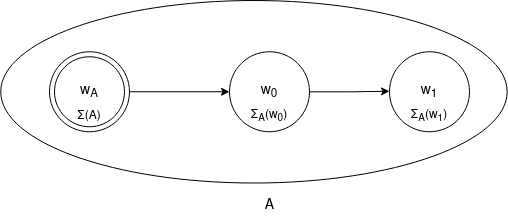
\includegraphics[scale=.5]{Figuras/Modelo.png}
                    \caption[Modelo Etiquetado]{Um exemplo de um modelo etiquetado chamado \(A\), onde \(w_A\) é seu mundo base}
                    \small{Fonte: \me}
                    \label{fig:ModeloEtiquetado}
                \end{figure}

                Considerando, para qualquer mundo \(w_j\) em \Modeloinicial, os conjuntos \(\funcao{S}_{\pi}(\Sigma_{\modeloinicial}(w_j))\)
                de \PI-átomos de \(\Sigma_{\modeloinicial}(w_j)\), esses conjuntos contém todos os elementos (fórmulas pertencentes à \(\Upsilon\)) de fórmulas em \(\Sigma_{\modeloinicial}(w_j)\).
                Estes conjuntos são chamados de \textit{conjuntos de concordância}, pois com base neles construiremos novos \OPImodelos etiquetados
                \Mathcal{N} cujo mundo base é \(w_j\) e que ``concordam'' com a valoração dos elementos dos conjuntos \(\funcao{S}_{\pi}(\Sigma_{\modeloinicial}(w_j))\).

                Para isso, chamaremos o conjunto
                \(\{\varsigma \ | \ \varsigma \in \funcao{S}_{\pi}(\Sigma_{\modeloinicial}(w_j))\} \cup \{\neg \varsigma \ | \ \varsigma \notin \funcao{S}_{\pi}(\Sigma_{\modeloinicial}(w_j))\}\)
                de elementos que são verdadeiros ou cuja negação é verdadeira em \(w_j\), de \textit{diagramas de concordância} e devemos garantir que estes conjuntos são
                \Mathcali{L}{12}-consistentes. Para garantir a consistência destes conjuntos, definimos os conjuntos
                \[
                    \funcao{T}_{\pi}(\Delta) = \{\Box^{n}_{\pi} \delta \ | \ \delta \in \funcao{B}(\funcao{S}_{\pi}(\Delta)) \cap \mathcal{L}_{12} \text{ e } d_\pi(\Box^{n}_{\pi} \delta) \leq d_\pi(\Delta) \}
                \]
                chamados de \PI-teorias e impomos a restrição que \(\funcao{T}_{\pi}(\funcao{S}_{\pi}(\Sigma(\modeloinicial)))\) deve ser verdadeiro em \Mundoinicial. A \PI-teoria
                de um dado conjunto \DDELTA é o conjunto de todos os \(\Box^{n}_{\pi}\text{-fechos}\) de teoremas que são componentes booleanos de fórmulas em \DDELTA, ou seja,
                é o conjunto de todas as fórmulas da forma \(\Box^{n}_{\pi} \phi\), tal que \(\phi\) é um teorema de \(\mathcal{L}_{12}\) e tem forma \(\neg \psi \text{ ou } \psi_0 \lor \psi_1\),
                e \textit{n} é menor ou igual ao comprimento da maior sequência de modalidades \BOXi{\pi} de alguma fórmula no conjunto \DDELTA.
                Como \GAMMA é \Mathcali{L}{12}-consistente e \(\funcao{T}_{\pi}(\funcao{S}_{\pi}(\Sigma(\modeloinicial))) \subseteq \mathcal{L}_{12}\),
                \(\Gamma \cup T_\pi(\funcao{S}_{\pi}(\Sigma(\modeloinicial)))\) é \Mathcali{L}{12}-consistente.
                % Esta é uma operação de seleção de \PI-átomos na definição de \PI-teorias que não é estritamente necessária para
                % provar a transferência de completude, porém permitem provar a transferência de outras propriedades.

                Para cada mundo \(w_j\) no conjunto de mundos de \Modeloinicial, o diagrama de concordância de \(w_j\) é \Mathcali{L}{12}-consistente e está contido em \(\Theta\),
                logo, existe um \OPImodelo etiquetado \Mathcal{N} baseado num frame para \Mathcali{L}{{\overline{\pi}}} que torna este diagrama verdadeiro em algum mundo. Chamaremos de \(w_x\)
                este mundo de \Mathcal{N}, tomaremos ele como o mundo base para \Mathcal{N} e assumimos que este é o único mundo que \Modeloinicial e \Mathcal{N} compartilham.
                O conjunto de elementos de \Mathcal{N} é o conjunto \(\funcao{S}_{\pi}(\Sigma_{\modeloinicial}(w_x))\), que é o conjunto concordância de \(w_x\). Por fim,
                \Mathcal{N} deve tornar a \OPI-teoria de \(\Sigma(\mathcal{N}) = \funcao{T}_{\overline{\pi}}(\funcao{S}_{\overline{\pi}}(\Sigma(\modeloinicial)))\), verdadeira em \(w_{\mathcal{N}}\).

                \begin{figure}[htbp]
                    \centering
                    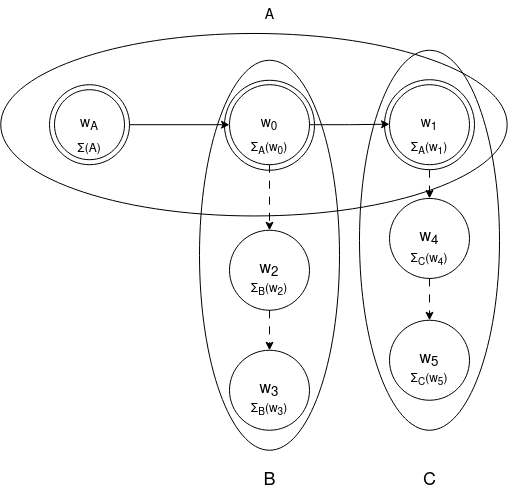
\includegraphics[scale=.5]{Figuras/MultiplosModelos.png}
                    \caption[Modelos Ancorados]{Modelos ancorados em \textit{A}, onde \textit{B} e \textit{C} são do tipo diferente que \textit{A},
                    \(w_0\) é o mundo base de \textit{B} e \(w_1\) é o mundo base de \textit{C}}
                    \small{Fonte: \me}
                    \label{fig:ModelosAncorados}
                \end{figure}

                Caso todas estas condições sejam satisfeitas, \Mathcal{N} é dito \textit{ancorado em} \Modeloinicial no mundo \(w_x\). Ancoramos em \Modeloinicial \OPImodelos etiquetados
                disjuntos (ou seja, que não compartilham mundos entre si) em cada mundo do modelo. Então, cada mundo de \Modeloinicial é o mundo base de algum
                \OPImodelo etiquetado ancorado em \Modeloinicial. Adicionalmente, podemos ancorar \PImodelos etiquetados nos \OPImodelos, ancorados em \Modeloinicial, em mundos que não são base.
                Esta construção pode ser repetida infinitamente. É importante ressaltar que, exceto o modelo etiquetado ancorado em \Mundoinicial em \Modeloinicial,
                nenhum modelo etiquetado será ancorado no mundo base de outro modelo etiquetado. Também é importante ressaltar que modelos etiquetados de um tipo só são ancorados em
                modelos etiquetados de outro tipo, ou seja, \PImodelos etiquetados só são ancorados em \OPImodelos etiquetados, e vice versa.

                Essa relação de ancoramento constrói uma árvore de modelos, onde a raiz é \Modeloinicial e novas folhas são inseridas ancorando modelos em algum modelo folha
                da árvore. Para então avaliar uma fórmula, devemos percorrer a árvore avaliando as subfórmulas da fórmula em modelos compatíveis com a fórmula\footnote{Ou seja, caso
                a fórmula seja do tipo \(\Box_{1}\phi\) ela é avaliada em um 1-modelo e caso a fórmula seja do tipo \(\Box_{2}\phi\) ela é avaliada em um 2-modelo.}.
                Logo, temos uma forma de avaliar, passo a passo, fórmulas que contenham modalidades distintas. Para então construir um 12-modelo que satisfaça o conjunto \GAMMA,
                devemos considerar 1- e 2-modelos ancorados uns nos outros que satisfazem as fórmulas \(\gamma \in \Gamma\). O conjunto de todo conjunto de modelos
                que satisfaz as fórmulas em \GAMMA será chamado de conjunto de \textit{brotos} de \Modeloinicial.

                O lema de Zorn~\cite{zorn1935remark} nos diz que o conjunto de brotos tem um elemento máximo. A união dos elementos (mundos, relações entre mundos e valorações) do elemento
                máximo do conjunto de brotos nos dará o 12-modelo desejado, do qual podemos obter um 12-frame para \Mathcali{L}{12}. Isso quer dizer que, na árvore de modelos gerada
                pela relação de ancoramento, existirá um caminho (sequência de modelos) que satisfaz todas as fórmulas do conjunto \GAMMA, podemos então unir todos os modelos deste caminho
                em um único modelo, do qual podemos obter um frame para \Mathcali{L}{12}.

                \begin{figure}[htbp]
                    \centering
                    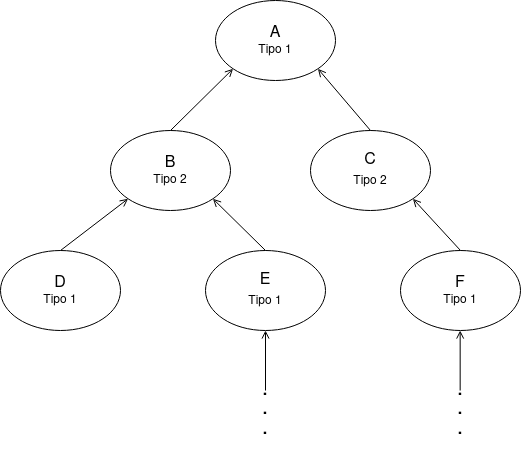
\includegraphics[scale=.5]{Figuras/ArvoreModelos.png}
                    \caption[Árvore de modelos]{Árvore de modelos com raiz em \(A\), onde uma seta indica um ancoramento}
                    \small{Fonte: \me}
                    \label{fig:ArvoreModelos}
                \end{figure}

                Isso conclui a prova informal do Teorema~\ref*{teo:TransCompletude}.
            \end{proof}

            A prova formal do Teorema~\ref{teo:TransCompletude} encontra-se no apêndice~\ref{app:ProvaTransferenciaCompletude}.

            % \begin{exemplo}[Valorando fórmulas em Modelos Ancorados]
            %     ESTE EXEMPLO TALVEZ NÃO ESTEJA CERTO !!!!
            %     Considerando a fórmula \PHI utilizada no Exemplo~\ref{exe:AplicacaoFuncao}:
            %     \[
            %         \phi = \Box_1 (p_0 \lor p_1) \to \Box_2 (p_3 \land (\Box_1 p_0 \lor \Box_2 p_1))
            %     \]
            %     Para valorar \PHI em um mundo \textit{w} de um 1-modelo etiquetado \textit{M}, devemos avaliar as subfórmulas \(\phi_1 = \Box_1 (p_0 \lor p_1)\) e
            %     \(\phi_2 =\Box_2 (p_3 \land (\Box_1 p_0 \lor \Box_2 p_1))\) em \textit{w}. \(\phi_1\) pode ser valorado em \textit{w}, porém \(\phi_2\) deve ser valorado em um 2-modelo
            %     etiquetado \textit{N} ancorado em \textit{M} no mundo \textit{w}. Considerando as subfórmulas \(\phi_3 = \Box_1 p_0\) e \(\phi_4 = \Box_2 p_1\) que devem ser valoradas em \textit{N},
            %     \(\phi_3\) deve ser valorado em um 1-modelo etiquetado \textit{I}, ancorado em \textit{N} em algum mundo \textit{x} tal que \(w \mathcal{R} x\), Já
            %     \(\phi_4\) pode ser valorado em \textit{N}. \qed
            % \end{exemplo}

            \begin{teorema}[Transferência de Completude Forte]
                \label{teo:TransCompletudeForte}
                Sendo \Mathcali{L}{1} e \Mathcali{L}{2} lógicas modais fortemente completas com relação às classes de frames \Mathfraki{F}{1} e \Mathfraki{F}{2},
                então \(\mathcal{L}_{12} = \mathcal{L}_{1} \Odot \mathcal{L}_{2}\) será fortemente completa com relação a classe de frames \(\mathfrak{F}_{12} = \mathfrak{F}_1 \Otimes \mathfrak{F}_2\).
            \end{teorema}

            \begin{proof}[Prova do Teorema~\ref{teo:TransCompletudeForte}]
                Completude forte é exatamente completude generalizada com relação ao espaço de fórmulas \(\mathsf{LM}_{12}\). No enunciado do Teorema~\ref{teo:TransCompletude},
                tome \(\Theta := \mathsf{LM}_{12}\), assim, \(\funcao{DC}_1(\mathsf{LM}_{12}) = \funcao{DC}_2(\mathsf{LM}_{12}) = \mathsf{LM}_{12}\), logo, pelo
                Teorema~\ref{teo:TransCompletude}, provamos o Teorema~\ref{teo:TransCompletudeForte}.
            \end{proof}

            \begin{teorema}[Transferência de Completude Fraca]
                \label{teo:TransCompletudeFraca}
                Sendo \Mathcali{L}{1} e \Mathcali{L}{2} lógicas modais fracamente completas com relação as classes de frames \Mathfraki{F}{1} e \Mathfraki{F}{2},
                \(\mathcal{L}_{12} = \mathcal{L}_{1} \Odot \mathcal{L}_{2}\) será fracamente completa com relação a classe de frames \(\mathfrak{F}_{12} = \mathfrak{F}_1 \Otimes \mathfrak{F}_2\).
            \end{teorema}

            \begin{proof}[Prova do Teorema~\ref{teo:TransCompletudeFraca}]
                Completude fraca é exatamente completude com relação à todo conjunto \(\{\phi\}\) onde \(\phi \in \mathsf{LM}_{12}\). Considerando um \PHI qualquer, no
                enunciado do Teorema~\ref{teo:TransCompletude}, tome \(\Theta = \funcao{B}(\funcao{Sub}(\phi))\). Como o conjunto definido por \(\funcao{Sub}(\phi)\) é finito por
                definição, \(\Theta = \funcao{B}(\funcao{Sub}(\phi))\) contém uma quantidade finita de formulas cujo valor verdade é diferente entre si\footnote{Veja Definição~\ref{def:FuncoesElementos}.}.
                Portanto, existe uma quantidade finita de fórmulas em \(\funcao{DC}_\pi(\Theta)\) que não são equivalente entre si em (um frame/modelo qualquer para) \(\mathcal{L}_\pi\).
                Então, todo subconjunto \(\Delta \subseteq \funcao{DC}_\pi(\Theta)\) é equivalente em (um frame/modelo qualquer para) \(\mathcal{L}_\pi\) a um conjunto de fórmulas finito
                \(\Delta_f\) e, portanto, é equivalente em (um frame/modelo qualquer para) \(\mathcal{L}_\pi\) a uma única fórmula (por exemplo \(\bigwedge \Delta_f\)), que será
                verdadeira no mundo \Mundoinicial no modelo \Modeloinicial, pela Definição~\ref{def:Definicao1}.

                Portanto, \Mathcali{L}{\pi} é completo com relação a \(\funcao{DC}_\pi(\Theta)\), logo, pelo Teorema~\ref{teo:TransCompletude}, \Mathcali{L}{12} é completa
                com relação a \(\Theta\) e, portanto, é completo com relação a \(\{\phi\}\).
            \end{proof}

            Este método de prova é suficientemente genérico para provar a transferência de outras propriedades, sendo necessário apenas pequenas variações em
            em componentes da prova, como demonstrado em~\citeshort{fine1996transfer}.

    \section{O Sistema Bimodal \texorpdfstring{\SisT}{T4}}
        \label{sec:SistemaKT4}
        O sistema bimodal \SisT é talvez um dos sistemas multimodais mais simples, ele consiste da fusão dos sistemas monomodais \textbf{KT} e \textbf{K4}.
        Este sistema será descrito formalmente nesta seção, pois foi usado como estudo de caso para a modelagem de fusão de lógicas modais em Coq, na biblioteca
        descrita no Capítulo~\ref{cap:Implementacao}.

        \subsection{Linguagem, Semântica e Axiomatização}
            \label{subsec:KT4LinguagemSemantica}
            A linguagem \linguagem{\mathcal{T}{4}} do sistema \SisT é baseada na assinatura \({\mathsf{C} = \{\Box_{T}, \Diamond_{T}, \Box_{4}, \Diamond_{4}, \neg, \land, \lor, \to\}}\)
            e é definida abaixo:

            \begin{definicao}[Linguagem de \SisT]
                A linguagem do sistema é \SisT definida indutivamente como o menor conjunto que satisfaz as seguintes regras:
                \begin{align*}
                    & \top, \bot \in \Linguagem{\mathcal{T}{4}}  \\
                    & \mathbb{P} \subseteq \Linguagem{\mathcal{T}{4}} \\
                    & \text{Se } \phi \in \Linguagem{\mathcal{T}{4}} \text{, então } \circ \phi \in \Linguagem{\mathcal{T}{4}}, \circ \in \{\Box_{T}, \Box_{4}, \Diamond_{T}, \Diamond_{4}, \neg\} \\
                    & \text{Se } \phi, \psi \in \Linguagem{\mathcal{T}{4}} \text{, então } \phi \circ \psi \in \Linguagem{\mathcal{T}{4}}, \circ \in \{\land, \lor, \to\} \tag*\qed
                \end{align*}
            \end{definicao}

            \begin{definicao}[\(\mathcal{T}{4}\)-frames e \(\mathcal{T}{4}\)-modelos]
                Um \(\mathcal{T}{4}\)-frame é uma tripla da forma \(\mathcal{F}_{\mathcal{T}{4}} = \langle \mathcal{W}, \mathcal{R}_{\mathcal{T}}, \mathcal{R}_{4} \rangle\),
                onde \(\mathcal{W} \neq \emptyset\), \(\mathcal{R}_{\mathcal{T}}, \mathcal{R}_4 \subseteq \mathcal{W} \times \mathcal{W}\) e \(\mathcal{R}_{\mathcal{T}}\) é uma
                relação reflexiva e \(\mathcal{R}_{4}\) é uma relação transitiva.

                Um \(\mathcal{T}{4}\)-modelo é um par da forma \(\mathcal{M}_{\mathcal{T}{4}} = \langle \mathcal{F}_{\mathcal{T}{4}}, \mathcal{V} \rangle\), onde
                \(\mathcal{V}: \mathbb{P} \to 2^{\mathcal{W}}\) e \(\mathcal{F}_{\mathcal{T}{4}}\) é um \(\mathcal{T}{4}\)-frame. \qed
            \end{definicao}

            \begin{definicao}[Valoração de Fórmulas]
                A valoração de fórmulas em \SisT é definida de forma igual à valoração de fórmulas para lógicas monomodais, com os casos para \BOX e \DIA substituídos por:
                \begin{align*}
                    \mathcal{M}_{\mathcal{T}{4}}, w_0 & \Vdash \Box_{T} \phi \text{ sse } \forall w_1 \in \mathcal{W}, (w_0 \mathcal{R}_{T} w_1 \to
                                    \mathcal{M}_{\mathcal{T}{4}}, w_1 \Vdash \phi)\\
                    \mathcal{M}_{\mathcal{T}{4}}, w_0 & \Vdash \Diamond_{T} \phi \text{ sse } \exists w_1 \in \mathcal{W}, (w_0 \mathcal{R}_{T} w_1 \land
                                    \mathcal{M}_{\mathcal{T}{4}}, w_1 \Vdash \phi)\\
                    \mathcal{M}_{\mathcal{T}{4}}, w_0 & \Vdash \Box_{4} \phi \text{ sse } \forall w_1 \in \mathcal{W}, (w_0 \mathcal{R}_{4} w_1 \to
                                    \mathcal{M}_{\mathcal{T}{4}}, w_1 \Vdash \phi)\\
                    \mathcal{M}_{\mathcal{T}{4}}, w_0 & \Vdash \Diamond_{4} \phi \text{ sse } \exists w_1 \in \mathcal{W}, (w_0 \mathcal{R}_{4} w_1 \land
                                    \mathcal{M}_{\mathcal{T}{4}}, w_1 \Vdash \phi) \tag*\qed
                \end{align*}
            \end{definicao}

            Outros conceitos semânticos são definidos de maneira análoga.

            \begin{definicao}[Axiomatização de \SisT]
                O conjunto de axiomas \(\Lambda_{\mathsf{LM}_{\mathcal{T}{4}}}\) para o sistema \SisT é uma especificação do conjunto \(\Lambda_{\mathsf{LM}_{n}}\) multimodal,
                onde as \textit{n} instâncias do axioma \(K_i\) são substituídas por:
                \begin{align*}
                    & \Box_T (p_0 \to p_1) \to (\Box_T p_0 \to \Box_T p_1) \tag{\(K_T\)} \\
                    & \Box_4 (p_0 \to p_1) \to (\Box_4 p_0 \to \Box_4 p_1) \tag{\(K_4\)}
                \end{align*}
                e com a adição dos axiomas \textit{T}:
                \[
                    \Box_T \phi \rightarrow \phi
                \]
                e \textit{4}:
                \[
                    \Box_4 \phi \to \Box_4 \Box_4 \phi
                \]
                O conjunto de regras de derivação é definido como \(\mathfrak{R} = \{\textit{Nec}_T, \textit{Nec}_4, \textit{MP}\}\).
                Logo, o sistema \SisT pode ser axiomatizada pelo par
                \(\langle\Lambda_{\mathsf{LM}_{\mathcal{T}{4}}}, \{\textit{Nec}_T, \textit{Nec}_4, \textit{MP}\}\rangle\). \qed
            \end{definicao}

        \subsection{Corretude e Completude}
            \label{subsec:KT4CorretudeCompletude}
            Como demonstrado por~\citeauthoronline{blackburn2001modal} (\citeyear{blackburn2001modal}), os sistemas monomodais \textbf{KT} e \textbf{K4} são ambos corretos e fortemente completos, sendo \textbf{KT} correto e fortemente completo
            para a classe \(\mathfrak{F}_{\mathcal{T}}\) de frames reflexivos e sendo \textbf{K4} correto e fortemente completo para a classe \(\mathfrak{F}_{4}\) de frames transitivos.
            Portanto, pelos Teoremas~\ref{teo:TransCorretude} e~\ref{teo:TransCompletudeForte}, temos que o sistema \SisT é correto e fortemente completo para a classe
            \(\mathfrak{F}_{\mathcal{T}4}\) de 2-frames da forma \(\langle \mathcal{W}, \mathcal{R}_{\mathcal{T}}, \mathcal{R}_{4} \rangle\), sendo \(\mathcal{R}_{\mathcal{T}}\) uma relação
            reflexiva e \(\mathcal{R}_{4}\) uma relação transitiva.
\chapter{Assistentes de Provas}
	\label{cap:AssistentesProvas}
	Segundo~\citeshort{geuvers2009proof}, assistentes de provas\footnote{Também chamados de provadores semi-automáticos de teoremas ou provadores interativos.}
	são sistemas computacionais que permitem usuários definirem, provarem propriedades e
	raciocinarem sobre teorias e objetos matemáticos.~\citeshort{harrison2014history} descrevem como um sistema que um humano usa interativamente para produzir
	provas formais. Já~\citeshort{silva2019certificacao} descreve como programas que auxiliam no desenvolvimento de provas formais, mas não as fazem automaticamente e
	necessitam de um humano para guiar a prova.

	Segundo~\citeshort{harrison2014history} o conceito de assistentes de provas surge durante os anos de 1960 e 1970, a partir do reconhecimento que a capacidade de provadores
	automáticos de teoremas estavam estagnando, apesar de grande atividade e inovação na área. Provadores automáticos de teoremas, ao contrário de assistentes de provas,
	são softwares que automaticamente geram, se possível, provas para expressões matemáticas, geralmente por um método de busca em um domínio específico.
	De acordo com~\citeshort{harrison2014history} e~\citeshort{geuvers2009proof}, durante este período surgiram os primeiros assistentes de provas, dentre eles estão Automath, LCF, Mizar e PVS.

	De acordo com~\citeshort{silva2019certificacao}, provas assistidas por computador inicialmente não foram bem recebidas pela comunidade matemática, pois o objetivo de uma prova é
	convencer um leitor que algo é verdadeiro e explicar o porquê, algo que provas desenvolvidas em computador não são bem adaptadas, pois, em geral,
	suas linguagens internas não são de fácil entendimento. Porém, diversos resultados importantes foram provados em assistentes de provas, segundo~\citeshort{geuvers2009proof},
	o teorema da Curva de Jordan foi provado em ambos Mizar e HOL Light, o Teorema dos Números Primos foi provado em Isabelle e o Teorema das Quatro Cores foi provado em Coq.

	É de interesse analisar mais este último teorema, pois foi o primeiro grande resultado provado em um computador. Em específico, o problema foi detalhado e alguns casos foram provados
	em~\citeshort{appel1976every} e outros casos, além de uma prova em computador (em linguagem \textit{assembly} para computadores IBM 370), foi apresentada em~\citeshort{appel1977every}.
	O motivo da prova ter sido realizada em um computador é devido à quantidade de casos a serem analisados, cerca de 1 bilhão de acordo com~\citeshort{gonthier2005computer}.

	A prova de~\citeauthoronline{appel1977every} não foi imediatamente aceita pela comunidade matemática, apenas com a publicação de uma monografia definitiva da prova
	em~\citeshort{appel1989every} e com a prova de~\citeshort{robertson1997four}, também em computador mas muito mais simples e feita na linguagem C, o Teorema
	das Quatro Cores foi considerado provado~\cite{gonthier2005computer}. Por fim,~\citeshort{gonthier2005computer} formalizou a prova de~\citeauthoronline{robertson1997four} em Coq, dando,
	o que o autor descreve, como o passo final na prova. Ao longo dos anos, provas formalizadas em computador conseguiram reconhecimento, pois se
	demonstraram mais confiáveis que provas tradicionais.

	Assistentes de provas também são amplamente usados para verificar componentes de software, segundo~\citeshort{avigad2017theorem} \textit{verificação formal}
	consiste no uso de métodos matemáticos e computacionais para expressar afirmações em termos matemáticos precisos. Essas afirmações podem se referir à corretude
	de certos sistemas de software ou hardware ou à garantia de que um certo estado de um programa nunca será atingido, estes que, ao serem expressos em termos matemáticos,
	podem ser demonstrados por meio de assistentes de provas.

	Segundo~\citeshort{silva2019certificacao}, assistentes de provas tem propriedades interessantes, por exemplo, verificação rápida e mecânica de provas,
	comandos de busca de teoremas e lemas e automatização de provas. Uma propriedade que alguns assistentes de provas compartilham
	(por exemplo Coq~\cite{coqteam2022manual} e Lean~\cite{avigad2017theorem,demoura2015lean}) é satisfazer critério de de Bruijn. O critério afirma que o programa
	verificador de um assistente (seu \textit{kernel} ou \textit{núcleo}) deve ser um programa muito pequeno, que pode ser verificado manualmente, seja por meio de papel e caneta ou por
	um algoritmo simples que uma pessoa cética poderia desenvolver facilmente~\cite{barendregt2001proof}. O verificador deve gerar algum tipo de ``objeto de prova'',
	por exemplo um termo \(\lambda\), que pode ter sua veracidade comprovada da mesma forma que o verificador de tipos.

	Neste capítulo, será apresentado o conceito de teoria de tipos e o assistente de provas Coq será descrito. Na Seção~\ref{sec:TeoriaTipos} será
	brevemente apresentada a Teoria de Tipos e na Seção~\ref{sec:Coq} será descrito o assistente de provas Coq.

	\section{Uma Breve Apresentação de Teoria de Tipos}
		\label{sec:TeoriaTipos}
		Teoria dos tipos surge, de acordo com~\citeshort{sep-type-theory}, como uma tentativa de Russell para lidar com o Paradoxo de Russell:
		sendo \(R = \{ x \ | \ x \notin x\}\) então \( R \in R \tofrom R \notin R\), presente na Teoria de Conjuntos.
		O cerne do paradoxo se encontra na quantificação de \textit{x} na definição de \textit{R}, em específico, \textit{x} é quantificado sobre
		todos os conjuntos, o que inclui o próprio conjunto \textit{R}, possibilitando então que \textit{x} seja instanciado como \textit{R}.

		Em uma carta para Frege escrita em 1902, Russell comunica a descoberta do paradoxo e indica que o problema está relacionado com a quantificação
		de objetos; Frege responde à Russell menos de uma semana depois, indicando que uma possível solução para o problema lidaria com ``níveis'' de objetos,
		assim impedindo que um objeto de um dado nível possa quantificar sobre objetos de níveis diferentes~\cite{van2002frege}. Porém, uma proposta de solução ao paradoxo
		surge apenas no apêndice B de~\citeshort{russell1903principles}\footnote{É de interesse ressaltar a seguinte passagem do livro, presente no Apêndice A,
		página 762: ``\textit{A variable will not be able, except in special cases, to extend from one of these sets into another; and in \(x \in u\), the
		x and the u must always belong to different types}[...]''.} onde Russell introduz provisoriamente a ``Doutrina de Tipos'',
		o que eventualmente se tornou a Teoria de Tipos moderna.

		Após explorar diversas outras teorias para lidar com os paradoxos da Teoria de Conjuntos~\cite{van2002frege}, Russell voltou a trabalhar
		na teoria de tipos, resultando na Teoria de Tipos Ramificada~\cite{russell1908mathematical}. Porém, problemas presentes nesta
		teoria\footnote{Para mais detalhes sobre, veja~\cite[p. 150-153]{van2002frege}.} levaram \citeshort{ramsey1931general} a desenvolver
		a Teoria de Tipos Simples, que é uma versão mais restrita da Teoria de Tipos Ramificada.

		A Teoria de Tipos Simples foi reformulada por Church~\cite{church1940formulation} para desenvolver a sua própria versão da teoria de
		tipos, usando a sintaxe do \CalcLambda, o que hoje é chamado de \CLST~\cite{huet1990logical}. Na sua formulação, novos tipos
		são definidos indutivamente a partir de dois tipos básicos, (\textit{i} para indivíduos e \textit{o} para proposições) e de uma regra
		de definição de tipos (sendo \textit{A} e \textit{B} tipos, então toda função \(A \to B\) de \textit{A} para \textit{B} é um tipo).
		Predicados tem tipo \(i \to o\) e funções tem tipo \(i \to i\). Por fim, expressões são definidas a partir de uma linguagem de \CalcLambda estendida para
		lidar com tipos.

		Segundo~\citeshort{howard1980formulae},~\citeshort{curry1958combinatory} apontaram uma correspondência direta entre axiomas do fragmento positivo implicativo
		de lógica proposicional e combinadores do \CalcLambda, já~\citeshort{tait1967intensional} observou uma correspondência direta entre a regra de eliminação do corte
		em Cálculo de Sequentes e redução de Termos \(\lambda\). \citeshort{howard1980formulae} então demonstrou, com base nestes resultados, que há uma
		correspondência direta entre a Lógica Intuicionista (descrita sintaticamente como um cálculo de sequentes) e o \CalcLambda Simplesmente Tipado,
		dando surgimento ao que hoje é chamado de Correspondência de Curry-Howard\footnote{Essa noção é expandida por Wadler~\cite{wadler2015propositions}
		onde o autor defende que a Correspondência é apenas um nome para um fenômeno maior chamado de \textit{Propositions as Types}
		(Proposições como Tipos).}.

		Na década de 1970 foi desenvolvido um novo tipo de \CalcLambda tipado, chamado de Sistema F ou \CalcLambda de Segunda Ordem, independentemente por~\citeshort{girard1971extension}
		e~\citeshort{reynolds1974towards}. Este sistema estende o \CLST adicionando uma operação de abstração de tipos, permitindo definir termos \(\lambda\)
		com variáveis que podem ser instanciadas como um tipo~\cite{girard1989proofs}. Isso se mostrou especialmente útil para a computação, em específico
		para a formalização do conceito de funções polimórficas.

		Pouco tempo após o desenvolvimento do Sistema F,~\citeauthoronline{girard1972interpretation} apresentou o Sistema \(\mathrm{F}_\omega\)~\cite{girard1972interpretation}
		que é uma generalização do Sistema F, adicionando os conceitos de construtores de tipos e \textit{kinds}\footnote{Pode ser traduzido como ``gênero''.}.
		Construtores de tipos são tipos especiais de funções que recebem tipos e retornam tipos, já \textit{kinds} podem ser entendidos como ``tipos de tipos'',
		essencialmente é uma cópia do \CLST a nível de tipos~\cite{pierce2002types}. As abstrações de tipos do Sistema F pode ser entendida
		como uma dependência de termos em tipos, já os construtores de tipos do Sistema \(\mathrm{F}_\omega\) pode ser entendidos como uma dependência
		entre tipos.

		Outro importante desenvolvimento na teoria de tipos foi a Teoria de Tipos Intuicionista ou Teoria de Tipos de Martin-Löf~\cite{martin1975intuitionistic,martin1984intuitionistic},
		proposta por~\citeauthoronline{martin1975intuitionistic} como um sistema lógico fundacional para a matemática construtivista, de forma análoga à
		Teoria de Conjuntos de Zermelo-Frankel para a matemática clássica. Uma das características deste sistema é uma distinção rigorosa entre proposições
		e julgamentos; proposições são objetos que podem ser combinados por meio de operações lógicas como \(\neg, \land, \lor, \to, \exists, \forall\), já
		julgamentos são afirmações sobre proposições. Por exemplo, na frase ``\PHI é verdadeiro'', \PHI é uma proposição e ``\PHI é verdadeiro'' é um
		julgamento~\cite{martin1984intuitionistic}.

		A \TTML está intimamente relacionada à \CCH, pois toda proposição em \TTML representa um tipo, o tipo de todas as provas da proposição. Por exemplo,
		a frase ``971 é um número não primo'' descreve a proposição que é provada fornecendo dois números naturais maiores que 1 e uma computação que mostra
		que seu produto é 971. Por outro lado, todo tipo também descreve uma proposição, em específico, a proposição que o tipo em questão não é vazio, que
		é provada fornecendo um objeto que habita o tipo~\cite{martin1975intuitionistic}. Ao provar uma proposição em \TTML, construímos um objeto que habita o tipo
		desta proposição, estes objetos são chamados de \textit{objetos de prova} e são ditos serem \textit{testemunhas} para a verdade da proposição~\cite{sep-type-theory-intuitionistic}.

		Duas noções importantes para a Teoria de Tipos são introduzidas na \TTML, são elas o Universo de Tipos e Tipos Dependentes. Universo de tipos é uma forma de lidar
		com a necessidade de criar tipos arbitrários dentro da linguagem. Existem duas famílias de tipos: os tipos pequenos e os tipos grandes, estas respeitam
		a seguinte hierarquia bem fundada: \(V_0 \in V_1 \in V_2 \in \dots \in V_n \in \dots\)\footnote{Aqui considere que a notação \(a \in B\) indica que \textit{B}
		é o tipo do objeto \textit{a}.}, sendo \(V_0\) a família dos tipos pequenos e toda família \(V_i, i \geq 1\) dos tipos grandes
		de ordem \textit{i}, onde todo \(V_n\) tem tipo \(V_{n+1}\)~\cite{martin1975intuitionistic}. É importante ressaltar que não é possível impor a restrição
		que um tipo seja um objeto dele mesmo, ou seja que \textit{V} tenha tipo \textit{V}, pois isso levaria a uma contradição semelhante ao Paradoxo de Russell~\cite{girard1972interpretation}.
		Uma variável de tipo em uma expressão é dita dependente se o tipo a qual ela será instanciada depende do valor de algum termo na expressão, nesse
		caso o tipo de toda a expressão é dito dependente~\cite{martin1975intuitionistic}.
		% Por exemplo, um predicado \(\mathrm{Primo}(x)\) que representa se o número
		% \textit{x} é ou não primo, depende do valor de \textit{x}, pois, caso \textit{x} seja um número primo, \(\mathrm{Primo}(x)\) será o tipo de provas
		% de que \textit{x} é primo, caso \textit{x} não seja primo, \(\mathrm{Primo}(x)\) será o tipo vazio.

		Segundo~\citeshort{coqteam2022manual},~\citeauthoronline{coquand1985constructions} uniram o sistema \(\mathrm{F}_\omega\) e a \TTML para criar o Cálculo de Construções (CoC),
		que é um sistema lógico baseado em teoria de tipos intuicionista com abstrações de tipos, construtores de tipos e tipos dependentes capaz de
		descrever indiretamente definições indutivas. Mais ainda, segundo~\citeshort{paulinmohring2015introduction}, o Cálculo de Construções é um sistema de tipos
		puro, ou seja, é um tipo de \CalcLambda com uma única linguagem que descreve ambos tipos e termos.

		Na Figura~\ref{fig:CuboLambda}, é apresentado um diagrama proposto originalmente por~\citeshort{barendregt1991introduction} para demonstrar relações entre
		diversos sistemas de tipos modernos. Cada flecha indica uma relação de inclusão (\(\subseteq\)) entre seus vértices, ou seja, o vértice de origem de uma flecha está incluso
		no vértice de destino da mesma. Uma das principais ideias no diagrama é representar as possíveis dependências mútuas entre tipos e termos, da seguinte forma:

		\begin{itemize}
			\item Tipos dependerem de termos (\(\rightarrow\))
			\item Termos dependerem de tipos (\(\uparrow\))
			\item Tipos dependerem de tipos (\(\nearrow\))
		\end{itemize}

		Como termos dependerem de outros termos é um componente básico do \CalcLambda, isso não é representado. Os sistemas de tipos representados são os seguintes:

		\begin{itemize}
			\item \(\lambda{\to}\): \CLST;
			\item \(\lambda 2\): Sistema F;
			\item \(\lambda\omega\): Sistema \(\mathrm{F}_{\omega}\);
			\begin{itemize}
				\item \(\lambda\underline{\omega}\): Uma versão mais fraca do Sistema \(\mathrm{F}_{\omega}\);
			\end{itemize}
			\item \(\lambda\Pi\): \textit{Logical Framework}, um sistema de \CalcLambda com tipos dependentes~\cite{harper1993framework};
			\item \(\lambda\mathrm{C}\): Cálculo de Construções.
		\end{itemize}

		\begin{figure}
			\centering
			\begin{tikzpicture}
				\matrix (m) [matrix of math nodes, row sep=3em, column sep=3em,
				text height=1.5ex,text depth=0.25ex]
				{
							& \lambda\omega             &              & \lambda\mathrm{C}            \\
				\lambda 2   &                           & \lambda\Pi 2                                \\
							& \lambda\underline{\omega} &              & \lambda\Pi\underline{\omega} \\
				\lambda{\to}&                           & \lambda\Pi  \\
				};
				\path[-{Latex[length=2.5mm, width=1.5mm]}]
				(m-1-2) edge (m-1-4)
				(m-2-1) edge (m-2-3)
						edge (m-1-2)
				(m-3-2) edge (m-1-2)
						edge (m-3-4)
				(m-4-1) edge (m-2-1)
						edge (m-3-2)
						edge (m-4-3)
				(m-3-4) edge (m-1-4)
				(m-2-3) edge (m-1-4)
				(m-4-3) edge (m-3-4)
						edge (m-2-3);
			\end{tikzpicture}
			\caption[Cubo \(\lambda\)]{Cubo \(\lambda\)\protect\footnotemark}
			\small{Fonte: Adaptado de~\cite{barendregt1991introduction}.}
			\label{fig:CuboLambda}
		\end{figure}
		\footnotetext{Diagrama originalmente produzido por Artem Pelenitsyn, de título original ``Lambda Cube'', gratuitamente disponível
		em \url{https://www.overleaf.com/latex/examples/lambda-cube/drnrtqnnjfzf}, licenciado pela licença Creative Commons CC BY 4.0 \url{https://creativecommons.org/licenses/by/4.0/deed.pt_BR}.}

		O Cálculo de Construções foi estendido por~\citeshort{coquand1988inductively} com a inclusão de definições indutivas primitivas, o que gerou o
		Cálculo de Construções Indutivas (CCI)~\cite{coqteam2022manual}. Este sistema de tipos é o formalismo por trás do Coq, todo objeto
		definido dentro do Coq é traduzido para um termo do CCI.

		Como apresentado em~\citeshort{coqteam2022manual}, no CCI, todo objeto tem um tipo, incluindo os próprios tipos.
		O tipo dos tipos se chama \textit{sort}\footnote{Pode ser traduzido adequadamente como ``classe''.}, e há uma hierarquia infinita e bem-fundada de \textit{sorts},
		onde os \textit{sorts} base são \textit{Set} e \textit{Prop}. Usaremos a notação \(A:\ B\) para denotar que o objeto \textit{A} tem tipo \textit{B}.

		O \textit{sort Set} é o tipo de todos os tipos pequenos, isto inclui tipos como o
		tipo dos números naturais e o tipo de termos booleanos, e também produtos, subconjuntos e funções sobre estes tipos. O \textit{sort Set} é o menor dos tipos.

		O \textit{sort Prop} é o tipo de proposições lógicas, onde um objeto \(\mathbb{P}: \textit{Prop}\) descreve uma classe de termos que representam
		provas de \Mathbb{P}, já um objeto \(\textit{p}: \mathbb{P}\) é dito uma \textit{testemunha} para a provabilidade da proposição \Mathbb{P}.
		Objetos em \textit{Prop} que não tem testemunhas são contradições.
		O \textit{sort SProp} é uma extensão do Coq originalmente proposta por \citeshort{gilbert2019definitional} que define uma classe de
		proposições estritas, estas são proposições cujas provas são irrelevantes (todas as provas são iguais).
		Ambos os \textit{sorts Prop} e \textit{SProp} são impredicativos, isto é, uma função que quantifica sobre todos os \textit{Props}/\textit{SProps} é
		também do tipo \textit{Prop}/\textit{SProp}. Formalmente, segundo~\citeshort{crosilla2017predicativity}, uma definição é impredicativa se define
		uma entidade por referência a alguma totalidade à qual a própria entidade pertence, e é predicativa caso contrário.

		Como \textit{Set} ser do tipo \textit{Set} gera uma teoria inconsistente, a linguagem do Cálculo de Construções Indutivas tem infinitos \textit{sorts}
		\(\textit{Type(i)}, i \geq 1\). Em particular, os \textit{sorts} \textit{Set}, \textit{Prop} e \textit{SProp} são do tipo \textit{Type(1)} e
		\(\forall i, \textit{Type(i)}: \textit{Type(i+1)}\). Os tipos são cumulativos, ou seja, para qualquer x, se \(x: \textit{Type(i)}\) então \(x: \textit{Type(i+1)}\),
		de forma análoga ao que ocorre na \TTML.

		% Uma característica importante do CCI são os tipos dependentes, que, segundo~\cite{pierce2002types}, podem ser entendidos como famílias de tipos que são
		% indexadas por termos, ou seja, o tipo de alguma expressão pode ser definido a partir do valor de algum termo.

	\section{O Assistente Coq}
		\label{sec:Coq}
		Coq é um assistente de provas para lógica de ordem superior desenvolvido desde 1984 por membros do instituto francês INRIA e seu \textit{kernel}
		é baseado no CCI. De acordo com~\citeshort{silva2019certificacao}, a Correspondência de Curry-Howard é o que
		dá versatilidade suficiente para o Coq para expressar lógicas mais sofisticadas, o autor ainda afirma que parte considerável
		da matemática pode ser expressa em Coq.

		Segundo~\citeshort{silva2019certificacao}, dentro da Ciência da Computação, Coq é usado principalmente como uma ferramenta para verificação de programas,
		como é o caso de~\citeshort{leroy2021compcert}, que desenvolveu um compilador para a linguagem C totalmente verificado em Coq, chamado de CompCert.
		Coq também pode ser usado para formalizar sistemas lógicos, como é o caso de~\citeshort{silveira2022sound} e~\citeshort{dewind2001modal} que descrevem a lógica modal alética
		em Coq e ~\citeshort{paiva1998temporal} que descreve a lógica temporal em Coq.

		De acordo com~\citeshort{silva2019certificacao}, Coq é tanto uma linguagem de programação funcional quanto uma linguagem de provas. Mais especificamente,
		Coq é composto dos seguintes componentes:
		\begin{itemize}
			\item \textit{Gallina}, que é uma linguagem de especificação e programação funcional, onde todo programa termina;
			\item \textit{Vernacular}, que é uma linguagem de comandos, permite interagir com o \textit{kernel} do Coq;
			\item Um conjunto de táticas para realizar provas, que são traduzidas para termos em \textit{Gallina};
			\item \Ltac, que é uma linguagem para implementação de táticas.
		\end{itemize}

		% Exemplos de provas / códigos
		Para utilizar o Coq de forma interativa, ferramentas como o CoqIDE\footnote{\url{https://coq.inria.fr/refman/practical-tools/coqide.html}.},
		VSCoq\footnote{\url{https://github.com/coq-community/vscoq}.} ou o ProofGeneral\footnote{\url{https://proofgeneral.github.io/}.} podem ser utilizadas.
		No que segue, serão apresentados exemplos feitos no CoqIDE, porém o mesmo se aplica às outras ferramentas.

		Para realizar uma prova em Coq usa-se os comandos \texttt{Theorem, Lemma, Example} ou \texttt{Corollary}\footnote{Internamente ao Coq todos são sinônimos, a
		distinção é apenas para os leitores.} para declarar uma expressão que será provada. Provas são iniciadas com o comando \texttt{Proof} e
		finalizadas com o comando \texttt{Qed} ou o comando \texttt{Defined}, mais ainda, provas podem ser aceitas sem serem completas com o comando
		\texttt{Admitted} e interrompidas com o comando \texttt{Abort}.

		Coq permite a definição indutiva de novos tipos, assim como a definição de funções recursivas e não recursivas. Tipos indutivos, definidos pelo comando
		\texttt{Inductive}, são definidos analogamente como na matemática ``tradicional'', onde é definido um conjunto de casos base para a indução e
		regras para a criação de novos objetos do tipo, onde ambos casos base e regras são chamados de construtores do tipo.
		Funções recursivas podem ser definidas pelo comando \texttt{Fixpoint}, estas operam sobre objetos de tipos indutivos podendo
		ter comportamentos diferentes dependendo de qual construtor de tipo foi usado para definir o objeto. Por fim, Coq também permite
		a definição de objetos arbitrários, com o comando \texttt{Definition}, que não passam da atribuição de um nome a algum termo~\cite{pierce2021software}.

		No desenvolvimento de provas interativas com o Coq uma prova pode ser verificada ``passo a passo'' pelo (\textit{kernel} do) Coq enquanto é desenvolvida (isto é, antes de
		ser finalizada). As ferramentas apresentadas anteriormente dispõem de duas janelas, uma janela de edição de texto,
		onde a prova de fato é escrita e uma janela de visualização, onde o estado da prova pode ser acompanhado, como pode ser visto com o caso do CoqIDE
		na Figura~\ref{fig:CoqIDEIntros}. O estado de uma prova é o conjunto de todas as hipóteses desta prova, assim como o conjunto de todos os termos que
		devem ser provados, chamados de \textit{goals} ou objetivos~\cite{coqteam2022manual}. O \textit{goal} pode ser separado em diversos \textit{subgoals}
		com a aplicação de algumas táticas, onde cada \textit{subgoal} deve ser provado para terminar a prova.
		A janela de visualização é dividida em duas partes por uma linha de inferência. Acima da linha estão as hipóteses e abaixo da linha está o \textit{goal},
		como pode ser visto na Figura~\ref{fig:CoqIDEIntros}.
		\begin{figure}[htpb!]
			\centering
			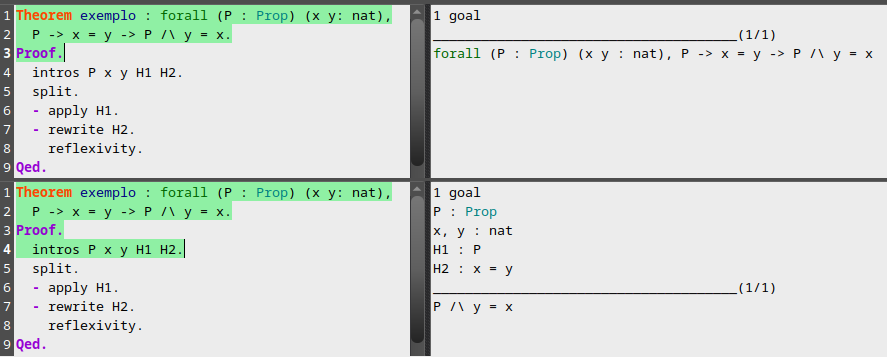
\includegraphics[scale=.5]{Figuras/CoqIDEIntrosJoin.png}
			\caption{Antes e depois de aplicar a tática \texttt{intros}.}
			\small{Fonte: \me}
			\label{fig:CoqIDEIntros}
		\end{figure}

		Durante o desenvolvimento interativo de provas, linhas são destacadas pela ferramenta que está sendo utilizada, a partir da resposta dada pelo verificador de tipos
		sobre o conteúdo daquela linha. Linhas destacadas em verde não geraram qualquer erro e foram aceitas pelo verificador de tipos, linhas destacadas em amarelo
		geraram algum tipo de aviso e linhas em vermelho foram rejeitadas pelo verificador de tipos, isto é, estão erradas de alguma forma.

		Na Figura~\ref{fig:CoqIDECores}, as linhas 13 e 15 até 17 estão destacas em amarelo pois não foram verificadas pelo verificador de tipos do Coq, isso é devido aos
		comandos \texttt{Admitted} e \texttt{Axiom}, que fazem com que os termos não sejam verificados pelo Coq e sejam tratados como verdades. A linha 23
		está destacada em vermelho pois ocorreu um erro nela, em específico, o Coq rejeitou a aplicação da tática \texttt{easy}. As restantes estão destacadas em verde
		pois foram aceitas pelo verificador de tipos.
		\begin{figure}[htpb!]
			\centering
			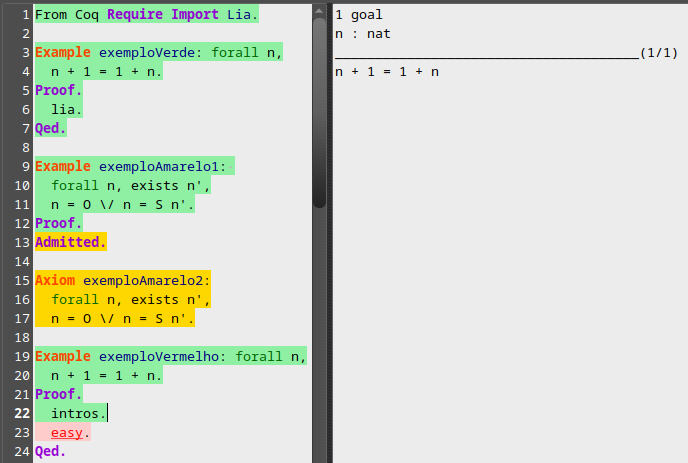
\includegraphics[scale=.5]{Figuras/CoqIDECores.png}
			\caption{Provas no CoqIDE.}
			\small{Fonte: \me}
			\label{fig:CoqIDECores}
		\end{figure}

		Dentro de provas no Coq, objetos são manipulados com táticas, por exemplo, a tática \texttt{intros} introduz termos quantificados universalmente
		no \textit{goal} e termos à esquerda de implicações\footnote{Estes na realidade são um caso particular de quantificação universal onde não há
		dependência de tipos entre o termo quantificado e a proposição sobre a qual ele está quantificado~\cite{pierce2021software}.} para o conjunto de hipóteses,
		a tática \texttt{apply} modifica o \textit{goal} ou as hipóteses com base no que está sendo aplicado e onde\footnote{Em específico, caso aplique-se um termo de tipo
		\(\texttt{A} \to \texttt{B}\) numa hipótese de tipo \texttt{A}, seus tipos serão unificados e a hipótese resultante terá tipo \texttt{B}, ou seja, equivale a aplicar
		a regra de modus ponens; caso aplique-se um termo de tipo \(\texttt{A} \to \texttt{B}\) num \textit{goal} de tipo \texttt{B}, seus tipos serão unificados e o
		\textit{goal} resultante terá tipo \texttt{A}, ou seja, é um tipo de \textit{backwards reasoning} - para provar \texttt{B} basta provar \texttt{A}.}
		e a tática \texttt{rewrite} reescreve equivalências no \textit{goal} ou em hipóteses.

		No que segue, conceitos de Coq serão apresentados por meio de exemplos práticos feitos pelo autor ou retirados de~\citeshort{pierce2021software}.

		\begin{exemplo}[Definições e Funções em Coq]
			Abaixo é definido indutivamente o tipo ``nat'' que representa os número naturais. Um número natural ou é \texttt{O} (representa o número 0) ou é o
			sucessor de outro número natural, representado como a aplicação da função sucessor \texttt{S} a algum número.
			A função recursiva ``plus'' apresenta a definição recursiva da soma de dois números naturais, já a função ``pred'' descreve uma operação de predecessor de um número.
			\begin{lstlisting}[language=coq]
		Inductive nat : Set :=
		  | O
		  | S: nat -> nat.
		Fixpoint plus (n : nat) (m : nat) : nat :=
		  match n with
		  | O => m
		  | S n' => S (plus n' m)
		  end.
		Definition pred (n : nat) : nat :=
		  match n with
		  | O => O
		  | S n' => n'
		  end.
			\end{lstlisting}
			Definições indutivas também podem ser utilizadas para descrever relações, como é o caso da relação ``ev'', representando paridade de números, abaixo.
			Esta definição descreve uma relação que associa números naturais (\texttt{nat}) à provas (\texttt{Prop}).
			\begin{lstlisting}[language=coq]
		Inductive ev : nat -> Prop :=
		  | ev_0 : ev 0
		  | ev_SS (n : nat) (H : ev n) : ev (S (S n)).
			\end{lstlisting}

			O construtor \texttt{ev\_SS} de \texttt{ev} requer \textit{evidências} para ser aplicado, em específico, ele requer um número natural \texttt{n} e uma prova
			\texttt{H} de \texttt{ev n}, ou seja, uma prova que \texttt{n} é par. Ao aplicar \texttt{ev\_SS} em algum termo, será necessário fornecer estas evidências
			para que verificador de tipos do Coq aceite a aplicação. \qed
		\end{exemplo}

		Para realizar provas em Coq, uma proposição é declarada, um nome é atribuído à ela e então um termo é construído a partir de axiomas,
		premissas e outros resultados já provados. Táticas são usadas para manipular estes e outros objetos relevantes para a prova até que esta seja concluída.
		Quando concluída, o termo provado é incluído no universo de fatos do Coq e pode ser utilizada em provas futuras.

		\begin{exemplo}[Provas em Coq]
			O teorema ``exemplo1'' mostra uma prova da comutatividade da disjunção lógica, já o lema ``exemplo2'' mostra uma prova indutiva que a soma de
			qualquer número natural com 0 é igual ao próprio número. Provas sobre relações indutivas podem ser feitas
			aplicando os construtores destas relações, no caso de \texttt{ev} do exemplo anterior, aplicando as regras \texttt{ev\_0} e \texttt{ev\_SS},
			como apresentado no corolário ``exemplo3'' abaixo, que prova que 4 é um número par.
			\begin{lstlisting}[language=coq]
		Theorem exemplo1: forall A B: Prop,
		  A \/ B -> B \/ A.
		Proof.
		  intros A B [HA | HB].
		  - right. assumption.
		  - left. assumption.
		Qed.
		Lemma exemplo2: forall n: nat,
		  n + 0 = n.
		Proof.
		  intros n.
		  induction n as [ | n' IHn].
		  - reflexivity.
		  - simpl. rewrite IHn. reflexivity.
		Qed.
		Corollary exemplo3: ev 4.
		Proof. apply ev_SS. apply ev_SS. apply ev_0. Qed.
			\end{lstlisting}
			\qed
		\end{exemplo}

		\subsection{Automação em Coq}
			\label{subsec:AutoCoq}
			Há diversos comando de automação em Coq, cujo intuito é agilizar o desenvolvimento de provas. Estes comandos se dividem em duas categorias,
			os \textit{tacticals} e as táticas de automação propriamente ditas. \textit{Tacticals} são ``táticas de ordem superior'', táticas que recebem
			outras táticas como argumento~\cite{pierce2021software}. Alguns dos comandos mais comuns são apresentados abaixo.

			\begin{exemplo}[\texttt{try}]
				O \textit{tatical} \texttt{try} tenta executar uma tática \Mathbb{T}, caso esta tenha sucesso, \Mathbb{T} é executada como normal, porém, caso
				\Mathbb{T} falhe, nada acontece, ao invés de ocorrer um erro.
				\begin{lstlisting}[language=coq]
		Theorem exemplo5 : forall (P : Prop),
		  P -> P.
		Proof.
		  intros P HP.
		  try reflexivity.
		  apply HP.
		Qed.
				\end{lstlisting}
				No teorema acima, apenas executar a tática \texttt{reflexivity} teria falhado, porém, como o \textit{tatical} \texttt{try} foi utilizado, nada ocorre. \qed
			\end{exemplo}

			\begin{exemplo}[Ponto e Vírgula]
				O \textit{tatical} ; (ponto e vírgula) tem duas formas, na sua forma mais simples, dadas duas táticas \Mathbbi{T}{1} e \Mathbbi{T}{2},
				\(\mathbb{T}_{1};\mathbb{T}_{2}\) irá executar a tática \Mathbbi{T}{2} em todos os resultados da aplicação da tática \Mathbbi{T}{1}.
				\begin{lstlisting}[language=coq]
		Fixpoint leb (n m : nat) : bool :=
		  match n, m with
		  | O, _       => true
		  | _, O       => false
		  | S n', S m' => leb n' m'
		  end.
		Lemma exemplo6: forall n,
		  (leb 0 n) = true.
		Proof.
		  intros.
		  destruct n; simpl; reflexivity.
		Qed.
				\end{lstlisting}
				No exemplo acima, é definida uma função recursiva \texttt{leb} que verifica se um número é menor que outro, já no lema ``exemplo6'',
				é feita uma prova por análise de caso no termo \texttt{n} pela tática \texttt{destruct} e nos (dois) resultados desta tática é aplicada a
				tática \texttt{simpl}, em seguida, nos (dois) resultados da aplicação da tática \texttt{simpl}, é aplicada a tática \texttt{reflexivity}, que finaliza a prova.

				Na sua forma genérica, o \textit{tatical} ; pode ser aplicado a n+1 táticas \(\mathbb{T}_{0}, \dots \mathbb{T}_{n}\), usando a sintaxe
				\(\mathbb{T}_{0}; [\mathbb{T}_{1} \ | \ \mathbb{T}_{2} \ | \ \dots \ | \ \mathbb{T}_{n}]\), onde é inicialmente aplicada a tática \Mathbbi{T}{0} então,
				no seu primeiro resultado é aplicado \Mathbbi{T}{1}, no seu segundo resultado é aplicado \Mathbbi{T}{2}, \ldots e no seu n-ésimo resultado é aplicado \Mathbbi{T}{n}. \qed
			\end{exemplo}

			\begin{exemplo}[\texttt{repeat}]
				O \textit{tatical} \texttt{repeat} repete a aplicação de uma dada tática \Mathbb{T} até ela falhar. Caso \Mathbb{T} não seja aplicável (isto é, falha na
				primeira aplicação) não é aplicada nenhuma vez. Este \textit{tatical} é ideal para ser combinado com os dois anteriores, como no seguinte exemplo:
				\begin{lstlisting}[language=coq]
		Fixpoint In {A : Type} (x : A) (l : list A) : Prop :=
		  match l with
		  | [] => False
		  | x' :: l' => x' = x \/ In x l'
		  end.
		Theorem exemplo7:
		  In 10 [1;2;3;4;5;6;7;8;9;10].
		Proof.
		  repeat (try (left; reflexivity); right).
		Qed.
				\end{lstlisting}
				Neste exemplo, é definida uma função recursiva \texttt{In} que verifica se um argumento está numa lista, já no teorema ``exemplo7'' o
				\textit{tatical} \texttt{repeat} é usado em combinação com os \textit{taticals} ; e \texttt{try} para repetidamente verificar se 10 está na lista. \qed
			\end{exemplo}

			% \begin{exemplo}[easy]
			% 	A tática \texttt{easy} tenta resolver \textit{goals} automaticamente por meio de aplicações de diversas táticas comuns que terminam provas.
			% 	Está tática resolve \textit{goals} que pertencem a classes comuns de problemas, como equivalências simples e hipóteses
			% 	insatisfazíveis~\cite{coqteam2022manual}. \qed
			% \end{exemplo}

			Por fim, temos três táticas que resolvem automaticamente uma grande variedade de provas, \texttt{auto}, \texttt{lia} e \texttt{intuition}.

			\begin{exemplo}[\texttt{auto}]
				Segundo~\citeshort{pierce2021software}, \texttt{auto} implementa um algoritmo de busca de provas que tenta automaticamente resolver provas
				por meio de aplicações das táticas \textit{intros} e \textit{apply}\footnote{Na realidade, usa uma versão mais fraca do \textit{apply}~\cite{coqteam2022manual}.}.
				Caso \texttt{auto} não consiga resolver uma prova, estado dela não será modificado.
				Há variantes de \texttt{auto}, como o \texttt{eauto} e o \texttt{rauto} que operam de maneira semelhante, mas utilizam táticas levemente
				diferentes\footnote{Em específico, utilizam as variantes \textit{eapply} e \textit{rapply} da tática \textit{apply}.}.
				É possível estender a base de fatos que \texttt{auto} e suas variantes podem usar em provas por meio do comando \texttt{Hint}. Também é possível indicar
				o uso de algum fato específico pelo \texttt{auto} por meio do comando \texttt{using}.
				\begin{lstlisting}[language=coq]
		Example exemplo8: forall P Q R S T U : Prop,
		  (P -> Q) -> (P -> R) ->
		  (T -> R) -> (S -> T -> U) ->
		  ((P -> Q) -> (P -> S)) ->
		  T -> P -> U.
		Proof.
		  auto.
		Qed.

		Lemma le_antisym : forall n m: nat, (n <= m /\ m <= n) -> n = m.
		Proof. Admitted.
		Example exemplo9: forall n m p : nat,
		  (n <= p -> (n <= m /\ m <= n)) ->
		  n <= p -> n = m.
		Proof.
		  auto using le_antisym.
		Qed.
		\end{lstlisting}

			% Hint Resolve le_antisym : core.

			% Example exemplo10: forall n m p : nat,
			%   (n<= p -> (n <= m /\ m <= n)) ->
			%   n <= p -> n = m.
			% Proof.
			%   auto.
			% Qed.
			% 	\end{lstlisting}
				Neste exemplo, o lema ``le\_antisym'' é assumido correto (será provado no próximo exemplo) e é usado com o \texttt{auto} para provar o exemplo ``exemplo9''.
				%, após,a prova de ``le\_antisym'' é adicionada a base de fatos de \texttt{auto} e não precisa ser explicitada no exemplo ``exemplo10''.

				A tática \texttt{auto} tem uma variante chamada \texttt{trivial} que não busca recursivamente por possíveis soluções e tenta aplicar apenas táticas
				de baixo custo~\cite{coqteam2022manual}, é normalmente usada para provar termos que são instâncias de termos provados anteriormente. \qed
			\end{exemplo}

			\begin{exemplo}[\texttt{lia}]
				A tática \texttt{lia} implementa um algoritmo de decisão para um subconjunto da lógica de primeira ordem chamado de Aritmética
				de Presburger~\cite{pierce2021software}. A tática \texttt{lia} é capaz de decidir se uma fórmula envolvendo operação aritméticas e conectivos lógicos
				é verdadeira ou não. Caso seja verdadeira, uma aplicação de \texttt{lia} irá provar a fórmula, caso não seja ou caso o termo a ser provado não tenha
				apenas operações aritméticas, \texttt{lia} irá falhar.
				\begin{lstlisting}[language=coq]
		From Coq Require Import Lia.

		Lemma le_antisym1 : forall n m: nat, (n <= m /\ m <= n) -> n = m.
		Proof. lia. Qed.
		Example exemplo10: forall m n p,
		  m + (n + p) = m + n + p.
		Proof.
		  intros. lia.
		Qed.
				\end{lstlisting}
				Como \texttt{lia} não está na biblioteca padrão do Coq é necessário importar ela com o comando \texttt{From Coq Require Import Lia.} \qed
			\end{exemplo}

			\begin{exemplo}[\texttt{inuition}]
				A tática \texttt{intuition} implementa um algoritmo de decisão para lógica proposicional intuicionista capaz de provar qualquer
				instância de uma tautologia desta lógica~\cite{coqteam2022manual}.
				\begin{lstlisting}[language=coq]
			Lemma exemplo12: forall (P Q : Prop),
			(Q -> P) -> (P -> Q) -> (P <-> Q).
			Proof. intuition. Qed.
				\end{lstlisting}
				Como é possível observar no exemplo, \texttt{intuition} é capaz de introduzir termos também, logo não é necessário usar a tática \texttt{intros} \qed
			\end{exemplo}


\chapter{Implementação}
    \label{cap:Implementacao}
	  Os desenvolvimentos deste trabalho são baseados numa biblioteca em Coq versão 8.15.2 desenvolvida em~\citeshort{silveira2020implementacao} e~\citeshort{silveira2022sound},
    que se encontra disponível em \url{https://github.com/funcao/LML/tree/master/coq}.
	  A modelagem de lógica modal em Coq destes trabalhos é característica de um \textit{deep embedding} este que, segundo~\citeshort{azurat2002survey},
	  é uma forma de modelar um sistema lógico \Mathcali{L}{0} dentro de outro sistema lógico \Mathcali{L}{1} representando completamente a
	  sintaxe e semântica de \Mathcali{L}{0}.

    Neste capítulo, será apresentada a biblioteca base sobre onde os desenvolvimentos deste trabalho foram feitos
	  e os próprios desenvolvimentos serão descritos. Na Seção~\ref{sec:ImplementacaoCoq} será descrita a biblioteca de lógica modal que
    serviu de base para este trabalho, na Seção~\ref{sec:SistemaKT4Coq} será descrita a modelagem do sistema
    multimodal \SisT na biblioteca e na Seção~\ref{sec:MultimodaisCoq} será descrita a modelagem genérica de lógicas multimodais na biblioteca.

    \section{A Biblioteca em Coq}
        \label{sec:ImplementacaoCoq}
        A biblioteca é dividida em nove arquivos, dos quais oito são referentes a alguma parte da modelagem de lógica modal e um apresenta
        exemplo de uso da biblioteca.
        O arquivo \texttt{Modal\_Library.v} apresenta as principais definições da biblioteca, como a definição de fórmulas
        da lógica modal, frames, modelos, valoração de fórmulas, consequência semântica e provas de diversas propriedades
        da consequência semântica.
        Fórmulas da lógica modal são representadas como tipo indutivo dentro do \textit{sort Set}, frames e modelos são representados
        como estruturas do tipo \textit{Record}, como descrito a seguir:
        \begin{lstlisting}[language=coq]
    Inductive formula: Set :=
      | Lit    : nat -> formula
      | Neg    : formula -> formula
      | Box    : formula -> formula
      | Dia    : formula -> formula
      | And    : formula -> formula -> formula
      | Or     : formula -> formula -> formula
      | Implies: formula -> formula -> formula.
    Record Frame: Type := {
      W: Set;
      R: W -> W -> Prop
    }.
    Record Model: Type := {
      F: Frame;
      v: nat -> (W F) -> Prop
    }.
        \end{lstlisting}

        Para construir um frame ou modelo são usados os construtores \texttt{Build\_Frame} e \texttt{Build\_Model}, respectivamente.
        O arquivo \texttt{Modal\_Notations.v} descreve uma notação para representar fórmulas da lógica modal e operações sobre fórmulas
        dentro do Coq de maneira mais conveniente. Por exemplo, uma fórmula como:
        \[
            (p_0 \lor p_1) \to (p_0 \land \neg p_2) \to (\Box p_0 \to \Diamond p_1)
        \]
        é representada dentro da biblioteca como (note os delimitadores):
        \begin{lstlisting}[basicstyle=\ttfamily,columns=fullflexible]
    [! (#0 \/ #1) -> (#0 /\ ~ #2) -> ([] #0 -> <> #1) !]
        \end{lstlisting}

        O arquivo \texttt{Logical\_Equivalence.v} apresenta diversas provas de equivalências lógicas da lógica modal, por exemplo, provando
        a dualidade entre \BOX e \DIA. O arquivo \texttt{Modal\_Tactics.v} apresenta provas de diversos resultados úteis para desenvolver
        provas mais complexas. O arquivo \texttt{Frame\_Validation.v} apresenta provas de corretude de frames, isto é, prova que
        se um frame respeita uma dada propriedade então o axioma correspondente desta propriedade será válido naquele frame e
        que se o axioma correspondente de uma propriedade for válido em um frame então este frame respeitará aquela propriedade.

        O arquivo \texttt{Deductive\_System.v} descreve o sistema axiomático de Hilbert para a lógica modal, onde axiomas são representados
        como um tipo indutivo dentro do \textit{sort Set}, instâncias de axiomas são obtidas por meio de uma função de instanciação e
        deduções são representadas por uma relação definida indutivamente, como apresentado a seguir:
        \begin{lstlisting}[language=coq]
    Inductive axiom : Set :=
      | ax1   : formula -> formula -> axiom
      | ax2   : formula -> formula -> formula -> axiom
      (* algumas linhas foram omitidas *)
      | axK   : formula -> formula -> axiom
      | axPos : formula -> formula -> axiom
      (* algumas linhas foram omitidas *)
      | axGL  : formula -> axiom.
    Definition instantiate (a: axiom): formula :=
      match a with
      | ax1   f0 f1   => [! f0 -> (f1 -> f0) !]
      | ax2   f0 f1 f2 => [! (f0 -> (f1 -> f2)) -> ((f0 -> f1) -> (f0 -> f2)) !]
      (* algumas linhas foram omitidas *)
      | axK   f0 f1   => [! [](f0 -> f1) -> ([] f0 -> [] f1) !]
      | axPos f0 f1   => [! <> (f0 \/ f1) -> (<> f0 \/ <> f1) !]
      (* algumas linhas foram omitidas *)
      | axGL  f0     => [! []([]f0 -> f0) -> []f0 !]
      end.
    Inductive deduction (A: axiom -> Prop): theory -> formula -> Prop :=
      | Prem: forall (t: theory) (f: formula) (i: nat),
              (nth_error t i = Some f) -> deduction A t f
      | Ax: forall (t: theory) (a: axiom) (f: formula),
            A a -> instantiate a = f -> deduction A t f
      | Mp: forall (t: theory) (f g: formula) (d1: deduction A t [! f -> g !])
                   (d2: deduction A t f), deduction A t g
      | Nec: forall (t: theory) (f: formula) (d1: deduction A t f),
             deduction A t [! []f !].
        \end{lstlisting}

        Os arquivos \texttt{Soundness.v} e \texttt{Completeness.v} apresentam provas de corretude e completude para a lógica modal,
        respectivamente. Para a prova de corretude, é provado que todos os axiomas do sistema de Hilbert são tautologias da lógica modal
        e que as regras de \textit{Modus Ponens} e Necessitação preservam validade de fórmulas. Já para a prova de completude, é
        definido como construir conjuntos de Lindenbaum para então construir conjuntos maximais consistentes, porém, até o momento
        da escrita deste trabalho, a prova de completude não foi terminada.

    % texorpdfstring serve para suprimir um erro que surgiria se deixasse apenas o \SisT no título da seção
    % o erro é devido as bookmarks do pdf, que não permitem caracteres especiais
	  \section{O Sistema Bimodal \texorpdfstring{\SisT}{KT . K4} em Coq}
      \label{sec:SistemaKT4Coq}
      Para este trabalho, foi modelado em Coq versão 8.15.2 o sistema bimodal \SisT, descrito formalmente na Seção~\ref{sec:SistemaKT4}, como prova de conceito
      da possibilidade de modelar lógicas multimodais na biblioteca descrita anteriormente neste capítulo.
      O sistema foi implementado em três arquivos distintos que modelam, respectivamente, os componentes básicos do sistema (linguagem, frames e modelos, sistema axiomático),
      as propriedades semânticas do sistema (da valoração em mundos/modelos e da consequência semântica) e as propriedades sintáticas do sistema (da relação de consequência sintática).
      % (linguagem, frames, modelos, valoração, definição de regras de consequência semântica, sistema axiomático, notação e formas de traduzir fórmulas/axiomas
      % da biblioteca base para )

      O código desenvolvido seguiu os padrões de nomenclatura e estilo da biblioteca base, com o intuito de tornar
      este o mais próximo possível do que já foi desenvolvido. O código desenvolvido encontra-se disponível em: \url{https://github.com/funcao/LML/tree/Fusao}.

      Para esta implementação, foram feitos vários pares de definições/funções/teoremas para representar certas propriedades sobre o sistema \SisT com respeito aos sistemas
      \textbf{KT} e \textbf{K4}, pares estes que são essencialmente iguais, portanto, em casos onde não for estritamente necessário apresentar os dois elementos de um par, será apresentado
      apenas um para evitar repetições desnecessárias. Para representar fórmulas da linguagem do sistema \SisT, foi necessário definir um tipo indutivo novo,
      análogo ao tipo das fórmulas para a linguagem modal básica, como apresentado a seguir:

      \begin{lstlisting}[language=coq]
    Inductive KT4formula : Set :=
      | T4Lit    : nat        -> KT4formula
      | T4Neg    : KT4formula -> KT4formula
      | TBox     : KT4formula -> KT4formula
      | TDia     : KT4formula -> KT4formula
      | K4Box    : KT4formula -> KT4formula
      | K4Dia    : KT4formula -> KT4formula
      | T4And    : KT4formula -> KT4formula -> KT4formula
      | T4Or     : KT4formula -> KT4formula -> KT4formula
      | T4Implies: KT4formula -> KT4formula -> KT4formula.
      \end{lstlisting}
      Não foi possível utilizar o tipo já definido de fórmulas, pois as fórmulas para \SisT contém duas modalidades distintas, já as fórmulas da lógica
      modal descritas na biblioteca básica contém apenas uma modalidade.

      É definida uma notação para fórmulas de forma análoga ao que foi feito na biblioteca base, onde uma fórmula:
      \[
        (p_0 \lor p_1) \to (p_0 \land \neg p_2) \to (\Box_{T} p_0 \to \Diamond_{4} p_1)
      \]
      é representada dentro da biblioteca como (note os delimitadores):
      \begin{lstlisting}[basicstyle=\ttfamily,columns=fullflexible]
    <! (#0 \/ #1) -> (#0 /\ ~ #2) -> ([T] #0 -> <4> #1) !>
      \end{lstlisting}

      Para definir frames e modelos de \SisT, foi necessário redefinir os conceitos de reflexividade e transitividade de relações pois, na biblioteca base,
      essas relações são definidas para frames com apenas uma relação de acessibilidade da seguinte forma:
      \begin{lstlisting}[language=coq]
    Definition reflexivity_frame (F: Frame): Prop :=
      forall w, R F w w.
    Definition transitivity_frame (F: Frame): Prop :=
      forall w0 w1 w2: W F, (R F w0 w1 /\ R F w1 w2) -> R F w0 w2.
      \end{lstlisting}
      O que não é compatível com o conceito de frames para \SisT, logo as seguintes definições foram feitas:

      \begin{lstlisting}[language=coq]
    Definition reflexive_rel (X: Set) (R: X -> X -> Prop): Prop :=
      forall w, R w w.
    Definition transitive_rel (X: Set) (R: X -> X -> Prop): Prop :=
      forall w0 w1 w2, (R w0 w1 /\ R w1 w2) -> R w0 w2.
      \end{lstlisting}
      E provadas corretas com as definições de anteriores, exclusivas para frames:

      \begin{lstlisting}[language=coq]
    Theorem refl_equivalence: forall F W R,
      F = Build_Frame W R ->
      reflexivity_frame F <-> reflexive_rel W R.
    Theorem trans_equivalence: forall F W R,
      F = Build_Frame W R ->
      transitivity_frame F <-> transitive_rel W R.
      \end{lstlisting}

      No trecho acima, a expressão \texttt{Build\_Frame W R} denota o construtor do \texttt{Record Frame} apresentado anteriormente na Seção~\ref{sec:ImplementacaoCoq}.
      Com estas definições é possível definir frames e modelos para \SisT:
      \begin{lstlisting}[language=coq]
    Record KT4Frame: Type := {
      WT4: Set;
      RT: WT4 -> WT4 -> Prop;
      RT_refl: reflexive_rel WT4 RT;
      R4: WT4 -> WT4 -> Prop;
      R4_trans: transitive_rel WT4 R4
    }.
    Record KT4Model: Type := {
      FT4: KT4Frame;
      VT4: nat -> (WT4 FT4) -> Prop
    }.
      \end{lstlisting}

      Também são dadas definições explícitas de frames e modelos para os sistemas \textbf{KT} e \textbf{K4}. É importante ressaltar que estes conceitos já
      existiam antes, mas de forma implícita:
      \begin{lstlisting}[language=coq]
    Definition KTFrame (F: Frame) := reflexivity_frame F.
    Definition KTModel (M: Model) := exists F v, M = [F -- v] /\ KTFrame F.

    Definition K4Frame (F: Frame) := transitivity_frame F.
    Definition K4Model (M: Model) := exists F v, M = [F -- v] /\ K4Frame F.
      \end{lstlisting}

      No trecho acima, a expressão \verb+[F -- v]+ é uma notação para o construtor \texttt{Build\_Model} do \texttt{Record Model} apresentado
      anteriormente na Seção~\ref{sec:ImplementacaoCoq}. É necessário provar que frames (ou modelos) para \SisT são extensões dos mesmos conceitos
      para \textbf{KT} e \textbf{K4}, para isso é necessário demonstrar como obter um frame (modelo) de \textbf{KT} (\textbf{K4})
      a partir de um frame (modelo) de \SisT. Isso é feito definindo funções que constroem frames (modelos) de \textbf{KT} (\textbf{K4}) com os
      componentes de um frame (modelo) de \SisT:

      \begin{lstlisting}[language=coq]
    Definition KT4_frame_into_KT (F: KT4Frame): Frame :=
      match F with
      | Build_KT4Frame  W  RT  RT_refl  _  _ => Build_Frame W RT
      end.
    Definition KT4_model_into_KT (M: KT4Model): Model :=
      match M with
      | Build_KT4Model (Build_KT4Frame  W  RT  _  R4  _  as F) V =>
        Build_Model (KT4_frame_into_KT F) V
      end.
      \end{lstlisting}
      E provando que estas funções são corretas, isto é, que de fato transformam frames de um tipo em frames do outro tipo:

      \begin{lstlisting}[language=coq]
    Theorem KT4_frame_into_KT_sound: forall F,
      KTFrame (KT4_frame_into_KT F).
    Theorem KT4_model_into_KT_sound: forall M,
      KTModel (KT4_model_into_KT M).
      \end{lstlisting}

      A valoração de fórmulas de \SisT é definida de forma análoga ao que foi definida para a biblioteca base:

      \begin{lstlisting}[language=coq]
    Fixpoint KT4eval (M: KT4Model) (w: WT4 (FT4 M)) (f: KT4formula): Prop :=
      match f with
        | T4Lit     x      => VT4 M x w
        | TBox      f1     => forall w', RT (FT4 M) w w' -> KT4eval M w' f1
        | TDia      f1     => exists w', RT (FT4 M) w w' /\ KT4eval M w' f1
        | K4Box     f1     => forall w', R4 (FT4 M) w w' -> KT4eval M w' f1
        | K4Dia     f1     => exists w', R4 (FT4 M) w w' /\ KT4eval M w' f1
        | T4Neg     f1     => ~KT4eval M w f1
        | T4And     f1 f2  => KT4eval M w f1 /\ KT4eval M w f2
        | T4Or      f1 f2  => KT4eval M w f1 \/ KT4eval M w f2
        | T4Implies f1 f2  => KT4eval M w f1 -> KT4eval M w f2
      end.
      \end{lstlisting}

      São definidas duas funções que transformam fórmulas da biblioteca básica para fórmulas de \SisT são elas \texttt{KTformula\_to\_KT4formula} e \texttt{K4formula\_to\_KT4formula},
      isso é importante para provar que certas propriedades que \textbf{KT} e \textbf{K4} respeitam também são respeitadas por \SisT. Também é provado que estas funções são injetivas:
      \begin{lstlisting}[language=coq]
    Theorem KTformula_to_KT4formula_injective: forall f1 f2,
      KTformula_to_KT4formula f1 = KTformula_to_KT4formula f2 ->
        f1 = f2.
      \end{lstlisting}

      Com a definição de valoração de fórmulas, é definido o conceito de validade em modelos, consequência semântica em um modelo e consequência semântica em todos os modelos,
      são provadas propriedades da valoração de fórmulas, das operações de validade e consequência em modelos e é provado que valoração de fórmulas (e validade e consequência)
      semântica em \SisT é uma generalização dos casos para \textbf{KT} e \textbf{K4}.
      \begin{lstlisting}[language=coq]
    Theorem KT_eval_generalization: forall W RT RT_refl R4 R4_trans V f,
      let FT4 := Build_KT4Frame W RT RT_refl R4 R4_trans in
      let MT4 := Build_KT4Model FT4 V in
      let M := KT4_model_into_KT MT4 in
      forall w, fun_validation M w f <->
      KT4eval MT4 w (KTformula_to_KT4formula f).
      \end{lstlisting}

      O sistema sintático de \SisT é definido com base num conjunto de axiomas, definido como um tipo indutivo, uma função que associa objetos deste tipo a fórmulas, de forma
      análoga ao que foi feito na biblioteca base e as regras de derivação do sistema de Hilbert são definidas como um tipo indutivo, tal qual na biblioteca base.
      \begin{lstlisting}[language=coq]
    Inductive KT4axiom : Set :=
      | KT4ax1    : KT4formula -> KT4formula -> KT4axiom
      (* algumas linhas foram omitidas *)
      | KT4axK_T  : KT4formula -> KT4formula -> KT4axiom
      | KT4axK_4  : KT4formula -> KT4formula -> KT4axiom
      | KT4axPos_T: KT4formula -> KT4formula -> KT4axiom
      | KT4axPos_4: KT4formula -> KT4formula -> KT4axiom
      | KT4axT    : KT4formula -> KT4axiom
      | KT4axK4   : KT4formula -> KT4axiom.

    Definition KT4instantiate (a: KT4axiom): KT4formula :=
      match a with
      | KT4ax1     f0 f1   => <! f0 -> (f1 -> f0) !>
      (* algumas linhas foram omitidas *)
      | KT4axK_T   f0 f1   => <! [T](f0 -> f1) -> ([T] f0 -> [T] f1) !>
      | KT4axK_4   f0 f1   => <! [4](f0 -> f1) -> ([4] f0 -> [4] f1) !>
      | KT4axPos_T f0 f1   => <! <T> (f0 \/ f1) -> (<T> f0 \/ <T> f1) !>
      | KT4axPos_4 f0 f1   => <! <4> (f0 \/ f1) -> (<4> f0 \/ <4> f1) !>
      | KT4axT     f0     => <! [T] f0 -> f0 !>
      | KT4axK4    f0     => <! [4] f0 -> [4][4] f0 !>
      end.
      \end{lstlisting}

      São provadas algumas propriedades adicionais da transformação de teorias dos sistemas \textbf{KT} e \textbf{K4} para o sistema \SisT e são provadas
      propriedades da derivação no sistema \SisT. Por fim, é provado que toda dedução nos sistemas \textbf{KT} / \textbf{K4} é possível de ser feita no sistema \SisT,
      por meio de predicados definidas indutivamente, que associam axiomas da biblioteca base para axiomas do sistema \SisT.
      \begin{lstlisting}[language=coq]
    Theorem KTdeduction_generalization: forall G f,
      let KT_to_KT4 := KTformula_to_KT4formula in
      deduction T G f -> KT4deduction KT4Ax (KT_theory_to_KT4theory G) (KT_to_KT4 f).
      \end{lstlisting}

      Por fim, é definido um predicado que descreve a corretude de um dado sistema axiomático com respeito a alguma classe de frames (representado como uma função de tipo
      \(\mathtt{Frame} \to \mathtt{Prop}\)), para então provar que, assumindo a corretude dos sistemas \textbf{KT} e \textbf{K4}, o sistema \SisT é correto, ou seja, provar
      a transferência da corretude para este caso particular de fusão.

      \begin{lstlisting}[language=coq]
    Definition relative_soundness (A: axiom -> Prop) (P: Frame -> Prop) :=
      forall G f, (A; G |-- f) -> forall F V, P F -> entails (Build_Model F V) G f.
      \end{lstlisting}
      Este predicado é provado correto com relação à definição de corretude para o sistema \textbf{K} da biblioteca base, onde o predicado indutivo \texttt{anyFrame} descreve a classe de todos os
      frames\footnote{Este predicado poderia ser substituído por uma função que recebe um frame e retorna \texttt{True} independente do frame.}:

      \begin{lstlisting}[language=coq]
    Inductive anyFrame (F: Frame): Prop := anyFrameMk: anyFrame F.

    Lemma relative_soundness_correct:
      relative_soundness K anyFrame <->
      (forall (G: theory) (f: formula), (K; G |-- f) -> (G ||= f)).
      \end{lstlisting}

        Com base nessa definição, foi provada a corretude dos sistemas \textbf{KT} e \textbf{K4}:
      \begin{lstlisting}[language=coq]
    Theorem KT_soundness:
      relative_soundness T reflexivity_frame.

    Theorem K4_soundness:
      relative_soundness K4 transitivity_frame.
      \end{lstlisting}

      Analogamente ao que foi feito anteriormente para o sistema \textbf{K}, foi definido um predicado que representa a corretude no sistema \SisT e uma função que descreve a
      classe de todo 2-frame reflexivo e transitivo:
      \begin{lstlisting}[language=coq]
    Inductive anyKT4Frame (F: KT4Frame): Prop := anyKT4FrameMk: anyKT4Frame F.

    Definition relative_KT4soundness (A: KT4axiom -> Prop) (R: KT4Frame -> Prop) :=
      forall G f, (A; G |--t4 f) -> forall F V, R F -> KT4entails (Build_KT4Model F V) G f.
      \end{lstlisting}

      Com essas definições, foi provada a corretude do sistema \SisT:
    \begin{lstlisting}[language=coq]
    Theorem KT4_soundness:
      relative_KT4soundness KT4Ax anyKT4Frame.
    \end{lstlisting}

      Porém não foi possível completar essa prova com base nas premissas de que \textbf{KT} e \textbf{K4} são corretos. Essas premissas não levaram a nenhuma
      contradição, porém elas também não contribuíram na prova pois, devido a maneira que foram definidos os conceitos de consequência sintática e semântica e
      como as interpretações destes conceitos na biblioteca base e na prova de conceito foram relacionados, as premissas de que \textbf{KT} e \textbf{K4} são corretos geram
      outras premissas inúteis. A prova da corretude de \SisT foi feita provando (com grande auxílio das ferramentas de automação do Coq)
      cada caso da prova ``manualmente'', independente da hipótese de corretude de \textbf{KT} e \textbf{K4}.

    \section{Lógicas Multimodais}
      \label{sec:MultimodaisCoq}
      A segunda parte da implementação deste trabalho consiste na modelagem em Coq versão 8.15.2 de lógicas multimodais, descritas formalmente na Seção~\ref{sec:LM-Multimodais}, também usando
      como base a biblioteca de lógica modal descrita anteriormente neste capítulo.
      Este sistema foi modelado em cinco arquivos distintos, dos quais quatro representam componentes de fato do sistema multimodal e um descreve exemplos de aplicação.
      Assim como na modelagem do sistema \SisT, o código desenvolvido seguiu os padrões de nomenclatura e estilo da biblioteca base e encontra-se disponível em:
      \url{https://github.com/funcao/LML/tree/Fusao}.

      Inicialmente, fórmulas da linguagem multimodal foram modeladas como um tipo indutivo de maneira semelhante ao que foi feito na biblioteca base e na modelagem do sistema
      \SisT, porém a principal diferença entre a modelagem aqui descrita e as outras modelagens é que as fórmulas da linguagem multimodal que contém modalidades recebem um
      argumento adicional, que indica o índice da modalidade:

      \begin{lstlisting}[language=coq]
    Inductive MMformula : Set :=
      | MMLit    : nat           -> MMformula
      | MMNeg    : MMformula     -> MMformula
      | MMBox    : nat           -> MMformula -> MMformula
      | MMDia    : nat           -> MMformula -> MMformula
      | MMAnd    : MMformula     -> MMformula -> MMformula
      | MMOr     : MMformula     -> MMformula -> MMformula
      | MMImplies: MMformula     -> MMformula -> MMformula.
      \end{lstlisting}

      A notação para fórmulas definida na prova de conceito é reaproveitada nesta seção, onde uma fórmula como:
      \[
        (p_0 \lor p_1) \to (p_0 \land \neg p_2) \to (\Box_{0} p_0 \to \Diamond_{3} p_1)
      \]
      É representada dentro da biblioteca como\footnote{Não foi possível representar a modalidade \DIAi{x} apenas por \texttt{<x>} pois a notação ``? < x'', onde x é um natural,
      é reservada para a operação de menor, que está definida na biblioteca padrão e portanto não pode ser sobrecarregada sem antes realizar outras alterações.}:
      \begin{lstlisting}[basicstyle=\ttfamily,columns=fullflexible]
    <! (#0 \/ #1) -> (#0 /\ ~ #2) -> ([0] #0 -> <<3>> #1) !>
      \end{lstlisting}

      Note que esta definição indutiva não representa de fato a união das assinaturas de duas linguagens distintas, ou seja, não representa precisamente a definição de linguagens multimodais
      como foi descrito na Definição~\ref{def:Fusao}. Mais será comentado sobre isso na Seção~\ref{sec:Dificuldades}.

      Há dois motivos por trás da representação de modalidades com um índice: permitir que um único tipo indutivo seja capaz de representar fórmulas de qualquer sistema multimodal,
      independente de quantas modalidades ele tenha e garantir que uma fórmula (leia-se, um objeto que habita o tipo \texttt{MMformula}) não precise de alguma prova para ser construída,
      ou seja, não é necessário fornecer uma prova que o índice da modalidade de uma fórmula é menor que o número de modalidades num dado sistema modal para então poder construir uma fórmula.
      Porém, essa escolha carrega um problema: como garantir que, em um sistema multimodal com \textit{n} modalidades, não seja possível operar sobre fórmulas que contenham modalidades cujo
      índice é maior que \textit{n}?

      Para resolver este problema foi utilizado o mecanismo de seções do Coq com o intuito de definir uma variável que representa a quantidade de modalidades em um dado sistema multimodal,
      assim como uma restrição de que há mais de uma modalidade no sistema multimodal.

      \begin{lstlisting}[language=coq]
    Section MultiModal.
      Variable Modalities: nat.
      Hypothesis minimum_modalities: Modalities > 1.
      (* ... *)
    End MultiModal.
      \end{lstlisting}
      A definição dessa variável não passa de uma conveniência pois apenas adiciona, no contexto de toda definição/tipo indutivo/prova dentro da seção, um termo do tipo \texttt{nat}
      chamado \texttt{Modalities}. Ou seja, adiciona um argumento/premissa já instanciado, este que se torna um termo quantificado universalmente quando o objeto definido dentro da seção é invocado fora dela.
      \begin{lstlisting}[language=coq]
    Require Import Nat.
    Section MultiModal.
      Variable Modalities: nat.
      Definition foo (n: nat): nat :=
        match leb n Modalities with
        | true  => 0
        | false => 1
        end.
      Check foo. (*foo: nat -> nat*)
      (*...*)
    End MultiModal.
    Check foo. (*foo: nat -> nat -> nat*)
      \end{lstlisting}

      A partir destas definições, foi implementada uma função recursiva que verifica se uma fórmula pode ser deduzida num sistema multimodal, onde uma fórmula \PHI pode ser deduzida num
      sistema multimodal com \textit{x} modalidades se, e somente se, para toda subfórmula de \PHI da forma \(\Box_{i} \psi\) ou \(\Diamond_{i} \psi\), \(i < x\).
      Uma função semelhante é definida para verificar dedutibilidade de teorias (listas de fórmulas).
      \begin{lstlisting}[language=coq]
    Fixpoint deducible_formula (f: MMformula): Prop :=
      match f with
      | MMLit  _                  => True
      | MMNeg f1                  => deducible_formula f1
      | MMBox x f1  | MMDia x f1  => x < Modalities /\ deducible_formula f1
      | MMAnd f1 f2 | MMOr f1 f2 | MMImplies f1 f2 =>
        deducible_formula f1 /\ deducible_formula f2
      end.
    Fixpoint deducible_theory (T: MMtheory): Prop :=
      match T with
      | [ ]    => True
      | h :: t => (deducible_formula h) /\ (deducible_theory t)
      end.
      \end{lstlisting}

      Frames e modelos para o sistema multimodal são definidos de forma semelhante ao que é feito na prova de conceito, onde um frame multimodal contém um conjunto de mundos,
      uma lista de relações de acessibilidade definidas sobre o conjunto de mundos e uma prova de que há tantas relações quanto há modalidades no sistema multimodal, já um modelo multimodal
      contém um frame multimodal e uma função de valoração definida sobre o conjunto de mundos do frame.
      \begin{lstlisting}[language=coq]
    Record nFrame: Type :={
      nW      : Set;
      nR      : list (nW -> nW -> Prop);
      rel_cond: (length nR) = Modalities
    }.
    Record nModel: Type := {
      nF: nFrame;
      nV: nat -> (nW nF) -> Prop
    }.
      \end{lstlisting}

      Para acessar uma relação arbitrária do conjunto (lista) de relações de um n-frame, foi definida uma função, chamada \texttt{get\_rel}, que apenas encapsula a função
      \texttt{nth} da biblioteca padrão e foi definida uma relação (vazia) especial, chamada \texttt{dummyRel}, que é usada como o retorno padrão da função \texttt{nth}.
      É de interesse ressaltar que esta relação especial só será retornada pela função \texttt{get\_rel} caso os outros argumentos passados a ela sejam inválidos,
      por exemplo caso seja passado um índice maior que o tamanho da lista ou seja passada uma lista vazia. Também foram provados alguns teoremas sobre a corretude
      da função \texttt{get\_rel}.
      \begin{lstlisting}[language=coq]
    Definition dummyRel (X: Set) := (fun x: X => (fun y: X => False)).
    Definition get_rel (X: Set) (lR: list (X -> X -> Prop)) (index: nat) :=
      nth index lR (dummyRel X).
    Lemma get_rel_sound: forall X lR n,
      length lR < n -> (get_rel X lR n) = (dummyRel X).
    Lemma get_rel_sound2: forall X lR n,
      ~ In (dummyRel X) lR -> n < length lR -> (get_rel X lR n) <> (dummyRel X).
      \end{lstlisting}

      Não foi possível representar a união de frames como foi descrito na Definição~\ref{def:Fusao} (mais será comentado sobre isso na Seção~\ref{sec:Dificuldades}),
      foram apenas definidas funções que separam um n-frame em um ou mais frames, algo semelhante foi definido para n-modelos:
      \begin{lstlisting}[language=coq]
    Definition split_frame (F: nFrame): list Frame:=
      match F with
        | Build_nFrame nW nR _ => map (Build_Frame nW) nR
      end.
    Definition nFrame_to_Frame (F: nFrame) (index: nat): Frame :=
      match F with
        | Build_nFrame nW nR _ => Build_Frame nW (get_rel nW nR index)
      end.
    Definition nModel_to_Model (M: nModel) (index: nat): Model :=
      match M with
        | Build_nModel (Build_nFrame nW nR _) V =>
          Build_Model (Build_Frame nW (get_rel nW nR index)) V
      end.
      \end{lstlisting}

      Com isso então foi definida a valoração de fórmulas no sistema multimodal, onde só é possível valorar fórmulas caso elas sejam dedutíveis no sistema multimodal em questão
      e uma fórmula que contém uma modalidade de índice \textit{x} será valorada com base na x-ésima relação do frame do modelo em questão:
      \begin{lstlisting}[language=coq]
    Fixpoint valuation (M: nModel) (w: nW (nF M)) (f: MMformula): Prop:=
      match f with
      | MMLit i     => (nV  M) i w
      | MMNeg f1    => deducible_formula f1 ->
        (~ valuation M w f1)
      | MMBox i f1  => deducible_formula (MMBox i f1) ->
        (forall w', (get_rel (nW (nF M)) (nR (nF M)) i) w w' -> valuation M w' f1)
      | MMDia i f1  => deducible_formula (MMDia i f1) ->
        (exists w', (get_rel (nW (nF M)) (nR (nF M)) i) w w' /\ valuation M w' f1)
      | MMAnd f1 f2 => deducible_formula (MMAnd f1 f2) ->
        (valuation M w f1 /\ valuation M w f2)
      | MMOr f1 f2 => deducible_formula (MMOr f1 f2) ->
        (valuation M w f1 \/ valuation M w f2)
      | MMImplies f1 f2 => deducible_formula (MMImplies f1 f2) ->
        (valuation M w f1 -> valuation M w f2)
      end.
      \end{lstlisting}

      Com base nesta definição de valoração, foram definidas relações de consequência semântica e foi provado que a valoração (ou consequência semântica) em n-modelos é uma generalização da
      valoração (consequência semântica) em modelos, tal qual foi feito para a prova de conceito.
      \begin{lstlisting}[language=coq]
    Theorem MMvaluation_generalization: forall modalities W lR RC V f n,
      let NF := Build_nFrame modalities W lR RC in
      let NM := Build_nModel modalities NF V in
      let M := (nModel_to_Model modalities NM n) in
      deducible_formula modalities (formula_to_MMformula f n) ->
        forall w, fun_validation M w f <->
        valuation modalities NM w (formula_to_MMformula f n).
      \end{lstlisting}

      Foi definido um conjunto de axiomas e um sistema de Hilbert para a lógica multimodal, de maneira semelhante ao que foi feito na biblioteca base e na prova de conceito,
      com tipos indutivos representando axiomas e derivações no sistema de Hilbert e uma função que transforma objetos do tipo de axiomas em fórmulas multimodais.
      \begin{lstlisting}[language=coq]
    Inductive MMaxiom : Set :=
      | MMax1  : MMformula -> MMformula -> MMaxiom
      | MMax2  : MMformula -> MMformula -> MMformula -> MMaxiom
      (*algumas linhas foram omitidas*)
      | MMax10 : MMformula -> MMformula -> MMaxiom
      | MMaxK  : nat       -> MMformula -> MMformula -> MMaxiom
      (*algumas linhas foram omitidas*)
      | MMaxGL : nat       -> MMformula -> MMaxiom.
    Definition MMinstance (a: MMaxiom): MMformula :=
      match a with
      | MMax1   f1 f2    => <! f1 -> (f2 -> f1) !>
      | MMax2   f1 f2 f3 => <! (f1 -> (f2 -> f3)) -> ((f1 -> f2) -> (f1 -> f3)) !>
      (*algumas linhas foram omitidas*)
      | MMax10  f1 f2    => <! ~~f1 -> f1 !>
      | MMaxK   i f1 f2  => <! [i](f1 -> f2) -> ([i] f1 -> [i] f2) !>
      (*algumas linhas foram omitidas*)
      | MMaxGL  i f      => <! [i]([i]f -> f) -> [i]f !>
      end.
    Reserved Notation "A ; G |--M p" (at level 110, no associativity).
    Inductive MMdeduction (A: MMaxiom -> Prop): MMtheory -> MMformula -> Prop :=
      | MMPrem: forall (G: MMtheory) (f: MMformula) (i: nat),
                      (deducible_theory G) -> (nth_error G i = Some f) -> A; G |--M f
      | MMAx: forall (G: MMtheory) (a: MMaxiom) (f: MMformula),
                    A a -> (deducible_formula f) -> MMinstance a = f ->
                    (deducible_theory G) -> A; G |--M f
      | MMMp: forall (G: MMtheory) (f1 f2: MMformula),
                    (deducible_formula <!f1 -> f2!>) -> (deducible_theory G) ->
                    (A; G |--M (<!f1 -> f2!>)) -> (A; G |--M f1) -> (A; G |--M f2)
      | MMNec: forall (G: MMtheory) (f: MMformula) (i: nat),
                      i < Modalities -> (deducible_formula f) -> (deducible_theory G) ->
                      (A; G |--M f) -> (A; G |--M <![i]f!>)
    where "A ; G |--M p" := (MMdeduction A G p).
      \end{lstlisting}

      A partir destas definições foram descritos sistemas axiomáticos para a lógica multimodal, em específico, foram modeladas versões multimodais de cada sistema axiomático na
      biblioteca base:
      \begin{lstlisting}[language=coq]
    Inductive Kn (index: list nat): MMaxiom -> Prop :=
      | Kn_ax1: forall f1 f2, (deducible_formula (MMinstance (MMax1 f1 f2))) ->
          Kn index (MMax1   f1 f2)
      | Kn_ax2: forall f1 f2 f3, (deducible_formula (MMinstance (MMax2 f1 f2 f3))) ->
        Kn index (MMax2   f1 f2 f3)
        (*algumas linhas foram omitidas*)
      | Kn_axK: forall i f1 f2, In i index ->
        (deducible_formula (MMinstance (MMaxK i f1 f2))) -> Kn index (MMaxK i f1 f2)
      | Kn_axPos: forall i f1 f2, In i index ->
        (deducible_formula (MMinstance (MMaxPos i f1 f2))) -> Kn index (MMaxPos i f1 f2).
      \end{lstlisting}
      Estes sistemas são parametrizados por uma lista de números naturais, que representam as modalidades daquele sistema. Então, por exemplo, caso um sistema seja parametrizado
      pela lista [1,2,3], então as modalidades deste sistema serão \(\Box_{1}/\Diamond_{1}, \Box_{2}/\Diamond_{2} \text{ e } \Box_{3}/\Diamond_{3}\).
      Para definir um sistema que contém todas as modalidades até a variável \texttt{Modalities}, basta passar o parâmetro \texttt{seq 0 Modalities},
      a função \texttt{seq}, que é definida na biblioteca padrão, computa a lista de todos os naturais menores que o segundo argumento, iniciando no primeiro. Ou seja,
      \texttt{seq 0 Modalities} irá retornar a lista [0, \dots, \texttt{Modalities}-1].

      Foram modelados sistemas axiomáticos que representam a fusão (tal qual apresentada na Definição~\ref{def:Fusao}) de outros dois sistemas axiomáticos, sejam eles dois sistemas
      monomodais (sistema \texttt{join}), um sistema monomodal e outro sistema multimodal (sistema \texttt{join\_one}) ou dois sistemas multimodais (sistema \texttt{join\_two}).
      \begin{lstlisting}[language=coq]
    Inductive join (S1 S2: axiom -> Prop) (index1 index2: nat):
      list nat -> MMaxiom -> Prop :=
        | derivable_S1: forall a b, S1 a -> axiom_to_MMaxiom index1 a b ->
          deducible_formula (MMinstance b) ->
            join S1 S2 index1 index2 (index1 :: index2 :: nil) b
        | derivable_S2: forall a b, S2 a -> axiom_to_MMaxiom index2 a b ->
          deducible_formula (MMinstance b) ->
            join S1 S2 index1 index2 (index1 :: index2 :: nil) b.
    Inductive join_one (S1: axiom -> Prop) (S2: list nat -> MMaxiom -> Prop)
      (index1: nat) (index2: list nat): list nat -> MMaxiom -> Prop :=
        | derivable_S1_one: forall a b, S1 a -> axiom_to_MMaxiom index1 a b ->
          deducible_formula (MMinstance b) ->
            join_one S1 S2 index1 index2 (index1 :: index2) b
        | derivable_S2_one: forall a, S2 index2 a ->
          join_one S1 S2 index1 index2 (index1 :: index2) a.
    Inductive join_two (S1 S2: list nat -> MMaxiom -> Prop) (index1 index2: list nat):
      list nat -> MMaxiom -> Prop :=
        | derivable_S1_two: forall a, S1 index1 a ->
          join_two S1 S2 index1 index2 (index1 ++ index2) a
        | derivable_S2_two: forall a, S2 index2 a ->
          join_two S1 S2 index1 index2 (index1 ++ index2) a.
      \end{lstlisting}
      Estes sistemas utilizam a mesma noção de parametrização por listas de índices de modalidades que os sistemas multimodais apresentados anteriormente, sendo que as listas
      de índices destes sistemas resultantes de fusão é gerada a partir das listas de índices dos sistemas unidos. No caso da junção envolvendo sistemas monomodais,
      um número natural é atribuído a cada sistema, para servir de índice das suas modalidades quando este for elevado para o sistema multimodal.

      Para definir a fusão de sistemas axiomáticos foi necessário antes definir uma forma de transformar axiomas do sistema monomodal para o sistema multimodal,
      o que foi feito por meio de um predicado definido indutivamente.
      \begin{lstlisting}[language=coq]
    Inductive axiom_to_MMaxiom (index: nat): axiom -> MMaxiom -> Prop :=
      | transform_ax1: forall f1 f2, axiom_to_MMaxiom index (ax1 f1 f2)
          (MMax1 (formula_to_MMformula f1 index) (formula_to_MMformula f2 index))
      | transform_ax2: forall f1 f2 f3, axiom_to_MMaxiom index (ax2 f1 f2 f3)
          (MMax2 (formula_to_MMformula f1 index) (formula_to_MMformula f2 index)
            (formula_to_MMformula f3 index))
      (*algumas linhas foram omitidas*)
      | transform_axK: forall f1 f2, axiom_to_MMaxiom index (axK f1 f2)
          (MMaxK index (formula_to_MMformula f1 index) (formula_to_MMformula f2 index))
      (*algumas linhas foram omitidas*)
      | transform_axGL: forall f, axiom_to_MMaxiom index (axGL f)
          (MMaxGL  index (formula_to_MMformula f index)).
      \end{lstlisting}

      Por fim, foi provado que toda fórmula derivável no sistema \textbf{K} também é derivável no sistema \textbf{K}\textsubscript{n} e que a fusão de sistemas dedutivos preserva
      derivações, ou seja, toda fórmula derivável num sistema \(\textit{S}_1\) também será derivável no sistema \(\textit{S}_1 \oplus \textit{S}_2\) para qualquer \(\textit{S}_2\),
      sejam estes sistemas mono ou multimodais.
      \begin{lstlisting}[language=coq]
    Theorem MMdeduction_generalization_Kn: forall modalities indexes n G f,
      let K_to_Kn := formula_to_MMformula in
      n < modalities -> In n indexes -> deduction K G f ->
      MMdeduction modalities (Kn modalities indexes)
        (theory_to_MMtheory G n) (K_to_Kn f n).
    Theorem join_preserves_deduction: forall modalities S1 n1 G f,
      let K_to_Kn := formula_to_MMformula in
      n1 < modalities -> deduction S1 G f ->
      forall S2 n2 b, (forall a, axiom_to_MMaxiom n1 a b) ->
        join modalities S1 S2 n1 n2 (n1 :: n2 :: nil) b ->
        MMdeduction modalities (join modalities S1 S2 n1 n2 (n1 :: n2 :: nil))
          (theory_to_MMtheory G n1) (K_to_Kn f n1).
    Theorem join_two_preserves_deduction: forall modalities S1 S2 l1 l2 G f a,
      MMdeduction modalities (S1 l1) G f -> join_two S1 S2 l1 l2 (l1 ++ l2) a ->
      MMdeduction modalities (join_two S1 S2 l1 l2 (l1 ++ l2)) G f.
      \end{lstlisting}

      Isso conclui a modelagem de lógicas multimodais no Coq com base na biblioteca de lógica modal apresentada no início deste capítulo. Devido às complexidades impostas
      pela modelagem no Coq e restrições de tempo, não foi possível modelar provas de transferência de propriedades descritas na Seção~\ref{sec:Preservacao}, porém, os resultados
      obtidos pela prova de conceito e de tentativas de começar a modelagem desta prova indicam que é possível provar, pelo menos, a transferência de corretude.

    % \subsection{Modelagem de um Problema}
    %   \label{subsec:ProblemaMultimodal}
    %   Para demonstrar a aplicabilidade da extensão da biblioteca modal descrita neste capítulo, tentou-se modelar um problema que envolva múltiplas modalidades.
    %   O problema selecionado foi o problema dos homens sábios, uma charada epistêmico que envolve o conhecimento de (usualmente) 3 agentes, cada um que pode ser
    %   representado por uma modalidade distinta, o que o torna ideal para servir de exemplo de aplicação dos desenvolvimentos deste trabalho.

    %   A charada tem diversas formulações diferentes, porém a formulação seleciona é a seguinte, retirada de~\cite{benzmuller2019universal}: ``\textit{Era uma vez um rei que
    %   queria descobrir o mais sábio dos seus três sábios. Para isso, o rei os colocou em um círculo de forma que qualquer um conseguisse ver e ouvir os outros dois, mas nenhum conseguia
    %   ver a si mesmo, então o rei os disse que colocaria uma marca branca ou preta na testa de cada um e que uma das marcas certamente seria branca. O rei, então, perguntou a cada
    %   um se ele sabia a cor da sua marca. Após algum tempo, o mais sábio respondeu que sabia que sua marca era branca.}''.

    %   Em~\cite{benzmuller2019universal} o autor apresenta uma modelagem de lógicas multimodais em Isabelle/HOL por meio de um \textit{shallow embedding} semântico, sobre o qual
    %   a charada é modelada e a sua resposta é dada pelo provadores automáticos embutidos em Isabelle. Tentou-se replicar a modelagem deste trabalho no presente trabalho,
    %   inicialmente por meios sintáticos e após por meios semânticos. Porém, devido a restrições de tempo, não foi possível replicar totalmente a modelagem da charada, apesar
    %   que foi possível modelar parte considerável dela, como os agentes, o conhecimento de cada agente e o conhecimento comum dentre os agentes.

    \section{Dificuldades na Implementação}
      \label{sec:Dificuldades}
      Um dos pontos que causou grande dificuldade na implementação foi a definição das linguagens, tanto para o sistema \SisT quanto para o sistema multimodal.
      Em específico, o problema era como seria possível implementar no Coq as linguagens de tal forma que elas representassem corretamente suas respectivas apresentações,
      e também que fosse possível definir traduções entre as linguagens da biblioteca base e do sistema multimodal. A solução selecionada
      resolve esses problemas, porém, uma limitação desta solução é que ele não representa a união de assinaturas de duas linguagens distintas\footnote{A impossibilidade
      de modelar a união de assinaturas de linguagens com tipos indutivos no Coq não é uma hipótese a ser descartada, talvez outra abordagem seja necessária
      para tratar este problema.}. A necessidade de realizar traduções também não é ideal, pois limita a expressividade dos sistemas desenvolvidos.

      Outro ponto de grande dificuldade foi na definição e tradução de frames para o sistema multimodal. Inicialmente, pretendia-se definir um n-frame a partir
      da união de frames da biblioteca base, tal e qual é feita na definição de fusão de lógicas, porém isso não é possível devido ao fato que o conjunto de mundos
      dos frames da biblioteca base são objetos do tipo \texttt{Set}. Isto gera dois problemas: igualdade entre objetos em \texttt{Set} não é a mesma que igualdade
      entre conjuntos e o Coq não consegue verificar se os conjuntos de mundos de dois frames distintos são iguais sem saber como estes frames são construídos.

      Este segundo problema se mostrou o maior, pois torna muito difícil (ou até impossível) obter a lista de relações de acessibilidade de frames a partir de uma lista de frames,
      algo necessário para representar a união de vários frames para a obtenção de um n-frame. Considerando uma função que recebe uma lista de frames como argumento e
      que deve retornar a lista das relações de acessibilidade de todos os frames na lista de frames, qual será o tipo do seu retorno?
      Certamente seria da forma \texttt{list(X -> X -> Prop)} onde \texttt{X: Set} e \texttt{X} é o conjunto de mundo dos frames da lista, porém o Coq não consegue
      verificar se \texttt{X} é conjunto de mundos de todos os frames da lista, pois não sabe como eles são construídos, logo ele não consegue verificar se o tipo
      da função é válido e, portanto, não permite a definição desta função. Este mesmo motivo torna muito difícil a conversão de n-modelos multimodais para modelos
      monomodais, mas, ao invés do problema estar na lista de relações de frames, está na função de valoração dos n-modelos.

      Para resolver este problema, uma possível solução seria alterar a definição de frames da biblioteca base para que todo frame seja parametrizado por algum tipo
      \texttt{T} e então o conjunto de mundos do frame seria do tipo \texttt{T -> Prop}, ou seja, seria a função característica de um conjunto de objetos que
      habitam o tipo \texttt{T}\footnote{O autor vem por meio desta nota expressar seu grande desgosto de trabalhar com teoria de conjuntos no Coq.}.
      Essa não é a única maneira de modelar conjuntos, no Coq, porém talvez seja a mais adequada para esta situação.

      Outro problema está relacionado com a lista de relações de um n-frame. Como é necessário acessar elementos arbitrários desta lista, foi utilizada a função
      \texttt{nth} da biblioteca padrão do Coq, que retorna o n-ésimo elemento de uma lista, porém esta função requer um objeto do mesmo tipo que os objetos na
      lista para ser retornado caso tente-se acessar um elemento maior que o tamanho da lista. Para tanto, foi definida uma relação (vazia) ``especial'' chamada \texttt{dummyRel},
      apresentada anteriormente, porém, o problema com essa forma de lidar com isso é que esta é uma relação válida, logo ela poderia estar contida na lista de relações de algum
      n-frame, portanto, caso essa relação fosse retornada ao aplicar a função numa lista de relações que contém uma relação vazia, seria impossível determinar se a função
      teve esse retorno pois não encontrou o elemento na lista de relações ou porque essa era a relação selecionada.

      Por fim, provar a transferência de corretude, tanto na prova de conceito quanto na modelagem final dos sistemas multimodais, se mostrou um problema maior
      do que o esperado. Apesar de ter sido possível provar a corretude do sistema \SisT na prova de conceito, por ser uma prova direta que não necessitou das premissas
      de corretude dos sistemas base, tal prova não foi uma prova de transferência. Este resultado inicial indica que, caso seja possível provar esse fato no Coq,
      talvez essa prova não seja pelo método de transferência, ou pelo menos que essa prova não seria tão simples quanto ela é no ``papel e caneta''.
      Mais ainda, para a implementação dos sistemas multimodais foi possível formular um predicado de corretude
      porém, devido a restrições de tempo, a complexidade dessa prova e as dificuldades envolvendo frames descritas anteriormente, a prova de corretude de fato não pode ser concluída.
\chapter{Conclusão}\label{chap:conclusao}

O estudo de lógicas paraconsistentes mostra-se relevante para o desenvolvimento de softwares capazes de lidar com informações contraditórias. Dentro desta família de lógicas, os sistemas de inconsistência formal destacam-se no contexto de bases de dados {---} sobretudo bases evolucionárias {---} já que internalizam o conceito de consistência dentro da sua linguagem. A \textbf{LFI1} é uma lógica de inconsistência formal com propriedades que facilitam o desenvolvimento de sistemas de gerenciamento de bancos de dados, por exemplo, mesmo na presença de contradições na base~\cite{carnielli2000formal}.

Assistentes de provas são ferramentas de software que permitem ao usuário provar teoremas sobre objetos matemáticos expressos dentro de si, sem que a verificação destas provas dependa de um julgamento humano para garantir sua validade. O Rocq é um assistente de provas (bem como uma linguagem de programação) robusto e com um núcleo axiomático enxuto, que possui aplicações em diferentes áreas da matemática, como lógica, linguagens formais, linguística computacional e desenvolvimento de programas seguros~\cite{coqart}.

O presente trabalho iniciou-se apresentando a linguagem, a axiomatização e a semântica para a \lfium{} e desenvolvendo metateoremas que evidenciam características deste sistema. Depois disso, uma biblioteca para a lógica apresentada foi implementada em Rocq (disponível em \url{https://github.com/dipled/LFI1_Library}), com todos os artefatos sintáticos e semânticos definidos utilizando tipos indutivos. Finalmente, os metateoremas desenvolvidos anteriormente foram provados e verificados formalmente dentro da biblioteca, satisfazendo os objetivos propostos na Seção~\ref{sec:objetivos_especificos}.

Um poster feito a partir dos resultados obtidos foi apresentado na XXI edição do Encontro Brasileiro de Lógica (EBL) realizado em Serra Negra {-} SP nos dias 12 a 16 de maio de 2025.

Para trabalhos futuros, propõe-se o desenvolvimento de táticas $\pazocal{L}$tac, para automatizar a prova de teoremas utilizando a semântica matricial (visto que este é um processo algorítmico), a implementação de um sistema de \textit{tableau} (análogo ao sistema descrito em~\cite{tableaulfi}), o desenvolvilmento a prova da existência de uma sobrejeção de \texttt{nat} para \texttt{Formula} (apresentada na Seção~\ref{sec:completeness}), que até o presente foi tomada como axioma dentro da biblioteca, e, finalmente, a expansão para comportar outros sistemas de inconsistência formal, seguindo a hierarquia apresentada em~\cite{Carnielli_Coniglio_2016}, análogo ao que foi feito com os sistemas modais normais por~\citeshort{silveira2020implementacao}.

% -----------------------------------------------------------------
% ELEMENTOS PÓS-TEXTUAIS
% -----------------------------------------------------------------
\postextual

% Você pode comentar os elementos que não deseja em seu trabalho;

% Referências bibliográficas
\bibliography{Referencias}	% Elemento Obrigatório

%% ----------------------------------------------------------
% Glossário
% ----------------------------------------------------------

%Consulte o manual da classe abntex2 para orientações sobre o glossário.

%\glossary




% ----------------------------------------------------------
% Glossário (Formatado Manualmente)
% ----------------------------------------------------------

\chapter*{GLOSSÁRIO}
\addcontentsline{toc}{chapter}{GLOSSÁRIO}

{ \setlength{\parindent}{0pt} % ambiente sem indentação

\textbf{Ardósia}: Rocha metamórfica sílico-argilosa formada pela transformação da argila sob pressão e temperatura, endurecida em finas lamelas.

\textbf{Arenito}: rocha sedimentária de origem detrítica formada de grãos agregados por um cimento natural silicoso, calcário ou ferruginoso que comunica ao conjunto em geral qualidades de dureza e compactação.

\textbf{Feldspato}: grupo de silicatos de sódio, potássio, cálcio ou outros elementos que compreende dois subgrupos, os feldspatos alcalinos e os plagioclásios.






} % fim ambiente sem indentação


			% Elemento Opcional

% ----------------------------------------------------------
% Apêndices
% ----------------------------------------------------------

% ---
% Inicia os apêndices
% ---
\begin{apendicesenv}



\end{apendicesenv}
% ---			    % Elemento Opcional
%
% ----------------------------------------------------------
% Anexos
% ----------------------------------------------------------
%
% ---
% Inicia os anexos
% ---
\begin{anexosenv}

% Imprime uma página indicando o início dos anexos
%\partanexos

% ---
\chapter{TÍTULO}
% ---



\end{anexosenv}
				% Elemento Opcional
%
%%---------------------------------------------------------------------
%% INDICE REMISSIVO
%%---------------------------------------------------------------------

%\phantompart
%\printindex

%---------------------------------------------------------------------

%%---------------------------------------------------------------------
%% INDICE REMISSIVO (Formatado Manualmente)
%%---------------------------------------------------------------------

\chapter*{ÍNDICE}
\addcontentsline{toc}{chapter}{ÍNDICE}

{ \setlength{\parindent}{0pt}  % ambiente sem indentação
	
Andesito, 22, 50, 73

Argila, 52, 75, 121

Basalto, 25, 230, 235

	
	
	
	
} % fim ambiente sem indentação


		% Elemento Opcional

\end{document}

% -----------------------------------------------------------------
% Fim do Documento
% -----------------------------------------------------------------
